% ====================================================================
%  徐森林、薛春华《数学分析》（第一册）
%  第 3 章  一元函数的导数、微分中值定理
%  源：原书印刷页 153-244（PDF 物理页 = 印刷页 + 6）
% ====================================================================

\chapter{一元函数的导数、微分中值定理}\label{ch:3}

从质点作直线运动的瞬时速度、直细棒的线密度、曲线切线的斜率出发引进导数概念; 进而再论述重要的 Fermat 定理、Rolle 定理、Lagrange 中值定理及 Cauchy 中值定理; 并应用这些定理研究函数的增减性、凹凸性、极值与最值; 给出求 $\frac{0}{0}$, $\frac{\infty}{\infty}$ 等不定型极限的 L'Hospital 法则.

% ====================================================================
%  徐森林、薛春华《数学分析》（第一册）
%  \S3.1  导数及其运算法则
%  源：原书印刷页 153-171（PDF 物理页 159-177）
%  底本：PaddleOCR-VL-1.6 + 高清影印比对校订
%  规范：全西文半角标点；单一落盘出口 _texout.py
% ====================================================================
\section{导数及其运算法则}\label{sec:3.1}

\begin{example}\label{ex:3.1.1}
设质点作直线运动, 在时刻 $t$ 的位移可用函数 $x = x(t)$ 来描述. 在时间段 $[t, t+\Delta t]$ 中位移的改变量为 $\Delta x = x(t+\Delta t) - x(t)$. 当 $\Delta t$ 很小时, 它在时刻 $t$ 的瞬时速度可近似地用它在 $[t, t+\Delta t]$ 中的平均速度
\[
\overline{v}(t,\Delta t) = \frac{\Delta x}{\Delta t} = \frac{x(t+\Delta t) - x(t)}{\Delta t}
\]
来代替. 如果当 $\Delta t \to 0$ 时, 极限
\[
v(t) = \lim_{\Delta t\to0}\frac{\Delta x}{\Delta t} = \lim_{\Delta t\to0}\frac{x(t+\Delta t) - x(t)}{\Delta t}
\]
存在有限, 则称它为质点在时刻 $t$ 的瞬时速度, 并记为 $v(t) = x'(t)$. 瞬时速度问题是微积分发明人之一——Newton 最早研究的.
\end{example}

\begin{example}\label{ex:3.1.2}
设直细棒从 $0$ 到 $x$ 一段的质量为 $m = m(x)$, 在 $[x, x+\Delta x]$ 一段的质量为 $\Delta m = m(x+\Delta x) - m(x)$. 当 $\Delta x$ 很小时, 在 $x$ 处的线密度可近似地用它在 $[x, x+\Delta x]$ 中的平均线密度
\[
\frac{\Delta m}{\Delta x} = \frac{m(x+\Delta x) - m(x)}{\Delta x}
\]
来代替. 如果当 $\Delta x \to 0$ 时, 极限
\[
\lim_{\Delta x\to0}\frac{\Delta m}{\Delta x} = \lim_{\Delta x\to0}\frac{m(x+\Delta x) - m(x)}{\Delta x}
\]
存在且有限, 则称它为直细棒在点 $x$ 处的线密度, 记为 $m'(x)$.
\end{example}

\begin{example}\label{ex:3.1.3}
设函数 $p = p(t)$ 表示某地区在时刻 $t$ 的人口数目, 则在时刻 $t+\Delta t$ 的人口数目就是 $p(t+\Delta t)$. 因此, 这个地区在从 $t$ 到 $t+\Delta t$ 的时间段中, 人口平均增长速度为
\[
\frac{\Delta p}{\Delta t} = \frac{p(t+\Delta t) - p(t)}{\Delta t}.
\]
如果当 $\Delta t \to 0$ 时, 极限
\[
\lim_{\Delta t\to0}\frac{\Delta p}{\Delta t} = \lim_{\Delta t\to0}\frac{p(t+\Delta t) - p(t)}{\Delta t}
\]
存在且有限, 则称它为该地区在时刻 $t$ 的人口增长速率, 并记为 $p'(t)$.
\end{example}

\begin{example}\label{ex:3.1.4}
设 $(x, f(x))$ 为曲线 $y = f(x)$ 上的一个定点, 而 $(x+\Delta x, f(x+\Delta x))$ 为该曲线上的一个动点. 显然, 通过点 $(x, f(x))$ 与 $(x+\Delta x, f(x+\Delta x))$ 的割线的斜率为
\[
\frac{\Delta y}{\Delta x} = \frac{f(x+\Delta x) - f(x)}{\Delta x},
\]
它是 $[x, x+\Delta x]$ 上函数 $y = f(x)$ 的平均变化率. 如果当 $\Delta x \to 0$ 时, 极限
\[
\lim_{\Delta x\to0}\frac{\Delta y}{\Delta x} = \lim_{\Delta x\to0}\frac{f(x+\Delta x) - f(x)}{\Delta x}
\]
存在且有限, 则称它为函数 $y = f(x)$ 在 $x$ 处的变化率, 记为 $f'(x)$, 并称它为 $f(x)$ 在 $x$ 处的导数. 称过点 $(x, f(x))$ 斜率为 $f'(x)$ 的直线(即割线的极限位置)为该点处的切线. 在图~\ref{fig:3.1.1} 中, $\frac{\Delta y}{\Delta x} = \tan\varphi$, $f'(x) = \lim\limits_{\Delta x\to0}\frac{\Delta y}{\Delta x} = \tan\varphi_0$.

由此进而可得, 曲线 $y = f(x)$ 在点 $(x_0, f(x_0))$ 处的切线方程为
\[
y - f(x_0) = f'(x_0)(x - x_0).
\]
过点 $(x_0, f(x_0))$ 且与切线垂直的直线称为曲线 $y = f(x)$ 在点 $(x_0, f(x_0))$ 处的法线. 于是, 当 $f'(x_0) \neq 0$ 时, 在点 $(x_0, f(x_0))$ 处法线为
\[
y - f(x_0) = -\frac{1}{f'(x_0)}(x - x_0);
\]
当 $f'(x_0) = 0$ 时, 在点 $(x_0, f(x_0))$ 处法线为 $x = x_0$. 两种情形统一表达为
\[
(x - x_0) + f'(x_0)(y - f(x_0)) = 0.
\]
Leibniz 的巨大贡献之一, 就是发现了曲线的切线斜率与函数的导数之间的联系, 同时得到了计算导数的一般方法. 下面来正式引进导数的概念.
\end{example}

\begin{figure}[htbp]
\centering
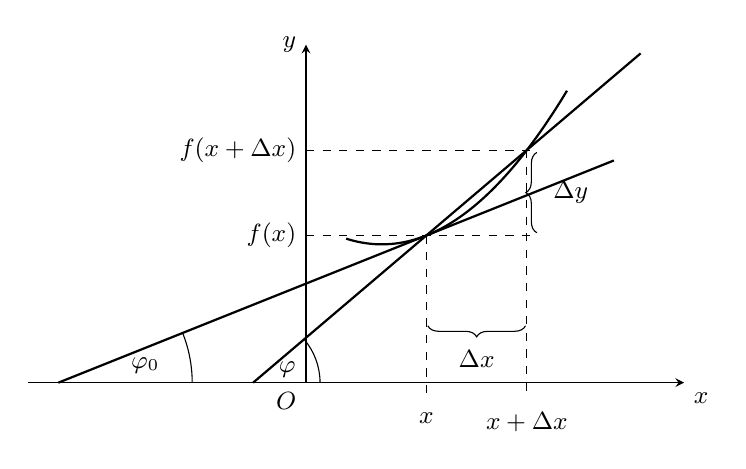
\begin{tikzpicture}[scale=0.85,>=stealth,font=\small]
  % 坐标轴
  \draw[->] (-3.15,0) -- (6.65,0) node[below right] {$x$};
  \draw[->] (1.0,0) -- (1.0,5.05) node[left] {$y$};
  \node[below left] at (1.0,0) {$O$};
  % 曲线 y=f(x)
  \draw[thick] plot[domain=1.6:4.9,samples=60,smooth]
    (\x,{0.30*(\x-2.8)*(\x-2.8)+0.40*(\x-2.8)+2.2});
  % 切线 (过 P(2.8,2.2), 斜率 0.40, 交 x 轴于 (-2.7,0))
  \draw[thick] (-2.7,0) -- (5.6,3.32);
  % 割线 PQ (斜率 0.85, 交 x 轴于 (0.21,0))
  \draw[thick] (0.21,0) -- (6.0,4.92);
  % 虚线
  \draw[dashed] (1.0,2.2) -- (4.45,2.2);
  \draw[dashed] (1.0,3.475) -- (4.45,3.475);
  \draw[dashed] (2.8,2.2) -- (2.8,-0.22);
  \draw[dashed] (4.3,3.475) -- (4.3,-0.22);
  % 纵坐标标注
  \node[left] at (1.0,2.2) {$f(x)$};
  \node[left] at (1.0,3.475) {$f(x+\Delta x)$};
  % 横坐标标注
  \node[below] at (2.8,-0.30) {$x$};
  \node[below] at (4.3,-0.30) {$x+\Delta x$};
  % Delta x 括号
  \draw[decorate,decoration={brace,amplitude=4pt,mirror}]
    (2.82,0.85) -- (4.28,0.85);
  \node at (3.55,0.36) {$\Delta x$};
  % Delta y 括号
  \draw[decorate,decoration={brace,amplitude=4pt}]
    (4.45,2.24) -- (4.45,3.44);
  \node[right] at (4.55,2.84) {$\Delta y$};
  % 角 φ0 (切线与 x 轴夹角)
  \draw (-2.7,0) ++(2.0,0) arc (0:21.8:2.0);
  \node at (-1.40,0.26) {$\varphi_0$};
  % 角 φ (割线与 x 轴夹角)
  \draw (0.21,0) ++(1.0,0) arc (0:40.4:1.0);
  \node at (0.72,0.20) {$\varphi$};
\end{tikzpicture}
\caption{}\label{fig:3.1.1}
\end{figure}

\begin{definition}[导数]\label{def:3.1.1}
设函数 $y = f(x)$ 在点 $x_0$ 处的某开邻域 $(x_0 - \delta_0, x_0 + \delta_0)$ (点 $x_0$ 附近)有定义. 如果极限
\[
\lim_{x\to x_0}\frac{f(x) - f(x_0)}{x - x_0} = \lim_{\Delta x\to0}\frac{f(x_0+\Delta x) - f(x_0)}{\Delta x} = \lim_{\Delta x\to0}\frac{\Delta y}{\Delta x}
\]
存在且有限, 则称函数 $f$ 在点 $x_0$ 处可导, 且称此极限值为 $f$ 在点 $x_0$ 处的导数(或变化率), 记为
\[
f'(x_0)\ \text{或}\ f'(x)|_{x=x_0}\ \text{或}\ \frac{\mathrm{d}f}{\mathrm{d}x}\Big|_{x=x_0}\ \text{或}\ y'(x_0)\ \text{或}\ \frac{\mathrm{d}y}{\mathrm{d}x}\Big|_{x=x_0},
\]
其中, $\Delta x = x - x_0$ 称为自变量 $x$ 的增量, 而 $\Delta y = f(x_0+\Delta x) - f(x_0)$ 称为函数(因变量)$y$ 的增量, $\frac{\Delta y}{\Delta x}$ 称为平均变化率.
\end{definition}

由定义~\ref{def:3.1.1} 知, 瞬时速度就是质点作直线运动的位移函数 $x(t)$ 对时间 $t$ 的导数; 直细棒的线密度就是其质量函数 $m(x)$ 对 $x$ 的导数, 这就是导数的物理意义. 切线的斜率就是 $y = f(x)$ 对 $x$ 的导数, 这是导数的几何意义.

用"$\varepsilon$-$\delta$"语言描述导数如下: $\forall \varepsilon > 0, \exists \delta > 0$, 当 $0 < |x - x_0| < \delta$ 时,
\[
\left|\frac{f(x) - f(x_0)}{x - x_0} - f'(x_0)\right| < \varepsilon,
\]
\[
\left|\frac{f(x_0+\Delta x) - f(x_0)}{\Delta x} - f'(x_0)\right| < \varepsilon.
\]

设 $f$ 在点 $x_0$ 的左旁 $(x_0 - \delta_0, x_0]$ 有定义, 如果
\[
\lim_{x\to x_0^-}\frac{f(x) - f(x_0)}{x - x_0} = \lim_{\Delta x\to0^-}\frac{f(x_0+\Delta x) - f(x_0)}{\Delta x}
\]
存在且有限, 则称此极限值为 $f$ 在点 $x_0$ 处的左导数, 记为 $f'_-(x_0)$. 类似可定义 $f$ 在点 $x_0$ 处的右导数 $f'_+(x_0)$.

\begin{theorem}\label{thm:3.1.1}
$f$ 在点 $x_0$ 处可导 $\iff f$ 在点 $x_0$ 处既左可导又右可导, 且 $f'_-(x_0) = f'_+(x_0)$.
\end{theorem}

\begin{proof}
$f$ 在点 $x_0$ 处可导, 即
\[
\lim_{x\to x_0}\frac{f(x) - f(x_0)}{x - x_0} = f'(x_0) \in \mathbb{R}
\]
\[
\iff f'_-(x_0) = \lim_{x\to x_0^-}\frac{f(x) - f(x_0)}{x - x_0} = \lim_{x\to x_0^+}\frac{f(x) - f(x_0)}{x - x_0} = f'_+(x_0) \in \mathbb{R},
\]
且 $f'_-(x_0) = f'(x_0) = f'_+(x_0)$.
\end{proof}

\begin{definition}\label{def:3.1.2}
如果 $y = f(x)$ 在开区间 $(a,b)$ 内的任一点 $x$ 处可导, 则称 $f$ 在 $(a,b)$ 内可导; 如果 $f$ 在有界区间 $(a,b)$ 内可导, 又在 $a$ 处右可导, 在 $b$ 处左可导, 则称 $f$ 在闭区间 $[a,b]$ 上可导.
\end{definition}

$f(x)$ 在区间 $I$ 中的导数形成一个新函数 $f'(x)$, 称为 $f(x)$ 的导函数. 如果 $f'(x)$ 为 $I$ 上的连续函数, 即 $\lim\limits_{x\to x_0}f'(x) = f'(x_0)$, $\forall x_0 \in I$, 则称 $f$ 为 $1$ 阶连续可导的函数.

注意, $f'_-(x_0)$ ($f'_+(x_0)$)为 $f$ 在点 $x_0$ 处的左(右)导数, 但是 $f'(x_0^-) = \lim\limits_{x\to x_0^-}f'(x)$ ($f'(x_0^+) = \lim\limits_{x\to x_0^+}f'(x)$)为导函数 $f'(x)$ 在点 $x_0$ 处的左(右)极限.

\begin{theorem}\label{thm:3.1.2}
设 $f$ 在点 $x_0$ 处可导, 则 $f$ 在点 $x_0$ 处连续. 反之不真.
\end{theorem}

\begin{proof}
($\Rightarrow$) 设 $f$ 在点 $x_0$ 处可导, 则
\[
\lim_{x\to x_0}f(x) = \lim_{x\to x_0}\left[\frac{f(x) - f(x_0)}{x - x_0}(x - x_0) + f(x_0)\right] = f'(x_0)\cdot0 + f(x_0) = f(x_0).
\]
这就证明了 $f$ 在点 $x_0$ 处连续.

($\Leftarrow$) 反例: $f(x) = |x|$ 在 $x_0 = 0$ 处连续, 但在 $x_0 = 0$ 处不可导.

事实上, 由
\[
f'_+(0) = \lim_{x\to0^+}\frac{f(x) - f(0)}{x - 0} = \lim_{x\to0^+}\frac{x - 0}{x - 0} = \lim_{x\to0^+}1 = 1
\]
\[
\neq -1 = \lim_{x\to0^-}(-1) = \lim_{x\to0^-}\frac{(-x) - 0}{x - 0} = \lim_{x\to0^-}\frac{f(x) - f(0)}{x - 0} = f'_-(0)
\]
及定理~\ref{thm:3.1.1} 得到: $f$ 在 $x_0 = 0$ 处不可导.
\end{proof}

\begin{theorem}[求导的四则运算法则]\label{thm:3.1.3}
设 $f$, $g$ 在点 $x$ 处可导, 则 $f \pm g$, $cf$($c$ 为常数), $fg$, $\frac{f}{g}$($g(x) \neq 0$)都在点 $x$ 处可导, 且
\begin{enumerate}[label=(\arabic*)]
  \item $(f \pm g)' = f' \pm g'$ (线性性);
  \item $(cf)' = cf'$ (线性性);
  \item $(fg)' = f'g + fg'$;
  \item $\left(\frac{f}{g}\right)' = \frac{f'g - fg'}{g^2}$.
\end{enumerate}
\end{theorem}

\begin{proof}
(1)
\[
\begin{aligned}
(f \pm g)'(x) &= \lim_{\Delta x\to0}\frac{(f \pm g)(x+\Delta x) - (f \pm g)(x)}{\Delta x}\\
&= \lim_{\Delta x\to0}\frac{[f(x+\Delta x) - f(x)] \pm [g(x+\Delta x) - g(x)]}{\Delta x}\\
&= f'(x) \pm g'(x).
\end{aligned}
\]
(2)
\[
\begin{aligned}
(cf)'(x) &= \lim_{\Delta x\to0}\frac{(cf)(x+\Delta x) - (cf)(x)}{\Delta x}\\
&= c\lim_{\Delta x\to0}\frac{f(x+\Delta x) - f(x)}{\Delta x} = cf'(x).
\end{aligned}
\]
(3) 由 $g$ 在点 $x$ 处可导及定理~\ref{thm:3.1.2} 推得 $g$ 在点 $x$ 处连续, 于是有
\[
\begin{aligned}
(fg)'(x) &= \lim_{\Delta x\to0}\frac{(fg)(x+\Delta x) - (fg)(x)}{\Delta x}\\
&= \lim_{\Delta x\to0}\frac{[f(x+\Delta x) - f(x)]g(x+\Delta x) + f(x)[g(x+\Delta x) - g(x)]}{\Delta x}\\
&= f'(x)g(x) + f(x)g'(x).
\end{aligned}
\]
(4) 同 (3) 知, $g$ 在点 $x$ 处连续, 故有
\[
\begin{aligned}
\left(\frac{f}{g}\right)'(x) &= \lim_{\Delta x\to0}\frac{\left(\frac{f}{g}\right)(x+\Delta x) - \left(\frac{f}{g}\right)(x)}{\Delta x}\\
&= \lim_{\Delta x\to0}\frac{1}{\Delta x}\left[\frac{f(x+\Delta x)}{g(x+\Delta x)} - \frac{f(x)}{g(x)}\right]\\
&= \lim_{\Delta x\to0}\frac{1}{g(x+\Delta x)g(x)}\\
&\quad\times\frac{[f(x+\Delta x) - f(x)]g(x+\Delta x) - f(x)[g(x+\Delta x) - g(x)]}{\Delta x}\\
&= \frac{f'(x)g(x) - f(x)g'(x)}{g^2(x)}.
\end{aligned}
\]
\end{proof}

\begin{theorem}[复合函数的求导链式规则, 简称链规则]\label{thm:3.1.4}
设 $y = y(u)$ 在点 $u_0$ 处可导, $u = u(x)$ 在点 $x_0$ 处可导, $u_0 = u(x_0)$, 则复合函数 $y = y(u(x)) = (y \circ u)(x)$ 在点 $x_0$ 处可导, 且
\[
\left(y(u(x))\right)'|_{x=x_0} = y'(u_0)u'(x_0),
\]
或
\[
y'_x|_{x=x_0} = y'_u|_{u=u_0}\cdot u'_x|_{x=x_0}.
\]
\end{theorem}

\begin{proof}
令
\[
F(\Delta u) = \begin{cases}
\dfrac{y(u_0+\Delta u) - y(u_0)}{\Delta u}, & \Delta u \neq 0,\\
y'(u_0), & \Delta u = 0,
\end{cases}
\]
则 $F(\Delta u)$ 在 $\Delta u = 0$ 处连续. 此外, 由 $u = u(x)$ 在点 $x_0$ 处可导知, $\Delta u \to 0\ (\Delta x \to 0)$. 于是,
\[
\begin{aligned}
(y(u(x)))'|_{x=x_0} &= \lim_{\Delta x\to0}\frac{y(u(x_0+\Delta x)) - y(u(x_0))}{\Delta x}\\
&= \lim_{\Delta x\to0}F(\Delta u)\cdot\frac{\Delta u}{\Delta x} = y'(u_0)u'(x_0).
\end{aligned}
\]
\end{proof}

\begin{theorem}[反函数的求导法则]\label{thm:3.1.5}
设 $y = f(x)$ 为 $x = g(y)$ 的反函数(即 $f = g^{-1}$, $g = f^{-1}$). 如果 $g(y)$ 在点 $y_0$ 的某开邻域内连续、严格单调且 $g'(y_0) \neq 0$, 则 $f(x)$ 在点 $x_0 = g(y_0)$ 处可导, 且
\[
f'(x_0) = \frac{1}{g'(y_0)} = \frac{1}{(f^{-1}(y))'|_{y=y_0}},\ \text{或}\ y'_x(x_0) = \frac{1}{x'_y(y_0)}.
\]
\end{theorem}

\begin{proof}
因为 $g$ 在点 $y_0$ 的某开邻域内连续且严格单调, 根据定理~\ref{thm:2.4.4} 知, $f = g^{-1}$ 在点 $x_0$ 的某开邻域内连续且严格单调, 从而
\[
\Delta y = f(x_0+\Delta x) - f(x_0) = 0 \iff \Delta x = g(y_0+\Delta y) - g(y_0) = 0,\quad \Delta y \to 0 \iff \Delta x \to 0.
\]
由 $g'(y_0) \neq 0$, 可得
\[
f'(x_0) = \lim_{\Delta x\to0}\frac{\Delta y}{\Delta x} = \lim_{\Delta x\to0}\frac{1}{\frac{\Delta x}{\Delta y}} = \frac{1}{g'(y_0)}.
\]
\end{proof}

\begin{example}\label{ex:3.1.5}
证明下列基本初等函数的导数:
\begin{enumerate}[label=(\arabic*)]
  \item $C' = 0$, 其中 $C$ 为常值函数;
  \item $(\sin x)' = \cos x$, $(\cos x)' = -\sin x$, $(\tan x)' = \sec^2 x$, $(\cot x)' = -\csc^2 x$, $(\sec x)' = \sec x\tan x$, $(\csc x)' = -\csc x\cot x$;
  \item $(\log_a x)' = \frac{1}{x\ln a}\ (a>0)$, $(\ln x)' = \frac{1}{x}$, $(\ln|x|)' = \frac{1}{x}$;
  \item $(x^\mu)' = \mu x^{\mu-1}$;
  \item $(a^x)' = a^x\ln a$, $(\mathrm{e}^x)' = \mathrm{e}^x$;
  \item $(\arcsin x)' = \frac{1}{\sqrt{1-x^2}}$, $(\arccos x)' = -\frac{1}{\sqrt{1-x^2}}$, $(\arctan x)' = \frac{1}{1+x^2}$, $(\operatorname{arccot} x)' = -\frac{1}{1+x^2}$.
\end{enumerate}
\end{example}

\begin{proof}
(1) $C' = \lim\limits_{\Delta x\to0}\frac{C - C}{\Delta x} = \lim\limits_{\Delta x\to0}0 = 0$.

(2)
\[
\begin{aligned}
(\sin x)' &= \lim_{\Delta x\to0}\frac{\sin(x+\Delta x) - \sin x}{\Delta x} = \lim_{\Delta x\to0}\frac{2\cos\frac{2x+\Delta x}{2}\sin\frac{\Delta x}{2}}{\Delta x}\\
&= \lim_{\Delta x\to0}\cos\frac{2x+\Delta x}{2}\cdot\frac{\sin\frac{\Delta x}{2}}{\frac{\Delta x}{2}} = \cos x\cdot1 = \cos x.
\end{aligned}
\]
或者
\[
\begin{aligned}
(\sin x)'|_{x=x_0} &= \lim_{x\to x_0}\frac{\sin x - \sin x_0}{x - x_0} = \lim_{x\to x_0}\cos\frac{x+x_0}{2}\cdot\frac{\sin\frac{x-x_0}{2}}{\frac{x-x_0}{2}}\\
&= \cos x_0\cdot1 = \cos x_0.
\end{aligned}
\]
所以, $(\sin x)' = \cos x$.
\[
\begin{aligned}
(\cos x)' &= \lim_{\Delta x\to0}\frac{\cos(x+\Delta x) - \cos x}{\Delta x} = -\lim_{\Delta x\to0}\frac{2\sin\frac{2x+\Delta x}{2}\sin\frac{\Delta x}{2}}{\Delta x}\\
&= -\sin x\cdot1 = -\sin x.
\end{aligned}
\]
或者
\[
(\cos x)' = \left[\sin\left(\frac{\pi}{2} - x\right)\right]' = \cos\left(\frac{\pi}{2} - x\right)\cdot(-1) = -\sin x.
\]
\[
(\tan x)' = \left(\frac{\sin x}{\cos x}\right)' = \frac{\cos x\cdot\cos x - \sin x\cdot(-\sin x)}{\cos^2 x} = \frac{1}{\cos^2 x} = \sec^2 x.
\]
\[
(\cot x)' = \left(\frac{\cos x}{\sin x}\right)' = \frac{(-\sin x)\sin x - \cos x\cdot\cos x}{\sin^2 x} = -\frac{1}{\sin^2 x} = -\csc^2 x.
\]
\[
(\sec x)' = \left(\frac{1}{\cos x}\right)' = \frac{0\cdot\cos x - 1\cdot(-\sin x)}{\cos^2 x} = \sec x\tan x.
\]
\[
(\csc x)' = \left(\frac{1}{\sin x}\right)' = \frac{0\cdot\sin x - 1\cdot\cos x}{\sin^2 x} = -\csc x\cot x.
\]
(3)
\[
\begin{aligned}
(\log_a x)' &= \lim_{\Delta x\to0}\frac{\log_a(x+\Delta x) - \log_a x}{\Delta x}\\
&= \frac{1}{x}\lim_{\Delta x\to0}\log_a\left(1+\frac{\Delta x}{x}\right)^{\frac{x}{\Delta x}} = \frac{1}{x}\log_a\mathrm{e} = \frac{1}{x\ln a}.
\end{aligned}
\]
特别地,
\[
(\ln|x|)' = \begin{cases}
(\ln x)' = \dfrac{1}{x}, & x > 0,\\
(\ln(-x))' = \dfrac{1}{-x}\cdot(-1) = \dfrac{1}{x}, & x < 0
\end{cases} = \frac{1}{x}.
\]
(4)
\[
(x^\mu)' = (\mathrm{e}^{\mu\ln x})' = \mathrm{e}^{\mu\ln x}\cdot\mu\cdot\frac{1}{x} = x^\mu\cdot\frac{\mu}{x} = \mu x^{\mu-1}.
\]
当 $\mu = n \in \mathbb{N}$ 时, 还可如下证明:
\[
\begin{aligned}
(x^n)' &= \lim_{\Delta x\to0}\frac{(x+\Delta x)^n - x^n}{\Delta x} = \lim_{\Delta x\to0}\sum_{k=1}^{n}C_n^k x^{n-k}(\Delta x)^{k-1}\\
&= C_n^1 x^{n-1} = nx^{n-1}.
\end{aligned}
\]
当 $x > 0$ 时, $(\sqrt{x})' = (x^{\frac{1}{2}})' = \frac{1}{2}x^{-\frac{1}{2}} = \frac{1}{2\sqrt{x}}$. 当 $x = 0$ 时,
\[
(\sqrt{x})'|_{x=0} = \lim_{x\to0^+}\frac{\sqrt{x} - \sqrt{0}}{x - 0} = \lim_{x\to0^+}\frac{1}{\sqrt{x}} = +\infty.
\]
所以, $\sqrt{x}$ 在 $x=0$ 处非右可导, 但它有右切线, 其斜率为 $\tan\varphi_0 = +\infty$, $\varphi_0 = \frac{\pi}{2}$, 即切线为 $y$ 轴.

(5)
\[
(a^x)' = \lim_{\Delta x\to0}\frac{a^{x+\Delta x} - a^x}{\Delta x} = a^x\cdot\lim_{\Delta x\to0}\frac{a^{\Delta x} - 1}{\Delta x} = a^x\ln a.
\]
或应用反函数求导法则的定理~\ref{thm:3.1.5} 得到
\[
(a^x)' = \frac{1}{(\log_a y)'} = \frac{1}{\frac{1}{y\ln a}} = y\ln a = a^x\ln a.
\]
(6) $y = \arcsin x$, $x = \sin y$, 由反函数求导法则的定理~\ref{thm:3.1.5} 得到
\[
(\arcsin x)' = y'_x = \frac{1}{x'_y} = \frac{1}{\cos y} = \frac{1}{\sqrt{1-\sin^2 y}} = \frac{1}{\sqrt{1-x^2}},
\]
其中 $y \in \left(-\frac{\pi}{2}, \frac{\pi}{2}\right)$, 故 $\cos y > 0$. 类似可得
\[
(\arccos x)' = -\frac{1}{\sqrt{1-x^2}},\quad (\arctan x)' = \frac{1}{1+x^2},\quad (\operatorname{arccot} x)' = -\frac{1}{1+x^2}.
\]
\end{proof}

由例~\ref{ex:3.1.5} 与定理~\ref{thm:3.1.3} 与定理~\ref{thm:3.1.4} 可以计算任何初等函数的导数.

\begin{example}\label{ex:3.1.6}
求下列函数的导数:
\begin{enumerate}[label=(\arabic*)]
  \item $f(x) = a_0 x^n + a_1 x^{n-1} + \cdots + a_{n-1}x + a_n$;
  \item $f(x) = \ln(x + \sqrt{1+x^2})$;
  \item $y = x^x$;
  \item $y = u(x)^{v(x)}$, 其中 $u(x) > 0$, 且 $u(x)$ 与 $v(x)$ 均可导.
\end{enumerate}
\end{example}

\begin{solution}
(1) $f'(x) = na_0 x^{n-1} + (n-1)a_1 x^{n-2} + \cdots + a_{n-1}$.

(2)
\[
f'(x) = (\ln(x+\sqrt{1+x^2}))' = \frac{1}{x+\sqrt{1+x^2}}\left(1+\frac{2x}{2\sqrt{1+x^2}}\right) = \frac{1}{\sqrt{1+x^2}}.
\]
(3)
\[
y' = (x^x)' = (\mathrm{e}^{x\ln x})' = \mathrm{e}^{x\ln x}\cdot\left(\ln x + x\cdot\frac{1}{x}\right) = x^x(\ln x + 1).
\]
或者, 由 $y = x^x$, $\ln y = x\ln x$, $\frac{y'}{y} = \ln x + x\cdot\frac{1}{x} = \ln x + 1$, 得 $y' = x^x(\ln x + 1)$.

(4)
\[
\begin{aligned}
y' &= (u(x)^{v(x)})' = (\mathrm{e}^{v(x)\ln u(x)})'\\
&= \mathrm{e}^{v(x)\ln u(x)}\left[v'(x)\ln u(x) + v(x)\frac{u'(x)}{u(x)}\right]\\
&= u(x)^{v(x)}v'(x)\ln u(x) + u(x)^{v(x)-1}u'(x)v(x).
\end{aligned}
\]
\end{solution}

\begin{example}[对数求导法]\label{ex:3.1.7}
求
\[
y = \frac{(x+5)^2(x-4)^{\frac{1}{3}}}{(x+2)^5(x+4)^{\frac{1}{2}}}
\]
的导数 $y'$.
\end{example}

\begin{solution}
\[
\ln|y| = 2\ln|x+5| + \frac{1}{3}\ln|x-4| - 5\ln|x+2| - \frac{1}{2}\ln|x+4|,
\]
\[
\frac{y'}{y} = \frac{2}{x+5} + \frac{1}{3(x-4)} - \frac{5}{x+2} - \frac{1}{2(x+4)},
\]
\[
y' = \frac{(x+5)^2(x-4)^{\frac{1}{3}}}{(x+2)^5(x+4)^{\frac{1}{2}}}\left[\frac{2}{x+5} + \frac{1}{3(x-4)} - \frac{5}{x+2} - \frac{1}{2(x+4)}\right].
\]
\end{solution}

\begin{example}\label{ex:3.1.8}
求 $f(x) = |x+1|^3 = \begin{cases}(x+1)^3, & x \geqslant -1,\\ -(x+1)^3, & x < -1\end{cases}$ 的导函数 $f'(x)$, 并说明其连续性.
\end{example}

\begin{solution}
因为
\[
f'_+(-1) = \lim_{x\to(-1)^+}\frac{(x+1)^3 - 0}{x - (-1)} = \lim_{x\to(-1)^+}(x+1)^2 = 0,
\]
\[
f'_-(-1) = \lim_{x\to(-1)^-}\frac{-(x+1)^3 - 0}{x - (-1)} = -\lim_{x\to(-1)^-}(x+1)^2 = 0,
\]
所以, $f'(-1) = 0$. 于是
\[
f'(x) = \begin{cases}3(x+1)^2, & x \geqslant -1,\\ -3(x+1)^2, & x < -1.\end{cases}
\]
易见, $f'(x)$ 在 $[-1,+\infty)$ 上与初等函数 $3(x+1)^2$ 一致, 所以 $f'(x)$ 在 $[-1,+\infty)$ 上连续. 又因为
\[
3(x+1)^2|_{x=-1} = 0 = -3(x+1)^2|_{x=-1},
\]
且 $f'(x)$ 在 $(-\infty,-1]$ 上与初等函数 $-3(x+1)^2$ 一致, 故 $f'(x)$ 在 $(-\infty,-1]$ 上连续. 从而 $f'(x)$ 在 $(-\infty,+\infty)$ 上连续.
\end{solution}

\begin{example}\label{ex:3.1.9}
设
\[
f(x) = \begin{cases}x^m\sin\dfrac{1}{x}, & x \neq 0,\\ 0, & x = 0.\end{cases}
\]
试问: (1) $m$ 为何值时, $f$ 在 $x=0$ 处连续; (2) $m$ 为何值时, $f$ 在 $x=0$ 处可导; (3) $m$ 为何值时, $f'$ 在 $x=0$ 处连续.
\end{example}

\begin{solution}
当 $m > 0$ 时, 由 $|f(x) - 0| = \left|x^m\sin\frac{1}{x} - 0\right| \leqslant |x|^m$ 知, $f(x)$ 在 $x=0$ 连续.

当 $m \leqslant 0$ 时, 由
\[
\lim_{n\to+\infty}f\left(\frac{1}{2n\pi}\right) = \lim_{n\to+\infty}0 = 0 \neq \lim_{n\to+\infty}\frac{1}{\left(2n\pi+\frac{\pi}{2}\right)^m} = \lim_{n\to+\infty}f\left(\frac{1}{2n\pi+\pi/2}\right)
\]
推得, $\lim\limits_{x\to0}f(x)$ 不存在, 所以 $f$ 在 $x=0$ 处不连续.

再考虑 $f'(x)$.
\[
\lim_{x\to0}\frac{f(x) - f(0)}{x - 0} = \lim_{x\to0}\frac{x^m\sin\frac{1}{x} - 0}{x - 0} = \lim_{x\to0}x^{m-1}\sin\frac{1}{x} = \begin{cases}0, & m > 1,\\ \text{不存在}, & m \leqslant 1.\end{cases}
\]
于是, 当 $m > 1$ 时,
\[
f'(x) = \begin{cases}mx^{m-1}\sin\dfrac{1}{x} - x^{m-2}\cos\dfrac{1}{x}, & x \neq 0,\\ 0, & x = 0.\end{cases}
\]
由上可知: (1) 当 $m > 0$ 时, $f$ 在 $x=0$ 处连续; (2) 当 $m > 1$ 时, $f$ 在 $x=0$ 处可导; (3) 当 $m > 2$ 时, $f'$ 在 $x=0$ 处连续.
\end{solution}

\begin{example}\label{ex:3.1.10}
设 $f$ 可导, 且 $f(x) > 0$, $F(x) = (f\circ f)^{\frac{1}{f}}(x)$, 求 $F'(x)$.
\end{example}

\begin{solution}
\textbf{解法 1}
\[
\begin{aligned}
F' &= ((f\circ f)^{\frac{1}{f}})' = (\mathrm{e}^{\frac{1}{f}\ln(f\circ f)})'\\
&= \mathrm{e}^{\frac{1}{f}\ln(f\circ f)}\left[\frac{(f'\circ f)\cdot f'}{f\circ f}\cdot f - f'\ln(f\circ f)\right]\Big/ f^2\\
&= \frac{(f\circ f)^{\frac{1}{f}}}{(f\circ f)f^2}\left[(f'\circ f)f'f - (f\circ f)f'\ln(f\circ f)\right].
\end{aligned}
\]

\textbf{解法 2}
\[
\ln F = \frac{1}{f}\ln(f\circ f),\qquad
\frac{F'}{F} = \left[\frac{(f'\circ f)f'f}{f\circ f} - f'\ln(f\circ f)\right]\Big/ f^2,
\]
\[
F' = (f\circ f)^{\frac{1}{f}}\left[(f'\circ f)f'f - f'(f\circ f)\ln(f\circ f)\right]/(f\circ f)f^2.
\]
\end{solution}

\begin{example}\label{ex:3.1.11}
\begin{enumerate}[label=(\arabic*)]
  \item 可导的周期为 $T$ 的函数 $f$, 其导函数 $f'$ 仍为周期 $T$ 的函数.
  \item 可导的奇函数 $f$, 其导函数必为偶函数.
  \item 可导的偶函数, 其导函数必为奇函数.
\end{enumerate}
\end{example}

\begin{proof}
(1) 因为 $f(x+T) = f(x)$, $\forall x \in \mathbb{R}$, 所以
\[
f'(x) = f'(x+T)(x+T)' = f'(x+T),\quad \forall x \in \mathbb{R},
\]
即 $f'$ 仍为周期 $T$ 的函数.

(2) 因 $f(-x) = -f(x)$, $\forall x \in \mathbb{R}$, 故 $-f'(x) = f'(-x)\cdot(-1)$, $f'(-x) = f'(x)$, 从而 $f'$ 为偶函数.

(3) 因 $f(-x) = f(x)$, $\forall x \in \mathbb{R}$, 故 $f'(-x)\cdot(-1) = f'(x)$, $f'(-x) = -f'(x)$, 从而 $f'$ 为奇函数.
\end{proof}

\begin{example}\label{ex:3.1.12}
设 $f_{ij}(x)$ ($i,j = 1, 2, \cdots, n$)为可导函数. 证明:
\[
\frac{\mathrm{d}}{\mathrm{d}x}
\begin{vmatrix}
f_{11}(x) & f_{12}(x) & \cdots & f_{1n}(x)\\
f_{21}(x) & f_{22}(x) & \cdots & f_{2n}(x)\\
\vdots & \vdots & \ddots & \vdots\\
f_{n1}(x) & f_{n2}(x) & \cdots & f_{nn}(x)
\end{vmatrix}
=
\sum_{k=1}^{n}
\begin{vmatrix}
f_{11}(x) & f_{12}(x) & \cdots & f_{1n}(x)\\
\vdots & \vdots & & \vdots\\
f'_{k1}(x) & f'_{k2}(x) & \cdots & f'_{kn}(x)\\
\vdots & \vdots & & \vdots\\
f_{n1}(x) & f_{n2}(x) & \cdots & f_{nn}(x)
\end{vmatrix}.
\]
\end{example}

\begin{proof}
\[
\begin{aligned}
\text{左边} &= \frac{\mathrm{d}}{\mathrm{d}x}\sum_{\pi}(-1)^{\pi}f_{1j_1}\cdots f_{nj_n} = \sum_{\pi}(-1)^{\pi}\frac{\mathrm{d}}{\mathrm{d}x}(f_{1j_1}\cdots f_{nj_n})\\
&= \sum_{\pi}(-1)^{\pi}\sum_{k=1}^{n}f_{1j_1}\cdots\left(\frac{\mathrm{d}}{\mathrm{d}x}f_{kj_k}\right)\cdots f_{nj_n}\\
&= \sum_{k=1}^{n}\sum_{\pi}(-1)^{\pi}f_{1j_1}\cdots f'_{kj_k}\cdots f_{nj_n} = \text{右边}.
\end{aligned}
\]
\end{proof}

\begin{example}\label{ex:3.1.13}
设函数 $f$ 在 $x=0$ 处可导, $n \in \mathbb{N}$, $a_n \to 0^-$, $b_n \to 0^+$ ($n \to +\infty$). 证明:
\[
\lim_{n\to+\infty}\frac{f(b_n) - f(a_n)}{b_n - a_n} = f'(0).
\]
\end{example}

\begin{proof}
\textbf{证法 1}\quad 设 $\frac{f(x) - f(0)}{x} = f'(0) + \alpha(x)$, 则
\[
\lim_{x\to0}\alpha(x) = \lim_{x\to0}\left[\frac{f(x) - f(0)}{x} - f'(0)\right] = f'(0) - f'(0) = 0,
\]
\[
f(b_n) = f(0) + f'(0)b_n + b_n\alpha(b_n),\quad f(a_n) = f(0) + f'(0)a_n + a_n\alpha(a_n).
\]
于是,
\[
\begin{aligned}
\lim_{n\to+\infty}\frac{f(b_n) - f(a_n)}{b_n - a_n}
&= \lim_{n\to+\infty}\frac{f'(0)(b_n - a_n) + b_n\alpha(b_n) - a_n\alpha(a_n)}{b_n - a_n}\\
&= \lim_{n\to+\infty}\left[f'(0) + \alpha(b_n) + \frac{a_n}{b_n - a_n}(\alpha(b_n) - \alpha(a_n))\right]\\
&= f'(0) + 0 + 0 = f'(0),
\end{aligned}
\]
其中, $a_n < 0, b_n > 0$, $\left|\frac{a_n}{b_n - a_n}\right| < 1$.

\textbf{证法 2}\quad 因为 $f$ 在 $x=0$ 处可导, 故
\[
\lim_{n\to+\infty}\frac{f(a_n) - f(0)}{a_n - 0} = f'(0),\quad \lim_{n\to+\infty}\frac{f(b_n) - f(0)}{b_n - 0} = f'(0).
\]
于是, $\forall \varepsilon > 0, \exists N \in \mathbb{N}$, 当 $n > N$ 时, 有
\[
\left|\frac{f(a_n) - f(0)}{a_n - 0} - f'(0)\right| < \varepsilon,\quad \left|\frac{f(b_n) - f(0)}{b_n - 0} - f'(0)\right| < \varepsilon.
\]
由此推得
\[
\begin{aligned}
&\left|\frac{f(b_n) - f(a_n)}{b_n - a_n} - f'(0)\right|\\
={}&\left|\frac{f(b_n) - f(0)}{b_n - 0}\frac{b_n}{b_n - a_n} - \frac{f(a_n) - f(0)}{a_n - 0}\frac{a_n}{b_n - a_n} - f'(0)\right|\\
={}&\Bigg|\left[\frac{f(b_n) - f(0)}{b_n - 0} - f'(0)\right]\frac{b_n}{b_n - a_n} - \left[\frac{f(a_n) - f(0)}{a_n - 0} - f'(0)\right]\frac{a_n}{b_n - a_n}\Bigg|\\
\leqslant{}&\left|\frac{f(b_n) - f(0)}{b_n - 0} - f'(0)\right|\frac{b_n}{b_n - a_n} + \left|\frac{f(a_n) - f(0)}{a_n - 0} - f'(0)\right|\frac{-a_n}{b_n - a_n}\\
<{}&\varepsilon\cdot\frac{b_n}{b_n - a_n} + \varepsilon\cdot\frac{-a_n}{b_n - a_n} = \varepsilon.
\end{aligned}
\]
于是, $\lim\limits_{n\to+\infty}\frac{f(b_n) - f(a_n)}{b_n - a_n} = f'(0)$.
\end{proof}

\begin{example}\label{ex:3.1.14}
求曲线 $y = x^2$ 与 $y = \frac{1}{x}$ 交点处的夹角 $\theta$(即切线之间的夹角). 再求 $y = x^2$ 在 $(1,1)$ 点处的切线与法线(如图~\ref{fig:3.1.2} 所示).
\end{example}

\begin{solution}
曲线 $y = x^2$ 与 $y = \frac{1}{x}$ 交点 $(x,y)$ 满足联立方程
\[
\begin{cases}y = x^2,\\ y = \frac{1}{x},\end{cases}
\]
求解得到 $x^2 = \frac{1}{x}$, $x^3 = 1$, $x = 1$, $y = 1$, 所以, 此交点为 $(1,1)$.
\[
\tan\theta = \tan(\varphi_2 - \varphi_1) = \frac{\tan\varphi_2 - \tan\varphi_1}{1 + \tan\varphi_1\tan\varphi_2} = \frac{\frac{1}{x^2} - 2x}{1 + \left(-\frac{1}{x^2}\right)\cdot2x}\Big|_{x=1} = 3,
\]
$\theta = \arctan 3$. 于是, $y = x^2$ 在 $(1,1)$ 处, $y'(1) = 2x|_{x=1} = 2$.

切线: $y - 1 = 2(x-1)$, $y - 2x + 1 = 0$. 法线: $y - 1 = -\frac{1}{2}(x-1)$, $x + 2y - 3 = 0$.
\end{solution}

\begin{figure}[htbp]
\centering
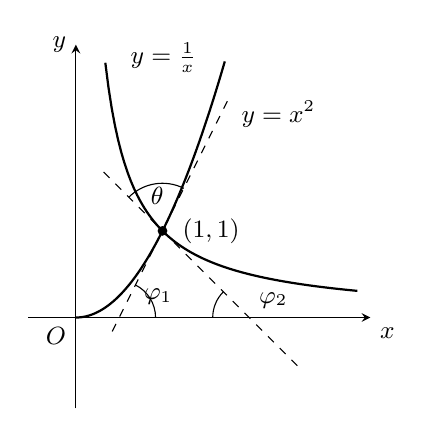
\begin{tikzpicture}[scale=1.1,>=stealth,font=\small]
  \draw[->] (-0.55,0) -- (3.40,0) node[below right] {$x$};
  \draw[->] (0,-1.05) -- (0,3.15) node[left] {$y$};
  \node[below left] at (0,0) {$O$};
  % y = x^2
  \draw[thick,domain=0:1.72,samples=60] plot (\x,{\x*\x});
  \node[right] at (1.80,2.35) {$y=x^2$};
  % y = 1/x
  \draw[thick,domain=0.34:3.25,samples=80] plot (\x,{1/\x});
  \node[right] at (0.52,3.00) {$y=\frac{1}{x}$};
  % 交点 (1,1)
  \fill (1,1) circle (1.6pt);
  \node[right] at (1.12,1.00) {$(1,1)$};
  % 切线 y=2x-1 (切于 y=x^2), 交 x 轴于 (0.5,0)
  \draw[dashed] (0.42,-0.16) -- (1.75,2.50);
  % 切线 y=-x+2 (切于 y=1/x), 交 x 轴于 (2,0)
  \draw[dashed] (0.32,1.68) -- (2.62,-0.62);
  % 夹角 theta (两切线之间)
  \draw (1,1) ++(63.4:0.55) arc (63.4:135:0.55);
  \node at (0.94,1.40) {$\theta$};
  % 角 phi_1 (y=x^2 的切线与 x 轴)
  \draw (0.5,0) ++(0.42,0) arc (0:63.4:0.42);
  \node at (0.95,0.24) {$\varphi_1$};
  % 角 phi_2 (y=1/x 的切线与 x 轴)
  \draw (2,0) ++(-0.42,0) arc (180:135:0.42);
  \node at (2.28,0.20) {$\varphi_2$};
\end{tikzpicture}
\caption{}\label{fig:3.1.2}
\end{figure}

\begin{example}\label{ex:3.1.15}
质点作直线运动, 它离原点 $O$ 的位移为 $x(t)$, 求质点运动的加速度(速度的变化率). 进而问: 在高度为 $h_0$ 处的物体作自由落体运动, 何时落到地面?
\end{example}

\begin{solution}
由例~\ref{ex:3.1.1} 知, (瞬时)速度 $v(t) = x'(t) = \lim\limits_{\Delta t\to0}\frac{x(t+\Delta t) - x(t)}{\Delta t}$, 它是质点位移 $x(t)$ 对时间 $t$ 的导数. 如果极限
\[
a(t) = v'(t) = \lim_{\Delta t\to0}\frac{v(t+\Delta t) - v(t)}{\Delta t} = \lim_{\Delta t\to0}\frac{x'(t+\Delta t) - x'(t)}{\Delta t} \xlongequal{\text{记作}} x''(t)
\]
存在且有限, 则称它为质点运动的加速度, 它是速度 $v(t)$ 对 $t$ 的导数, 也是位移 $x(t)$ 的 $2$ 阶导数.

自由落体运动, 其离地面高度 $h(t) = h_0 - \frac{1}{2}gt^2$, 速度 $v(t) = h'(t) = -gt$, 加速度 $a(t) = v'(t) = h''(t) = -g\ (\approx 980\,\text{cm/s}^2)$, 它是匀加速运动. 当 $t = \sqrt{\frac{2h_0}{g}}$ 时, 物体下落到地面.
\end{solution}

\begin{example}\label{ex:3.1.16}
汽车前灯的反光镜(或探照灯, 如图~\ref{fig:3.1.3} 所示)是由抛物线绕对称轴旋转而成的旋转抛物面. 这种反光镜就是利用抛物线的光学特性: 若光源置于抛物线的焦点上, 则光线经抛物线反射成一束平行于对称轴的光线(如图~\ref{fig:3.1.4} 所示). 试证之.
\end{example}

\begin{figure}[htbp]
\centering
\begin{minipage}[t]{0.45\textwidth}
\centering
\begin{tikzpicture}[scale=0.9,>=stealth]
  % 抛物面(旋转抛物面的轴截面)
  \draw[thick,domain=0.10:2.30,samples=80,smooth,variable=\t]
    plot ({0.18+1.67*((\t-1.20)/1.10)*((\t-1.20)/1.10)}, {\t});
  % 开口(椭圆, 后半虚线)
  \draw[thick] (1.85,2.30) arc (90:-90:0.30 and 1.10);
  \draw[dashed] (1.85,2.30) arc (90:270:0.30 and 1.10);
  % 焦点 F
  \draw[dashed] (0.62,1.20) circle (0.18);
  \fill (0.62,1.20) circle (1.4pt);
  \node[left,font=\small] at (0.42,1.20) {$F$};
  % 自焦点发出的光线经抛物面反射后平行于对称轴射出
  \foreach \y/\xb in {0.32/1.249,0.58/0.710,0.86/0.339,1.54/0.339,1.82/0.710,2.08/1.249}{
    \draw[->] (0.62,1.20) -- (\xb,\y);
    \draw[->] (\xb,\y) -- (2.75,\y);
  }
  \draw[->] (0.62,1.20) -- (2.75,1.20);
  \node[below,font=\small] at (1.45,-0.05) {探照灯};
\end{tikzpicture}
\caption{}\label{fig:3.1.3}
\end{minipage}
\hfill
\begin{minipage}[t]{0.45\textwidth}
\centering
\begin{tikzpicture}[scale=0.9,>=stealth]
  \draw[thick,domain=0.10:2.30,samples=80,smooth,variable=\t]
    plot ({0.18+1.67*((\t-1.20)/1.10)*((\t-1.20)/1.10)}, {\t});
  \draw[thick] (1.85,2.30) arc (90:-90:0.30 and 1.10);
  \draw[dashed] (1.85,2.30) arc (90:270:0.30 and 1.10);
  \draw[dashed] (0.62,1.20) circle (0.18);
  \fill (0.62,1.20) circle (1.4pt);
  \node[left,font=\small] at (0.42,1.20) {$F$};
  % 平行于对称轴的入射光线经抛物面反射后汇聚于焦点
  \foreach \y/\xb in {0.32/1.249,0.58/0.710,0.86/0.339,1.54/0.339,1.82/0.710,2.08/1.249}{
    \draw[->] (2.75,\y) -- (\xb,\y);
    \draw[->] (\xb,\y) -- (0.62,1.20);
  }
  \draw[->] (2.75,1.20) -- (0.62,1.20);
  \node[below,font=\small] at (1.45,-0.05) {太阳灶};
\end{tikzpicture}
\caption{}\label{fig:3.1.4}
\end{minipage}
\end{figure}

\begin{proof}
设抛物线的方程为 $y^2 = 2px$, 则焦点为 $F\left(\frac{p}{2}, 0\right)$. 在抛物线上任取一点 $A(x_0, y_0)$, 过 $A$ 点作切线 $L$, 记 $L$ 与线段 $AF$ 的夹角为 $\alpha$, $L$ 与 $x$ 轴的夹角为 $\beta$. 根据光学原理: 光线的入射角等于反射角. 因此, 如果能证明 $\alpha = \beta$, 则就证明了反射光线平行于 $x$ 轴(对称轴). 记 $L$ 与 $x$ 轴的交点为 $B$. 于是, $\alpha = \beta \iff AF = BF$.

将 $y^2 = 2px$ 两边关于 $x$ 求导得 $2yy' = 2p$, 所以, $y' = \frac{p}{y}$. 因此, 抛物线 $y^2 = 2px$ 在点 $A(x_0, y_0)$ 的切线 $L$ 的斜率为 $y'|_{x=x_0} = \frac{p}{y_0}$, 故 $L$ 的方程为
\[
y - y_0 = \frac{p}{y_0}(x - x_0).
\]
在上式中, 令 $y = 0$, 即得 $B$ 点坐标为 $(-x_0, 0)$. 因此,
\[
BF = \left|\frac{p}{2} + x_0\right|,
\]
\[
AF = \sqrt{\left(x_0 - \frac{p}{2}\right)^2 + y_0^2} = \sqrt{\left(x_0 - \frac{p}{2}\right)^2 + 2px_0} = \left|\frac{p}{2} + x_0\right| = BF.
\]
根据上述数学原理, 如果有一束平行于 $x$ 轴的光线经旋转抛物面反射到抛物线焦点 $F$(太阳灶就是由这原理造出来的, 以致在 $F$ 处达到高温, 如图~\ref{fig:3.1.5} 所示).
\end{proof}

\begin{figure}[htbp]
\centering
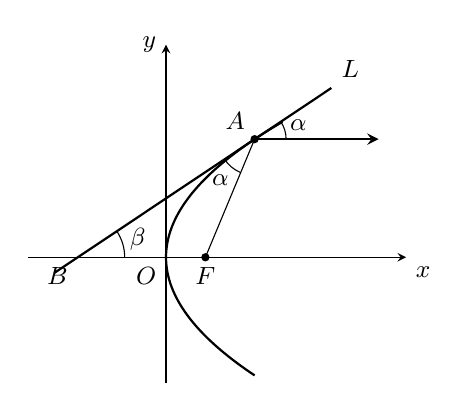
\begin{tikzpicture}[scale=1.0,>=stealth,font=\small]
  \draw[->] (-1.75,0) -- (3.05,0) node[below right] {$x$};
  \draw[->] (0,-1.60) -- (0,2.70) node[left] {$y$};
  \node[below left] at (0,0) {$O$};
  % 抛物线 y^2 = 2x  =>  x = y^2/2
  \draw[thick,domain=-1.50:1.72,samples=80,smooth,variable=\t] plot ({0.5*\t*\t},{\t});
  \coordinate (A) at (1.125,1.5);
  \coordinate (B) at (-1.125,0);
  \coordinate (F) at (0.5,0);
  % 切线 L (过 A, B)
  \draw[thick] (-1.42,-0.20) -- (2.10,2.15) node[above right] {$L$};
  % 反射光线 (平行于 x 轴)
  \draw[->,thick] (A) -- (2.70,1.5);
  % 焦半径 AF
  \draw (A) -- (F);
  \fill (A) circle (1.5pt);
  \node[above left] at (A) {$A$};
  \fill (F) circle (1.5pt);
  \node[below] at (F) {$F$};
  \node[below left] at (B) {$B$};
  % 角 beta (B 处: L 与 x 轴)
  \draw (B) ++(0.60,0) arc (0:33.7:0.60);
  \node at (-0.36,0.23) {$\beta$};
  % 角 alpha (A 处: L 与反射光线)
  \draw (A) ++(0.40,0) arc (0:33.7:0.40);
  \node at (1.68,1.68) {$\alpha$};
  % 角 alpha (A 处: L 与 AF)
  \draw (A) ++(213.7:0.46) arc (213.7:247.4:0.46);
  \node at (0.69,0.98) {$\alpha$};
\end{tikzpicture}
\caption{}\label{fig:3.1.5}
\end{figure}

\begin{exblock}{练习题 3.1}
  \item 设函数 $f$ 在点 $x_0$ 处可导, 则 $\lim\limits_{\Delta x\to0}\frac{f(x_0+\Delta x) - f(x_0-\Delta x)}{\Delta x} = 2f'(x_0)$. 举例说明: 即使上式左边的极限存在且有限, $f$ 在点 $x_0$ 处也未必可导.

  \item 在抛物线 $y = x^2$ 上哪些点的切线满足下面条件:
  \begin{enumerate}[label=(\arabic*)]
    \item 平行于直线 $y = 4x - 5$;
    \item 垂直于直线 $2x - 6y + 5 = 0$;
    \item 与直线 $3x - y + 1 = 0$ 交成 $45^\circ$ 的角.
  \end{enumerate}

  \item 证明: 抛物线 $y = x^2$ 上的两点 $(x_1, x_1^2)$ 与 $(x_2, x_2^2)$ 处的切线互相垂直的充分必要条件是 $x_1$ 与 $x_2$ 适合关系 $4x_1x_2 + 1 = 0$.

  \item 设 $f(x) = x(x-1)^2(x-2)^3$. 求 $f'(0)$, $f'(1)$, $f'(2)$.

  \item 设 $f(x_0) = 0$, $f'(x_0) = 4$. 求极限 $\lim\limits_{\Delta x\to0}\frac{f(x_0+\Delta x)}{\Delta x}$.

  \item 确定曲线 $y = \ln x$ 上哪些点的切线平行于下列直线: (1) $y = x - 1$; (2) $y = 2x - 3$.

  \item 求下列曲线在指定点 $P$ 的切线方程与法线方程:
  \begin{enumerate}[label=(\arabic*)]
    \item $y = \frac{x^2}{4}$, $P = (2,1)$;
    \item $y = \cos x$, $P = (0,1)$.
  \end{enumerate}

  \item 求下列函数的导函数:
  \begin{enumerate}[label=(\arabic*)]
    \item $f(x) = |x|^3$;
    \item $f(x) = \begin{cases}x+1, & x \geqslant 0,\\ 1, & x < 0.\end{cases}$
  \end{enumerate}

  \item 设 $f(x) = \begin{cases}x^2, & x \geqslant 3,\\ ax+b, & x < 3.\end{cases}$ 试确定 $a$, $b$ 的值, 使 $f$ 在 $x=3$ 处可导.

  \item 设 $g(0) = g'(0) = 0$, $f(x) = \begin{cases}g(x)\sin\frac{1}{x}, & x \neq 0,\\ 0, & x = 0.\end{cases}$ 求 $f'(0)$.

  \item 设函数 $f$ 在点 $x_0$ 处存在左右导数. 证明: $f$ 在点 $x_0$ 处连续.

  \item 设函数 $f$ 在 $[a,b]$ 上连续, 且 $f(a) = f(b) = K$, $f'_+(a)\cdot f'_-(b) > 0$. 证明: 在 $(a,b)$ 内至少有一点 $\xi$, 使 $f(\xi) = K$.

  \item 设 $f$ 在 $\mathbb{R}$ 上可导, 并且 $\lim\limits_{x\to\infty}f(x) = a \in \mathbb{R}$. 证明: 必 $\exists \xi \in \mathbb{R}$, s.t. $f'(\xi) = 0$.

  \item 设函数 $f$ 在 $x = a$ 处可导, 且 $f(a) \neq 0$. 求数列极限
  \[
  \lim_{n\to+\infty}\left(\frac{f\left(a+\frac{1}{n}\right)}{f(a)}\right)^n.
\]

  \item 设函数 $\varphi$ 在点 $a$ 处连续, 又在 $a$ 的近旁有 $f(x) = (x-a)\varphi(x)$ 和 $g(x) = |x-a|\varphi(x)$. 证明: $f$ 在点 $a$ 处可导, 并求 $f'(a)$. 问在什么条件下 $g$ 在点 $a$ 处可导.

  \item 求下列函数在指定点的导数:
  \begin{enumerate}[label=(\arabic*)]
    \item $f(x) = 3x^4 + 2x^3 + 5$, 求 $f'(0)$, $f'(1)$;
    \item $f(x) = \frac{x}{\cos x}$, 求 $f'(0)$, $f'(\pi)$;
    \item $f(x) = \sqrt{1 + \sqrt{x}}$, 求 $f'(0)$, $f'(1)$, $f'(4)$.
  \end{enumerate}

  \item 求下列函数的导数:
  \begin{enumerate}[label=(\arabic*)]
    \item $y = x^3 - 2x - 6$;
    \item $y = \sqrt{x} - \frac{1}{x}$;
    \item $y = \frac{1-x^2}{1+x+x^2}$;
    \item $y = \frac{x}{m} + \frac{m}{x} + 2\sqrt{x} + \frac{2}{\sqrt{x}}$;
    \item $y = x^3\log_3 x$;
    \item $y = \mathrm{e}^x\cos x$;
    \item $y = (x^2+1)(3x-1)(1-x^3)$;
    \item $y = \frac{\tan x}{x}$;
    \item $y = \frac{1+\ln x}{1-\ln x}$;
    \item $y = (\sqrt{x}+1)\arctan x$;
    \item $y = \frac{1+x^2}{\sin x + \cos x}$;
    \item $y = \mathrm{e}^{ax}\cos bx$;
    \item $y = \frac{\cos x - \sin x}{\cos x + \sin x}$;
    \item $y = x\sin x\ln x$;
    \item $y = \sqrt{x + \sqrt{x + \sqrt{x}}}$;
    \item $y = \ln(\cos x + \sin x)$;
    \item $y = (x^2-1)^3$;
    \item $y = \left(\frac{1+x^2}{1-x}\right)^3$;
    \item $y = \ln(\ln x)$;
    \item $y = \ln\frac{\sqrt{1+x} - \sqrt{1-x}}{\sqrt{1+x} + \sqrt{1-x}}$;
    \item $y = (\arctan x^3)^2$;
    \item $y = \arcsin(\sin^2 x)$;
    \item $y = \sin(\sin(\sin x))$;
    \item $y = \sin\left(\frac{x}{\sin\left(\frac{x}{\sin x}\right)}\right)$;
    \item $y = (x-a_1)^{a_1}(x-a_2)^{a_2}\cdots(x-a_n)^{a_n}$;
    \item $y = \sqrt[3]{\frac{(x+1)^2(x+2)^3}{(x+3)^4(x+4)^5}}$.
  \end{enumerate}

  \item 求下列函数的导数:
  \begin{enumerate}[label=(\arabic*)]
    \item $y = \frac{ax+b}{cx+d}$, 其中 $a, b, c, d$ 为常数;
    \item $y = \ln(x + \sqrt{x^2+a^2})$;
    \item $y = x^{x^x}$.
  \end{enumerate}

  \item 证明:
  \begin{enumerate}[label=(\arabic*)]
    \item $(\sinh x)' = \cosh x$;
    \item $(\cosh x)' = \sinh x$;
    \item $(\tanh x)' = \frac{1}{\cosh^2 x}$;
    \item $(\coth x)' = \frac{1}{\sinh^2 x}$.
  \end{enumerate}

  \item 以 $\operatorname{arsinh} x$, $\operatorname{arcosh} x$, $\operatorname{artanh} x$, $\operatorname{arcoth} x$ 分别表示各双曲函数的反函数. 试求下列函数的导数:
  \begin{enumerate}[label=(\arabic*)]
    \item $y = \operatorname{arsinh} x$;
    \item $y = \operatorname{arcosh} x$;
    \item $y = \operatorname{artanh} x$;
    \item $y = \operatorname{arcoth} x$.
  \end{enumerate}

  \item 设 $g$ 可导, $a$ 为实数. 对下列各函数计算 $f'(x)$, $f'(x+1)$, $f'(x-1)$:
  \begin{enumerate}[label=(\arabic*)]
    \item $f(x) = x^3$;
    \item $f(x) = g(x + g(x))$;
    \item $f(x) = g(x)g(a)$;
    \item $f(x) = g(x)g(x)$.
  \end{enumerate}

  \item 设 $f$ 为可导函数. 证明: 若 $x=1$ 时, 有 $\frac{\mathrm{d}}{\mathrm{d}x}f(x^2) = \frac{\mathrm{d}}{\mathrm{d}x}f^2(x)$, 且必有 $f'(1) = 0$ 或 $f(1) = 1$.

  \item 利用 $1 + x + \cdots + x^n$ 的和, 求出下列各式的和:
  \begin{enumerate}[label=(\arabic*)]
    \item $1 + 2x + 3x^2 + \cdots + nx^{n-1}$;
    \item $\sum\limits_{k=1}^{n}\frac{k}{2^{k-1}}$;
    \item $1^2 + 2^2 x + 3^2 x^2 + \cdots + n^2 x^{n-1}$.
  \end{enumerate}

  \item 设 $f$ 为可导函数, 求下列各函数的一阶导数:
  \begin{enumerate}[label=(\arabic*)]
    \item $y = f(\mathrm{e}^x)\mathrm{e}^{f(x)}$;
    \item $y = f(f(f(x)))$.
  \end{enumerate}

  \item 设 $\varphi$, $\psi$ 为可导函数, 求 $y'$:
  \begin{enumerate}[label=(\arabic*)]
    \item $y = \sqrt{\varphi^2(x) + \psi^2(x)}$;
    \item $y = \arctan\frac{\varphi(x)}{\psi(x)}$;
    \item $y = \log_{\varphi(x)}\psi(x)$ ($\varphi(x) > 0$, $\varphi(x) \neq 1$, $\psi(x) > 0$).
  \end{enumerate}

  \item 在曲线 $y = x^3$ 上取一点 $P$, 过 $P$ 的切线与该曲线交于 $Q$. 证明: 曲线在 $Q$ 点处的切线斜率正好是在 $P$ 点处切线斜率的 $4$ 倍.

  \item 设有一吊桥, 其铁链成抛物线型, 两端系于相距 $100$ m 高度相同的支柱上, 铁链的最低点在悬点下 $10$ m 处, 求铁链与支柱所成的角.

  \item 证明: 双曲线 $xy = a > 0$ 在各点处的切线与两坐标轴所围成的三角形的面积为常数.

  \item 有一底半径为 $R$ cm, 高为 $h$ cm 的正圆锥容器, 顶点有一小孔, 以便向容器内注水. 今以 $A\ \text{cm}^3/\text{s}$ 的速度向容器内注水, 试求容器内水位等于锥高一半时, 水面上升的速度.

  \item 水自高为 $18$ cm、底半径为 $6$ cm 的圆锥形漏斗流入直径为 $10$ cm 的圆柱形桶内. 已知漏斗水深 $12$ cm 时水面下降速度为 $1$ cm/s, 求此时桶中水面上升的速度.
\end{exblock}

\begin{exblock}{思考题 3.1}
  \item 证明: Riemann 函数 $R(x)$ 处处不可导.

  \item 构造一个可导函数 $f$, 使 $f$ 在有理点处取有理数值, 它的导函数在有理点处取无理数值.

  \item
  \begin{enumerate}[label=(\arabic*)]
    \item 构造一个连续函数, 它仅在已知点 $a_1, \cdots, a_n$ 处不可导;
    \item 构造一个函数, 它仅在点 $a_1, \cdots, a_n$ 处可导.
  \end{enumerate}

  \item 设 $f$ 为三次多项式, 且 $f(a) = f(b) = 0$. 证明: 函数 $f$ 在 $[a,b]$ 上不变号的必要充分条件是 $f'(a)f'(b) \leqslant 0$.

  \item 证明组合恒等式:
  \begin{enumerate}[label=(\arabic*)]
    \item $\sum\limits_{k=1}^{n}kC_n^k = n2^{n-1}$, $n \in \mathbb{N}$;
    \item $\sum\limits_{k=1}^{n}k^2C_n^k = n(n+1)2^{n-2}$, $n \in \mathbb{N}$.
  \end{enumerate}
  (提示: 分别对 $(1+x)^n = \sum\limits_{k=0}^{n}C_n^k x^k$ 与 $nx(1+x)^{n-1} = \sum\limits_{k=1}^{n}kC_n^k x^{k-1}$ 两边关于 $x$ 求导.)

  \item 设 $f(0) = 0$, $f'(0)$ 存在且有限, 令 $x_n = f\left(\frac{1}{n^2}\right) + f\left(\frac{2}{n^2}\right) + \cdots + f\left(\frac{n}{n^2}\right)$. 证明: $\lim\limits_{n\to+\infty}x_n = \frac{f'(0)}{2}$. 并利用以上结果计算:
  \begin{enumerate}[label=(\arabic*)]
    \item $\lim\limits_{n\to+\infty}\sum\limits_{k=1}^{n}\sin\frac{k}{n^2}$;
    \item $\lim\limits_{n\to+\infty}\prod\limits_{k=1}^{n}\left(1 + \frac{k}{n^2}\right)$, 其中 $\prod\limits_{k=1}^{n}$ 表示 $n$ 个数连乘.
  \end{enumerate}

  \item 设函数 $f$ 在 $x=0$ 处连续, 如果 $\lim\limits_{x\to0}\frac{f(2x) - f(x)}{x} = m$, 证明: $f'(0) = m$.

  \item 在区间 $[-1,1]$ 上讨论二次函数 $f(x) = ax^2 + bx + c$, 如果 $|f(x)| \leqslant 1$, $\forall x \in [-1,1]$, 证明: $|f'(x)| \leqslant 4$, $\forall x \in [-1,1]$.

  \item (1) 设 $f_n$, $f$ 为 $\mathbb{R}$ 上的一元函数, $f_n$ 在 $\mathbb{R}$ 上连续, $n = 1, 2, \cdots$, 且 $\lim\limits_{n\to+\infty}f_n(x) = f(x)$, $x \in \mathbb{R}$. 证明: 存在 $(\alpha,\beta) \subset \mathbb{R}$, 使得 $f$ 在 $(\alpha,\beta)$ 上是有界的.
  (2) 设 $g$ 在 $\mathbb{R}$ 上可导. 证明: 存在 $(\alpha,\beta) \subset \mathbb{R}$, 使得 $g'$ 在 $(\alpha,\beta)$ 上有界.
  (3) 使得导函数 $g'$ 在任何开区间 $(\alpha,\beta) \subset \mathbb{R}$ 上都无界的函数 $g$ 是不存在的.

  \item 在 $[0,1]$ 上适合条件 $|P| \leqslant 1$ 的二次多项式 $P$ 的全体记为 $V$, 求 $\sup\{|P'(0)|\}$.
\end{exblock}

% ====================================================================
%  徐森林、薛春华《数学分析》（第一册）
%  \S3.2  高阶导数、参变量函数的导数、导数的 Leibniz 公式
%  源：原书印刷页 171-185（PDF 物理页 177-191）
%  底本：PaddleOCR-VL-1.6 + 高清影印比对校订
%  规范：全西文半角标点；单一落盘出口 _texout.py
% ====================================================================
\section{高阶导数、参变量函数的导数、导数的 Leibniz 公式}\label{sec:3.2}

例~\ref{ex:3.1.15} 指出, 加速度就是位移对时间 $t$ 的 2 阶导数. 自然会想到要进一步研究高阶导数.

\begin{definition}\label{def:3.2.1}
如果 $f$ 的导函数 $f'$ 在点 $x_0$ 处可导, 则称 $f'$ 在点 $x_0$ 处的导数为 $f$ 在点 $x_0$ 的 2 阶导数, 记作
\[
f''(x_0) = \lim_{x\to x_0}\frac{f'(x) - f'(x_0)}{x - x_0} = \lim_{\Delta x\to0}\frac{f'(x_0+\Delta x) - f'(x_0)}{\Delta x}.
\]
同时称 $f$ 在点 $x_0$ 处 2 阶可导. 2 阶导数也可记为 $\left.\frac{\mathrm{d}^{2}f}{\mathrm{d}x^{2}}\right|_{x=x_0}$, $\left.\frac{\mathrm{d}^{2}y}{\mathrm{d}x^{2}}\right|_{x=x_0}$.

类似可定义 3 阶, 4 阶, $\cdots$, $n$ 阶导数:
\[
\begin{aligned}
f^{(n)}(x_0) &= \lim_{x\to x_0}\frac{f^{(n-1)}(x) - f^{(n-1)}(x_0)}{x - x_0}\\
&= \lim_{\Delta x\to0}\frac{f^{(n-1)}(x_0+\Delta x) - f^{(n-1)}(x_0)}{\Delta x},
\end{aligned}
\]
$f'' = (f')'$, $f^{(4)} = (f''')'$, $\cdots$, $f^{(n)} = (f^{(n-1)})'$. $n$ 阶导数也可记为 $\left.\frac{\mathrm{d}^{n}f}{\mathrm{d}x^{n}}\right|_{x=x_0}$, $\left.\frac{\mathrm{d}^{n}y}{\mathrm{d}x^{n}}\right|_{x=x_0}$.

$f$ 在开区间 $(a,b)$ 的每一点处 $n$ 阶可导, 则称 $f$ 在 $(a,b)$ 上 $n$ 阶可导.
\end{definition}

由 $n$ 阶导数定义, 显然有
\[
(f \pm g)^{(n)} = f^{(n)} \pm g^{(n)},\quad (\lambda f)^{(n)} = \lambda f^{(n)},\ \lambda \in \mathbb{R}.
\]

\begin{theorem}[Leibniz]\label{thm:3.2.1}
设 $f$ 与 $g$ 在区间 $I$ 上都 $n$ 阶可导, 则
\[
(fg)^{(n)} = \sum_{k=0}^{n}\mathrm{C}_{n}^{k}f^{(n-k)}g^{(k)},
\]
其中, $\mathrm{C}_{n}^{k} = \frac{n!}{k!(n-k)!}$ 为组合数, $g^{(0)} = g$, $f^{(0)} = f$.
\end{theorem}

\begin{proof}
用归纳法. 当 $n = 1$ 时,
\[
(fg)' = f'g + fg' = \sum_{k=0}^{1}\mathrm{C}_{1}^{k}f^{(1-k)}g^{(k)}.
\]
假设 $n = l$ 时, 有
\[
(fg)^{(l)} = \sum_{k=0}^{l}\mathrm{C}_{l}^{k}f^{(l-k)}g^{(k)}.
\]
那么, 当 $n = l+1$ 时, 有
\[
\begin{aligned}
(fg)^{(l+1)} &= ((fg)^{(l)})' = \left(\sum_{k=0}^{l}\mathrm{C}_{l}^{k}f^{(l-k)}g^{(k)}\right)'\\
&= \sum_{k=0}^{l}\mathrm{C}_{l}^{k}\left[(f^{(l-k)})'g^{(k)} + f^{(l-k)}(g^{(k)})'\right]\\
&= \sum_{k=0}^{l}\mathrm{C}_{l}^{k}\left[f^{(l+1-k)}g^{(k)} + f^{(l-k)}g^{(k+1)}\right]\\
&= \mathrm{C}_{l}^{0}f^{(l+1)}g + \sum_{k=1}^{l}\mathrm{C}_{l}^{k}f^{(l+1-k)}g^{(k)} + \sum_{k=0}^{l-1}\mathrm{C}_{l}^{k}f^{(l-k)}g^{(k+1)} + \mathrm{C}_{l}^{l}fg^{(l+1)}\\
&= \mathrm{C}_{l+1}^{0}f^{(l+1)}g + \sum_{k=1}^{l}(\mathrm{C}_{l}^{k} + \mathrm{C}_{l}^{k-1})f^{(l+1-k)}g^{(k)} + \mathrm{C}_{l+1}^{l+1}fg^{(l+1)}\\
&= \sum_{k=0}^{l+1}\mathrm{C}_{l+1}^{k}f^{(l+1-k)}g^{(k)}.
\end{aligned}
\]
\end{proof}

\begin{example}\label{ex:3.2.1}
求 $y = x^{n}$ 的各阶导函数, $n \in \mathbb{N}$.
\end{example}

\begin{solution}
\[
\begin{aligned}
y' &= nx^{n-1},\\
y'' &= n(n-1)x^{n-2},\\
&\cdots\\
y^{(n-1)} &= n(n-1)\cdots2x,\\
y^{(n)} &= n!,\\
y^{(n+1)} &= y^{(n+2)} = \cdots = 0.
\end{aligned}
\]
\end{solution}

\begin{example}\label{ex:3.2.2}
求下列函数的各阶导函数:
(1) $y = a^{x}$ ($a > 0$), 特别地, $y = \mathrm{e}^{x}$; (2) $y = \mathrm{e}^{ax}$;
(3) $y = \sin x$; (4) $y = \cos x$; (5) $y = \frac{1}{x-a}$; (6) $y = \frac{1}{x^{2}-3x+2}$.
\end{example}

\begin{solution}
(1) $y' = a^{x}\ln a$, $\cdots$, $y^{(n)} = a^{x}(\ln a)^{n}$. 特别地, $\left(\mathrm{e}^{x}\right)^{(n)} = \mathrm{e}^{x}$.

(2) $y' = a\mathrm{e}^{ax}$, $\cdots$, $y^{(n)} = a^{n}\mathrm{e}^{ax}$.

(3) $y' = \cos x = \sin\left(x + \frac{\pi}{2}\right)$. 设 $y^{(k)} = \sin\left(x + \frac{k\pi}{2}\right)$, 则有
\[
y^{(k+1)} = (y^{(k)})' = \cos\left(x + \frac{k\pi}{2}\right)\cdot1 = \sin\left[x + \frac{(k+1)\pi}{2}\right].
\]
于是, $\forall n \in \mathbb{N}$, 有
\[
y^{(n)} = \sin\left(x + \frac{n\pi}{2}\right).
\]

(4) 类似 (3), 可证 $(\cos x)^{(n)} = \cos\left(x + \frac{n\pi}{2}\right)$, $n \in \mathbb{N}$. 或者
\[
\begin{aligned}
(\cos x)^{(n)} &= \left(\sin\left(x + \frac{\pi}{2}\right)\right)^{(n)} = \sin\left(x + \frac{\pi}{2} + \frac{n\pi}{2}\right)\\
&= \cos\left(x + \frac{n\pi}{2}\right).
\end{aligned}
\]

(5) $y = \frac{1}{x-a} = (x-a)^{-1}$,
\[
y' = -(x-a)^{-2},\quad y'' = 2(x-a)^{-3},\quad \cdots,
\]
\[
y^{(n)} = (-1)^{n}\cdot n!(x-a)^{-(n+1)} = \frac{(-1)^{n}\cdot n!}{(x-a)^{(n+1)}}.
\]

(6)
\[
\begin{aligned}
y &= \frac{1}{x^{2}-3x+2} = \frac{1}{x-2} - \frac{1}{x-1},\\
y^{(n)} &= \left(\frac{1}{x-2}\right)^{(n)} - \left(\frac{1}{x-1}\right)^{(n)} = \frac{(-1)^{n}n!}{(x-2)^{n+1}} - \frac{(-1)^{n}n!}{(x-1)^{n+1}}\\
&= (-1)^{n}n!\left[\frac{1}{(x-2)^{n+1}} - \frac{1}{(x-1)^{n+1}}\right].
\end{aligned}
\]
\end{solution}

\begin{example}\label{ex:3.2.3}
设 $f(x) = a_{n}(x-x_0)^{n} + a_{n-1}(x-x_0)^{n-1} + \cdots + a_{1}(x-x_0) + a_{0}$ 为 $n$ 次多项式, 其中 $a_{n} \neq 0$,
\[
a_{k} = \frac{f^{(k)}(x_0)}{k!},\quad k = 0, 1, \cdots, n,
\]
因此,
\[
f(x) = \sum_{k=0}^{n}a_{k}(x-x_0)^{k} = \sum_{k=0}^{n}\frac{f^{(k)}(x_0)}{k!}(x-x_0)^{k}.
\]
\end{example}

\begin{proof}
因为
\[
\begin{aligned}
f(x) &= \sum_{k=0}^{n}a_{k}(x-x_0)^{k},\\
f'(x) &= \sum_{k=1}^{n}ka_{k}(x-x_0)^{k-1},\\
&\cdots\\
f^{(l)}(x) &= \sum_{k=l}^{n}k(k-1)\cdots(k-l+1)a_{k}(x-x_0)^{k-l},\\
&\cdots\\
f^{(n)}(x) &= n!a_{n},
\end{aligned}
\]
所以, $f(x_0) = a_0$, $f'(x_0) = a_1$, $\cdots$, $f^{(l)}(x_0) = l!a_l$, $\cdots$, $f^{(n)}(x_0) = n!a_n$, 即
\[
a_{l} = \frac{f^{(l)}(x_0)}{l!},\quad l = 0, 1, \cdots, n.
\]
\end{proof}

\begin{example}\label{ex:3.2.4}
设 $y = \mathrm{e}^{x}\cos x$, 求 $y^{(n)}$, $y^{(5)}$.
\end{example}

\begin{solution}
因为 $(\mathrm{e}^{x})^{(k)} = \mathrm{e}^{x}$, $(\cos x)^{(k)} = \cos\left(x + \frac{k\pi}{2}\right)$, 故由 Leibniz 求导公式知
\[
\begin{aligned}
y^{(n)} &= \left(\mathrm{e}^{x}\cos x\right)^{(n)} = \sum_{k=0}^{n}\mathrm{C}_{n}^{k}\left(\mathrm{e}^{x}\right)^{(n-k)}\left(\cos x\right)^{(k)}\\
&= \sum_{k=0}^{n}\mathrm{C}_{n}^{k}\mathrm{e}^{x}\cos\left(x + \frac{k\pi}{2}\right),
\end{aligned}
\]
当 $n = 5$ 时,
\[
\begin{aligned}
y^{(5)} &= \sum_{k=0}^{5}\mathrm{C}_{5}^{k}\mathrm{e}^{x}\cos\left(x + \frac{k\pi}{2}\right)\\
&= \mathrm{e}^{x}\left[\cos x + 5\cos\left(x + \frac{\pi}{2}\right) + 10\cos\left(x + \frac{2\pi}{2}\right) + 10\cos\left(x + \frac{3\pi}{2}\right)\right.\\
&\quad \left. + 5\cos\left(x + \frac{4\pi}{2}\right) + \cos\left(x + \frac{5\pi}{2}\right)\right]\\
&= \mathrm{e}^{x}(\cos x - 5\sin x - 10\cos x + 10\sin x + 5\cos x - \sin x)\\
&= 4\mathrm{e}^{x}(\sin x - \cos x).
\end{aligned}
\]
\end{solution}

\begin{example}\label{ex:3.2.5}
设 $y = x^{2}\cos x$, 求 $y^{(50)}$.
\end{example}

\begin{solution}
由 Leibniz 求导公式知,
\[
\begin{aligned}
y^{(50)} &= \sum_{k=0}^{50}\mathrm{C}_{50}^{k}\left(\cos x\right)^{(50-k)}\left(x^{2}\right)^{(k)}\\
&= x^{2}\left(\cos x\right)^{(50)} + \mathrm{C}_{50}^{1}\cdot2x\left(\cos x\right)^{(49)} + \mathrm{C}_{50}^{2}\cdot2\left(\cos x\right)^{(48)}\\
&= x^{2}\cos\left(x + \frac{50\pi}{2}\right) + 100x\cos\left(x + \frac{49\pi}{2}\right) + 2450\cos\left(x + \frac{48\pi}{2}\right)\\
&= -x^{2}\cos x - 100x\sin x + 2450\cos x\\
&= (2450 - x^{2})\cos x - 100x\sin x.
\end{aligned}
\]
\end{solution}

\begin{example}\label{ex:3.2.6}
设
\[
f(x) = \begin{cases}x^{4}\sin\frac{1}{x}, & x \neq 0,\\ 0, & x = 0,\end{cases}
\]
求 $f''(x)$.
\end{example}

\begin{solution}
由
\[
f'(0) = \lim_{x\to0}\frac{f(x) - f(0)}{x - 0} = \lim_{x\to0}\frac{x^{4}\sin\frac{1}{x} - 0}{x - 0} = \lim_{x\to0}x^{3}\sin\frac{1}{x} = 0,
\]
得到
\[
f'(x) = \begin{cases}4x^{3}\sin\frac{1}{x} - x^{2}\cos\frac{1}{x}, & x \neq 0,\\ 0, & x = 0.\end{cases}
\]
按照 2 阶导数定义, 有
\[
\begin{aligned}
f''(0) &= \lim_{x\to0}\frac{f'(x) - f'(0)}{x - 0} = \lim_{x\to0}\frac{4x^{3}\sin\frac{1}{x} - x^{2}\cos\frac{1}{x} - 0}{x - 0}\\
&= \lim_{x\to0}\left(4x^{2}\sin\frac{1}{x} - x\cos\frac{1}{x}\right) = 0,
\end{aligned}
\]
从而
\[
\begin{aligned}
f''(x) &= \begin{cases}12x^{2}\sin\frac{1}{x} - 4x\cos\frac{1}{x} - 2x\cos\frac{1}{x} - \sin\frac{1}{x}, & x \neq 0,\\ 0, & x = 0\end{cases}\\
&= \begin{cases}(12x^{2} - 1)\sin\frac{1}{x} - 6x\cos\frac{1}{x}, & x \neq 0,\\ 0, & x = 0.\end{cases}
\end{aligned}
\]
进一步, 由于极限
\[
\lim_{x\to0}\frac{(12x^{2} - 1)\sin\frac{1}{x} - 6x\cos\frac{1}{x} - 0}{x - 0} = \lim_{x\to0}\left[12x\sin\frac{1}{x} - \frac{\sin\frac{1}{x} + 6x\cos\frac{1}{x}}{x}\right]
\]
不存在, 故 $\forall n \in \mathbb{N}$, $f^{(n)}(x)$ 对 $x \neq 0$ 都是存在的, 但是 $f'''(0)$ 已不存在.
\end{solution}

\begin{definition}\label{def:3.2.2}
设函数 $f$ 在 $U \subsetneq \mathbb{R}$ 上连续, 则称 $f$ 在 $U$ 上是 $C^{0}$ 的, 记 $U$ 上 $C^{0}$ 函数的全体为 $C^{0}(U, \mathbb{R})$; 设 $r \in \mathbb{N}$, 如果 $f$ 在开集 $U \subsetneq \mathbb{R}$ 上 $r$ 阶连续可导, 则称 $f$ 在 $U$ 上是 $C^{r}$ 的, 记 $U$ 上 $C^{r}$ 函数的全体为 $C^{r}(U, \mathbb{R})$; 如果 $f$ 在开集 $U \subsetneq \mathbb{R}$ 上各阶连续可导, 则称 $f$ 在 $U$ 上是 $C^{\infty}$ 的, 记 $U$ 上 $C^{\infty}$ 函数的全体为 $C^{\infty}(U, \mathbb{R})$; 如果 $f$ 在开集 $U \subsetneq \mathbb{R}$ 上, 每一点 $x_0 \in U$ 的邻近可展开为收敛的幂级数
\[
f(x) = \sum_{n=0}^{\infty}a_{n}(x-x_0)^{n},\quad x \in (x_0 - \delta_{x_0}, x_0 + \delta_{x_0}) \subset U,
\]
则称 $f$ 在 $U$ 上是 $C^{\omega}$ 的或实解析的. 第 3 册将证明 $a_{n} = \frac{f^{(n)}(x_0)}{n!}$, 称为 $f$ 的 Taylor 系数.

记 $U$ 上 $C^{\omega}$ 函数的全体为 $C^{\omega}(U, \mathbb{R})$.
\end{definition}

\begin{example}\label{ex:3.2.7}
(1) 设 $r = 0, 1, 2, \cdots$, 则
\[
f(x) = \begin{cases}x^{2r+1}\sin\frac{1}{x}, & x \neq 0,\\ 0, & x = 0\end{cases}
\]
在 $\mathbb{R}$ 上是 $C^{r}$ 的, 但非 $C^{r+1}$ 的;

(2) $f(x) = \begin{cases}\mathrm{e}^{-\frac{1}{x}}, & x > 0,\\ 0, & x \leqslant 0\end{cases}$ 为 $C^{\infty}$ 的但非 $C^{\omega}$ 的函数.
\end{example}

\begin{proof}
(1) 容易看出, 当 $r = 0$ 时,
\[
f(x) = \begin{cases}x\sin\frac{1}{x}, & x \neq 0,\\ 0, & x = 0\end{cases}
\]
是 $C^{0}$ 的但非 $C^{1}$ 的函数.

当 $r = 1, 2, \cdots$ 时,
\[
\begin{aligned}
f'(0) &= \lim_{x\to0}\frac{f(x) - f(0)}{x - 0} = \lim_{x\to0}\frac{x^{2r+1}\sin\frac{1}{x} - 0}{x - 0}\\
&= \lim_{x\to0}x^{2r}\sin\frac{1}{x} = 0,
\end{aligned}
\]
\[
f'(x) = \begin{cases}(2r+1)x^{2r}\sin\frac{1}{x} - x^{2r-1}\cos\frac{1}{x}, & x \neq 0,\\ 0, & x = 0,\end{cases}
\]
\[
f''(x) = \begin{cases}x^{2r-2}(\cdots) - x^{2r-3}\sin\frac{1}{x}, & x \neq 0,\\ 0, & x = 0,\end{cases}
\]
\[
\cdots
\]
\[
f^{(r)}(x) = \begin{cases}x^{2}(\cdots) \pm x\sin\frac{1}{x}\left(\text{或}\ \pm x\cos\frac{1}{x}\right), & x \neq 0,\\ 0, & x = 0.\end{cases}
\]
\[
\begin{aligned}
f^{(r+1)}(0) &= \lim_{x\to0}\frac{f^{(r)}(x) - f^{(r)}(0)}{x - 0}\\
&= \lim_{x\to0}\left\{x(\cdots) \pm \sin\frac{1}{x}\left(\text{或}\ \pm\cos\frac{1}{x}\right)\right\}
\end{aligned}
\]
不存在. 综上可知, $f$ 是 $C^{r}$ 的但非 $C^{r+1}$ 的.

(2) 我们应用归纳法证明
\[
f^{(n)}(x) = \begin{cases}p_{n}\left(\frac{1}{x}\right)\mathrm{e}^{-\frac{1}{x}}, & x > 0,\\ 0, & x \leqslant 0,\end{cases}
\]
其中 $p_{n}(u)$ 为 $u$ 的多项式.

事实上, 当 $n = 1$ 时,
\[
f'_{-}(0) = \lim_{x\to0^{-}}\frac{f(x) - f(0)}{x - 0} = \lim_{x\to0^{-}}\frac{0 - 0}{x - 0} = \lim_{x\to0^{-}}0 = 0,
\]
\[
\begin{aligned}
f'_{+}(0) &= \lim_{x\to0^{+}}\frac{f(x) - f(0)}{x - 0} = \lim_{x\to0^{+}}\frac{\mathrm{e}^{-\frac{1}{x}} - 0}{x - 0}\\
&= \lim_{u\to+\infty}\frac{u}{\mathrm{e}^{u}} \xlongequal{\text{例~\ref{ex:2.2.14}(2)}} 0,
\end{aligned}
\]
\[
f'(0) = f'_{-}(0) = f'_{+}(0) = 0,
\]
\[
f'(x) = \begin{cases}\frac{1}{x^{2}}\mathrm{e}^{-\frac{1}{x}}, & x > 0,\\ 0, & x \leqslant 0\end{cases}
= \begin{cases}p_{1}\left(\frac{1}{x}\right)\mathrm{e}^{-\frac{1}{x}}, & x > 0,\\ 0, & x \leqslant 0.\end{cases}
\]
假设 $n = k$ 时, 有
\[
f^{(k)}(x) = \begin{cases}p_{k}\left(\frac{1}{x}\right)\mathrm{e}^{-\frac{1}{x}}, & x > 0,\\ 0, & x \leqslant 0,\end{cases}
\]
则当 $n = k+1$ 时,
\[
f^{(k+1)}_{-}(0) = \lim_{x\to0^{-}}\frac{f^{(k)}(x) - f^{(k)}(0)}{x - 0} = \lim_{x\to0^{-}}\frac{0 - 0}{x - 0} = \lim_{x\to0^{-}}0 = 0,
\]
\[
\begin{aligned}
f^{(k+1)}_{+}(0) &= \lim_{x\to0^{+}}\frac{f^{(k)}(x) - f^{(k)}(0)}{x - 0} = \lim_{x\to0^{+}}\frac{p_{k}\left(\frac{1}{x}\right)\mathrm{e}^{-\frac{1}{x}} - 0}{x - 0}\\
&= \lim_{u\to+\infty}\frac{up_{k}(u)}{\mathrm{e}^{u}} \xlongequal{\text{例~\ref{ex:2.2.14}(2)}} 0,
\end{aligned}
\]
\[
\begin{aligned}
f^{(k+1)}(x) &= \begin{cases}p'_{k}\left(\frac{1}{x}\right)\cdot\frac{-1}{x^{2}}\mathrm{e}^{-\frac{1}{x}} + p_{k}\left(\frac{1}{x}\right)\cdot\frac{1}{x^{2}}\mathrm{e}^{-\frac{1}{x}}, & x > 0,\\ 0, & x \leqslant 0\end{cases}\\
&= \begin{cases}p_{k+1}\left(\frac{1}{x}\right)\mathrm{e}^{-\frac{1}{x}}, & x > 0,\\ 0, & x \leqslant 0.\end{cases}
\end{aligned}
\]
因为 $f$ 有 $r+1$ 阶导函数 $f^{(r+1)}(x)$, 所以根据定理~\ref{thm:3.1.2} 推得 $f^{(r)}(x)$ 在 $\mathbb{R}$ 上连续. 于是, $f$ 为 $C^{\infty}$ 函数, 但它不是 $C^{\omega}$ 函数. 利用反证法假设 $f$ 为 $C^{\omega}$ 函数, 则 $\exists \delta > 0$, s.t.
\[
f(x) = \sum_{n=0}^{\infty}\frac{f^{(n)}(0)}{n!}x^{n} = \sum_{n=0}^{\infty}\frac{0}{n!}x^{n} = 0,\quad x \in (-\delta, \delta),
\]
这与 $f(x) = \mathrm{e}^{-\frac{1}{x}} \neq 0$, $x \in (0, \delta)$ 矛盾.
\end{proof}

\begin{remark}\label{rem:3.2.1}
例~\ref{ex:3.2.7}(2) 是近代数学中单位分解所用到的最重要的数学分析典型实例.
\end{remark}

\begin{example}\label{ex:3.2.8}
(1) 设 $f(x) = \arcsin x$, 则
\[
f^{(n)}(0) = \begin{cases}0, & n = 2k,\\ [(2k-1)!!]^{2}, & n = 2k+1;\end{cases}
\]

(2) 设 $f(x) = (\arcsin x)^{2}$, 则
\[
f^{(n)}(0) = \begin{cases}0, & n = 2k+1,\\ 2^{2k+1}(k!)^{2}, & n = 2k+2.\end{cases}
\]
\end{example}

\begin{proof}
(1)
\[
f(x) = \arcsin x,
\]
\[
f'(x) = \frac{1}{\sqrt{1-x^{2}}},\quad f''(x) = \frac{x}{(1-x^{2})^{3/2}},
\]
\[
(1-x^{2})f''(x) = xf'(x).
\]
将上式两边求 $n$ 阶导数并应用 Leibniz 求导公式得到
\[
\begin{aligned}
&(1-x^{2})f^{(n+2)}(x) - 2nxf^{(n+1)}(x) - n(n-1)f^{(n)}(x)\\
=&\ xf^{(n+1)}(x) + nf^{(n)}(x).
\end{aligned}
\]
令 $x = 0$, 代入上式得
\[
f^{(n+2)}(0) = n(n-1)f^{(n)}(0) + nf^{(n)}(0) = n^{2}f^{(n)}(0).
\]
由此知,
\[
\begin{aligned}
f^{(2k)}(0) &= (2k-2)^{2}f^{(2k-2)}(0) = 4(k-1)^{2}f^{(2k-2)}(0)\\
&= \cdots = 4^{k-1}[(k-1)!]^{2}f''(0) = 0,
\end{aligned}
\]
\[
\begin{aligned}
f^{(2k+1)}(0) &= (2k-1)^{2}f^{(2k-1)}(0)\\
&= (2k-1)^{2}(2k-3)^{2}f^{(2k-3)}(0)\\
&= (2k-1)^{2}(2k-3)^{2}\cdots3^{2}\cdot1^{2}f'(0)\\
&= [(2k-1)!!]^{2},
\end{aligned}
\]
\[
f^{(n)}(0) = \begin{cases}0, & n = 2k,\\ [(2k-1)!!]^{2}, & n = 2k+1.\end{cases}
\]

(2) 由 $f(x) = (\arcsin x)^{2}$, 得
\[
f'(x) = \frac{2\arcsin x}{\sqrt{1-x^{2}}},\quad (1-x^{2})f'^{2}(x) = 4f(x).
\]
两边对 $x$ 求导得
\[
2(1-x^{2})f'(x)f''(x) - 2xf'^{2}(x) = 4f'(x).
\]
当 $f'(x) \neq 0 \iff x \neq 0$ 时, 整理得
\[
(1-x^{2})f''(x) - xf'(x) = 2.
\]
在上式两边令 $x \to 0$, 推出当 $x = 0$ 时, 上式也成立.

再对上面等式关于 $x$ 求 $n$ 阶导数, 并应用 Leibniz 求导公式得
\[
\begin{aligned}
&(1-x^{2})f^{(n+2)}(x) - 2nxf^{(n+1)}(x) - n(n-1)f^{(n)}(x)\\
&- xf^{(n+1)}(x) - nf^{(n)}(x) = 0.
\end{aligned}
\]
令 $x = 0$, 代入上式得到
\[
f^{(n+2)}(0) = n^{2}f^{(n)}(0).
\]
由 $f'(0) = 0$, $f''(0) = 2$ 推出
\[
f^{(2k+1)}(0) = 0,
\]
\[
f^{(2k+2)}(0) = (2k)^{2}(2k-2)^{2}\cdots2^{2}f''(0) = 2^{2k+1}(k!)^{2}.
\]
\end{proof}

现在来研究参变量函数的导数. 设平面曲线的一般表达式为参数方程: $(x, y) = (x(t), y(t))$, $t \in (\alpha, \beta)$ 为参数.

曲线 $L$ 上点 $P = (x(t_0), y(t_0))$ 为定点, $Q = (x(t), y(t)) = (x(t_0+\Delta t), y(t_0+\Delta t))$ 为动点. 如果 $x(t)$, $y(t)$ 在 $t = t_0$ 处可导, 且 $x'(t_0) \neq 0$, 则割线 $PQ$ 的斜率为
\[
\frac{\Delta y}{\Delta x} = \frac{y(t) - y(t_0)}{x(t) - x(t_0)} = \frac{y(t_0+\Delta t) - y(t_0)}{x(t_0+\Delta t) - x(t_0)}.
\]
$P$ 点处切线(割线 $PQ$ 当 $\Delta t \to 0$, $\Delta x \to 0$, $Q \to P$ 时的极限位置)的斜率为
\[
\tan\alpha = \lim_{\Delta x\to0}\frac{\Delta y}{\Delta x} = \lim_{\Delta t\to0}\frac{\frac{y(t_0+\Delta t) - y(t_0)}{\Delta t}}{\frac{x(t_0+\Delta t) - x(t_0)}{\Delta t}} = \frac{y'(t_0)}{x'(t_0)}.
\]
如果 $x(t)$, $y(t)$ 都是 $[\alpha, \beta]$ 上的 $C^{r}$ 函数 ($r \geqslant 1$), 且 $x'^{2}(t) + y'^{2}(t) \neq 0$, 则称 $L$ 为 $C^{r}$ 的光滑正则曲线. 此时, 不仅每一点处都有切线, 且切线与 $x$ 轴正向的夹角 $\alpha(t)$ 为 $t$ 的连续函数(如图~\ref{fig:3.2.1} 所示).

\begin{figure}[htbp]
\centering
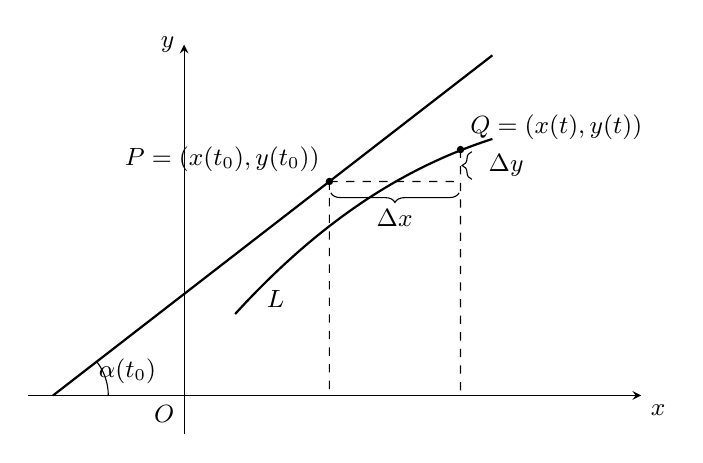
\begin{tikzpicture}[scale=0.9,>=stealth,font=\small]
  \draw[->] (-2.20,0) -- (6.45,0) node[below right] {$x$};
  \draw[->] (0,-0.55) -- (0,4.95) node[left] {$y$};
  \node[below left] at (0,0) {$O$};
  % 曲线 L
  \draw[thick] (0.72,1.15) .. controls (2.00,2.55) and (3.20,3.25) .. (4.35,3.62);
  \node[below left] at (1.55,1.62) {$L$};
  % 切线
  \draw[thick] (-1.85,0) -- (4.35,4.80);
  % P, Q
  \coordinate (P) at (2.05,3.02);
  \coordinate (Q) at (3.90,3.47);
  \fill (P) circle (1.5pt);
  \fill (Q) circle (1.5pt);
  \node[above left] at (P) {$P = (x(t_0), y(t_0))$};
  \node[above right] at (Q) {$Q = (x(t), y(t))$};
  % 虚线
  \draw[dashed] (P) -- (3.90,3.02);
  \draw[dashed] (P) -- (2.05,0);
  \draw[dashed] (Q) -- (3.90,0);
  % Delta x / Delta y
  \draw[decorate,decoration={brace,amplitude=3.5pt,mirror}] (2.07,2.86) -- (3.88,2.86);
  \node at (2.97,2.50) {$\Delta x$};
  \draw[decorate,decoration={brace,amplitude=3.5pt}] (4.06,3.05) -- (4.06,3.44);
  \node[right] at (4.16,3.24) {$\Delta y$};
  % 角 alpha(t0)
  \draw (-1.85,0) ++(0.78,0) arc (0:37.7:0.78);
  \node at (-0.80,0.34) {$\alpha(t_0)$};
\end{tikzpicture}
\caption{}\label{fig:3.2.1}
\end{figure}

如果 $x = x(t)$ 具有反函数 $t = t(x)$, 则
\[
y = y(t) = y(t(x)).
\]
这时只要 $x(t)$, $y(t)$ 可导, $x'(t) \neq 0$ (因而当 $\Delta x \to 0$ 时, 也有 $\Delta t \to 0$ 与 $\Delta y \to 0$), 就有
\[
\frac{\mathrm{d}y}{\mathrm{d}x} = \frac{\mathrm{d}y}{\mathrm{d}t}\cdot\frac{\mathrm{d}t}{\mathrm{d}x} = \frac{\mathrm{d}y}{\mathrm{d}t}\bigg/\frac{\mathrm{d}x}{\mathrm{d}t} = \frac{y'(t)}{x'(t)},\ \text{或}\ y'_{x} = \frac{y'_{t}}{x'_{t}}.
\]
如果 $x(t)$, $y(t)$ 均 2 阶可导, 则
\[
\begin{aligned}
\frac{\mathrm{d}^{2}y}{\mathrm{d}x^{2}} &= \frac{\mathrm{d}}{\mathrm{d}x}\left(\frac{\mathrm{d}y}{\mathrm{d}x}\right) = \frac{\left(\frac{y'(t)}{x'(t)}\right)'}{x'(t)} = \frac{y''(t)x'(t) - y'(t)x''(t)}{x'(t)[x'(t)]^{2}}\\
&= \frac{x'(t)y''(t) - y'(t)x''(t)}{[x'(t)]^{3}}.
\end{aligned}
\]
当曲线 $L$ 由极坐标方程 $\rho = \rho(\theta)$ 表示, 则可用极角 $\theta$ 作为参数, 即
\[
(x, y) = (\rho(\theta)\cos\theta, \rho(\theta)\sin\theta).
\]
如果 $\rho$ 可导, 则曲线 $\rho = \rho(\theta)$ 上点 $M(\rho, \theta)$ 处切线 $MT$ 与极轴 $Ox$ 轴的夹角 $\alpha$ 的正切(即切线斜率)为
\[
\begin{aligned}
\tan\alpha &= \frac{\mathrm{d}y}{\mathrm{d}x} = \frac{y'(\theta)}{x'(\theta)} = \frac{(\rho(\theta)\sin\theta)'}{(\rho(\theta)\cos\theta)'}\\
&= \frac{\rho'(\theta)\sin\theta + \rho(\theta)\cos\theta}{\rho'(\theta)\cos\theta - \rho(\theta)\sin\theta} = \frac{\rho'(\theta)\tan\theta + \rho(\theta)}{\rho'(\theta) - \rho(\theta)\tan\theta}.
\end{aligned}
\]
如图~\ref{fig:3.2.2} 所示, 过点 $M$ 的射线 $OH$ ($O$ 为极点, $Ox$ 为极轴) 与切线 $MT$ 的夹角 $\varphi$ 的正切为
\[
\begin{aligned}
\tan\varphi &= \tan(\alpha - \theta) = \frac{\tan\alpha - \tan\theta}{1 + \tan\alpha\tan\theta}\\
&= \frac{\frac{\rho'(\theta)\tan\theta + \rho(\theta)}{\rho'(\theta) - \rho(\theta)\tan\theta} - \tan\theta}{1 + \frac{\rho'(\theta)\tan\theta + \rho(\theta)}{\rho'(\theta) - \rho(\theta)\tan\theta}\tan\theta}\\
&= \frac{\rho'(\theta)\tan\theta + \rho(\theta) - \rho'(\theta)\tan\theta + \rho(\theta)\tan^{2}\theta}{\rho'(\theta) - \rho(\theta)\tan\theta + \rho'(\theta)\tan^{2}\theta + \rho(\theta)\tan\theta}\\
&= \frac{\rho(\theta)(1 + \tan^{2}\theta)}{\rho'(\theta)(1 + \tan^{2}\theta)} = \frac{\rho(\theta)}{\rho'(\theta)}.
\end{aligned}
\]

\begin{figure}[htbp]
\centering
\begin{tikzpicture}[scale=0.95,>=stealth,font=\small]
  \draw[->] (-1.05,0) -- (5.45,0) node[below right] {$x$};
  \node[below left] at (0,0) {$O$};
  % 射线 OH
  \draw[thick] (0,0) -- (5.00,3.29);
  \node[right] at (5.05,3.35) {$H$};
  % 角 theta
  \draw (0,0) ++(0.95,0) arc (0:33.3:0.95);
  \node at (0.98,0.30) {$\theta$};
  % 曲线
  \draw[thick] (1.86,1.02) .. controls (2.20,1.28) and (2.46,1.53) .. (2.507,1.647)
        .. controls (2.55,1.75) and (2.70,2.55) .. (2.86,3.30);
  % 切线 MT
  \draw[thick] (1.835,0) -- (3.86,4.96);
  \node[right] at (3.82,4.90) {$T$};
  % 点 M
  \fill (2.507,1.647) circle (1.6pt);
  \node[left] at (2.36,1.70) {$M$};
  % 角 alpha
  \draw (1.835,0) ++(0.65,0) arc (0:67.8:0.65);
  \node at (2.30,0.42) {$\alpha$};
  % 角 varphi
  \draw (2.507,1.647) ++(33.3:0.70) arc (33.3:67.8:0.70);
  \node at (3.11,2.38) {$\varphi$};
\end{tikzpicture}
\caption{}\label{fig:3.2.2}
\end{figure}

\begin{example}\label{ex:3.2.9}
证明: 对数螺线 $\rho = \mathrm{e}^{\frac{\theta}{2}}$ 上所有点的切线与向径的夹角 $\varphi$ 为常量.
\end{example}

\begin{proof}
因为
\[
\tan\varphi = \frac{\rho(\theta)}{\rho'(\theta)} = \frac{\mathrm{e}^{\frac{\theta}{2}}}{\frac{1}{2}\mathrm{e}^{\frac{\theta}{2}}} = 2,
\]
所以 $\varphi = \arctan 2$ 为常量.
\end{proof}

\begin{example}\label{ex:3.2.10}
求由上半椭圆的参数方程 $(x, y) = (a\cos t, b\sin t)$, $0 < t < \pi$ 所确定的函数 $y = y(x) = b\sqrt{1 - \frac{x^{2}}{a^{2}}}$ 的导数 $\frac{\mathrm{d}y}{\mathrm{d}x}$ 与 2 阶导数 $\frac{\mathrm{d}^{2}y}{\mathrm{d}x^{2}}$.
\end{example}

\begin{solution}
\[
\frac{\mathrm{d}y}{\mathrm{d}x} = \frac{\mathrm{d}y}{\mathrm{d}t}\bigg/\frac{\mathrm{d}x}{\mathrm{d}t} = \frac{b\cos t}{-a\sin t} = -\frac{b}{a}\cot t.
\]
\[
\frac{\mathrm{d}^{2}y}{\mathrm{d}x^{2}} = \frac{\mathrm{d}}{\mathrm{d}x}\left(\frac{\mathrm{d}y}{\mathrm{d}x}\right) = \frac{-\frac{b}{a}(\cot t)'}{-a\sin t} = \frac{-\frac{b}{a}(-\csc^{2}t)}{-a\sin t} = -\frac{b}{a^{2}\sin^{3}t}.
\]
或直接代入公式得到
\[
\begin{aligned}
\frac{\mathrm{d}^{2}y}{\mathrm{d}x^{2}} &= \frac{x'(t)y''(t) - y'(t)x''(t)}{[x'(t)]^{3}}\\
&= \frac{(-a\sin t)(-b\sin t) - (b\cos t)(-a\cos t)}{(-a\sin t)^{3}}\\
&= -\frac{b}{a^{2}\sin^{3}t}.
\end{aligned}
\]
请读者对 $y = b\sqrt{1 - \frac{x^{2}}{a^{2}}}$ 关于 $x$ 求 1 阶、2 阶导数来验证上述结果.
\end{solution}

\begin{example}\label{ex:3.2.11}
求由摆线参数方程 $(x, y) = (a(t - \sin t), a(1 - \cos t))$ 所确定的函数 $y = y(x)$ 的 2 阶导数.
\end{example}

\begin{solution}
\[
\frac{\mathrm{d}y}{\mathrm{d}x} = \frac{y'(t)}{x'(t)} = \frac{a\sin t}{a(1 - \cos t)} = \frac{2\sin\frac{t}{2}\cos\frac{t}{2}}{2\sin^{2}\frac{t}{2}} = \cot\frac{t}{2},
\]
\[
\frac{\mathrm{d}^{2}y}{\mathrm{d}x^{2}} = \frac{\mathrm{d}}{\mathrm{d}x}\left(\frac{\mathrm{d}y}{\mathrm{d}x}\right) = \frac{\left(\cot\frac{t}{2}\right)'}{a(1 - \cos t)} = \frac{-\frac{1}{2}\csc^{2}\frac{t}{2}}{2a\sin^{2}\frac{t}{2}} = -\frac{1}{4a}\csc^{4}\frac{t}{2}.
\]
\end{solution}

\begin{example}\label{ex:3.2.12}
设曲线参数方程为 $(x, y) = (1 - t^{2}, t - t^{2})$, 求它在 $t = 1$ 处的切线方程与法线方程.
\end{example}

\begin{solution}
因为
\[
\frac{\mathrm{d}y}{\mathrm{d}x}\bigg|_{t=1} = \frac{y'_{t}}{x'_{t}}\bigg|_{t=1} = \frac{1 - 2t}{-2t}\bigg|_{t=1} = \frac{1}{2},
\]
故切线方程为 $y - 0 = \frac{1}{2}(x - 0)$, 即 $y = \frac{1}{2}x$; 法线方程为 $y - 0 = -2(x - 0)$, 即 $y = -2x$.
\end{solution}

\begin{remark}\label{rem:3.2.2}
加速度是位移 $x(t)$ 对时间 $t$ 的 2 阶导数, 这是高阶导数在物理中的应用. 在古典微分几何中, 考虑 2 阶连续可导的正则曲线 $(x(t), y(t))$, 所谓正则指的是 $(x'(t))^{2} + (y'(t))^{2} \neq 0$, 从反映它弯曲程度的曲率公式
\[
\kappa(t) = \frac{x'(t)y''(t) - x''(t)y'(t)}{\left[(x'(t))^{2} + (y'(t))^{2}\right]^{3/2}},
\]
可看出 2 阶导数在几何中的重要应用. 在 3.6 节, 我们还可用 2 阶导数来刻画曲线的凹凸性与拐点以及判断函数的驻点(即 1 阶导数为 0 的点)是否为极值点, 是极大值点还是极小值点.
\end{remark}

\begin{exblock}{练习题 3.2}
  \item 求 $y$ 关于 $x$ 的 2 阶导数 $y''$.
  \begin{enumerate}[label=(\arabic*)]
    \item $y = \mathrm{e}^{-x^{2}}$;
    \item $y = x^{2}a^{x}$ ($a > 0$);
    \item $y = \ln\sin x$;
    \item $y = (1 + x^{2})\arctan x$;
    \item $y = \frac{\arcsin x}{\sqrt{1 - x^{2}}}$;
    \item $y = x\ln x$.
  \end{enumerate}

  \item 
  \begin{enumerate}[label=(\arabic*)]
    \item 设 $f(x) = \mathrm{e}^{2x-1}$, 求 $f''(0)$;
    \item 设 $f(x) = \arctan x$, 求 $f''(1)$;
    \item 设 $f(x) = \sin^{2}x$, 求 $f''\left(\frac{\pi}{2}\right)$;
    \item 设 $f(x) = 3x^{3} + 4x^{2} - 5x - 9$, 求 $f''(1)$, $f'''(1)$, $f^{(4)}(1)$.
  \end{enumerate}

  \item 求下列高阶导数:
  \begin{enumerate}[label=(\arabic*)]
    \item $f(x) = \frac{1+x}{\sqrt{1-x}}$, 求 $f^{(10)}(x)$;
    \item $f(x) = \frac{x^{2}}{1-x}$, 求 $f^{(8)}(x)$;
    \item $f(x) = \mathrm{e}^{-x^{2}}$, 求 $f''(x)$;
    \item $f(x) = \ln(1+x)$, 求 $f^{(5)}(x)$;
    \item $f(x) = x^{3}\mathrm{e}^{x}$, 求 $f^{(10)}(x)$.
  \end{enumerate}

  \item 设函数 $f$ 在 $(-\infty, x_0]$ 上 2 阶可导,
  \[
  F(x) = \begin{cases}f(x), & x \leqslant x_0,\\ a(x-x_0)^{2} + b(x-x_0) + c, & x > x_0.\end{cases}
\]
  问: 当 $a$, $b$, $c$ 为何值时函数 $F$ 在 $\mathbb{R}$ 上有 2 阶导函数.

  \item 设 $f$ 为 2 阶可导函数, 求下列各函数的 2 阶导函数.
  \begin{enumerate}[label=(\arabic*)]
    \item $y = f(\ln x)$;
    \item $y = f(x^{n})$, $n \in \mathbb{N}$;
    \item $y = f(f(x))$.
  \end{enumerate}

  \item 设函数 $f$ 在点 $x = 1$ 处 2 阶可导, $f'(1) = 0$, $f''(1) = 0$. 证明: 在 $x = 1$ 处有
  \[
  \frac{\mathrm{d}}{\mathrm{d}x}f(x^{2}) = \frac{\mathrm{d}^{2}}{\mathrm{d}x^{2}}f^{2}(x).
\]

  \item 求下列函数的 $n$ 阶导数:
  \begin{enumerate}[label=(\arabic*)]
    \item $y = \ln x$;
    \item $y = \frac{\ln x}{x}$;
    \item $y = \frac{1}{x(1-x)}$;
    \item $f(x) = \frac{x^{n}}{1-x}$;
    \item $v = \mathrm{e}^{ax}\sin bx$ ($a$, $b$ 均为实数).
  \end{enumerate}

  \item 设 $y = \frac{ax+b}{cx+d}$. 证明:
  \[
  y^{(n)}(x) = (-1)^{n+1}\frac{n!\,c^{n-1}}{(cx+d)^{n+1}}\begin{vmatrix}a & b\\ c & d\end{vmatrix}.
\]

  \item 证明: 函数
  \[
  f(x) = \begin{cases}\mathrm{e}^{-\frac{1}{x^{2}}}, & x \neq 0,\\ 0, & x = 0\end{cases}
\]
  在 $x = 0$ 处 $n$ 阶可导, 且 $f^{(n)}(0) = 0$, 其中 $n \in \mathbb{N}$.

  \item 求由下列参数方程所确定的函数的 2 阶导数 $\frac{\mathrm{d}^{2}y}{\mathrm{d}x^{2}}$:
  \begin{enumerate}[label=(\arabic*)]
    \item $\begin{cases}x = a\cos^{3}t,\\ y = a\sin^{3}t;\end{cases}$
    \item $\begin{cases}x = \mathrm{e}^{t}\cos t,\\ y = \mathrm{e}^{t}\sin t;\end{cases}$
    \item $\begin{cases}x = \cos^{4}t,\\ y = \sin^{4}t;\end{cases}$
    \item $\begin{cases}x = \frac{t}{1+t},\\ y = \frac{1-t}{1+t}.\end{cases}$
  \end{enumerate}

  \item 证明: 原点到曲线
  \[
  \begin{cases}x = a(\cos t + t\sin t),\\ y = a(\sin t - t\cos t)\end{cases}
\]
  上任一点的法线的距离等于 $a$.

  \item 证明: 圆 $r = 2a\sin\theta$ ($a > 0$) 上任一点的切线与向径的夹角等于向径的极角.

  \item 求心形(脏)线 $r = a(1 + \cos\theta)$ 的切线与切点向径之间的夹角.
\end{exblock}

\begin{exblock}{思考题 3.2}
  \item 设 $m$, $n \in \mathbb{N}$. 证明:
  \[
  \sum_{k=0}^{n}(-1)^{k}\mathrm{C}_{n}^{k}k^{m} = \begin{cases}0, & m \leqslant n-1,\\ (-1)^{n}n!, & m = n.\end{cases}
\]

  \item 设 $u$, $v$, $w$ 都为 $t$ 的可导函数. 试给出 $(uvw)^{(n)}$ 的 Leibniz 公式, 这里 $n \in \mathbb{N}$.

  \item 设 $y = x^{n-1}\mathrm{e}^{\frac{1}{x}}$. 证明:
  \[
  y^{(n)} = \frac{(-1)^{n}}{x^{n+1}}\mathrm{e}^{\frac{1}{x}}.
\]

  \item 设 $y = \arctan x$. 证明:
  \[
  y^{(n)} = \frac{P_{n-1}(x)}{(1+x^{2})^{n}},
\]
  其中 $P_{n-1}$ 为最高次项系数是 $(-1)^{n-1}n!$ 的 $n-1$ 次多项式.

  \item 设 $f(x) = x^{n}\ln x$, $n \in \mathbb{N}$, 求极限
  \[
  \lim_{n\to+\infty}\frac{f^{(n)}\left(\frac{1}{n}\right)}{n!}.
\]

  \item 证明: 在 $\mathbb{R}$ 上不存在可导函数 $f$ 满足 $f^{2}(x) = -x^{3} + x^{2} + 1$.

  \item 证明: 在 $\mathbb{R}$ 上不存在可导函数 $f$ 满足 $f^{2}(x) = x^{2} - 3x + 3$.

  \item 求 $\left(\mathrm{e}^{x}\cos x\right)^{(n)}$ 与 $\left(\mathrm{e}^{x}\sin x\right)^{(n)}$.

  \item 设 $y = (1 + \sqrt{x})^{2n+2}$, $n \in \mathbb{N}$, 求 $y^{(n)}(1)$.

  \item 设多项式 $p$ 只有实零点, 证明: $(p'(x))^{2} \geqslant p(x)p''(x)$ 对一切 $x \in \mathbb{R}$ 成立.

  \item 设 $y = \arctan x$.
  \begin{enumerate}[label=(\arabic*)]
    \item 证明它满足方程 $(1+x^{2})y'' + 2xy' = 0$;
    \item 求 $y^{(n)}(0)$.
  \end{enumerate}

  \item 设 $f(x) = \arctan x$. 证明:
  \[
  f^{(n)}(x) = (n-1)!\cos^{n}f(x)\cdot\sin\left(f(x) + \frac{n\pi}{2}\right).
\]
\end{exblock}

% ====================================================================
%  徐森林、薛春华《数学分析》（第一册）
%  \S3.3  微分中值定理
%  源：原书印刷页 185-198（PDF 物理页 191-204）
%  底本：PaddleOCR-VL-1.6 + 高清影印比对校订
%  规范：全西文半角标点；单一落盘出口 _texout.py
% ====================================================================
\section{微分中值定理}\label{sec:3.3}

这一节主要讨论微分学中重要的 Fermat 定理、Rolle 定理、Lagrange 中值定理以及 Cauchy 中值定理, 它们是研究函数的增减性、凹凸性、极值与最值的基础.

\begin{definition}\label{def:3.3.1}
设 $f$ 定义在区间 $I$ 上, $x_0$ 为 $I$ 的内点, 即 $\exists\delta_0>0$, s.t. $B(x_0;\delta_0)=(x_0-\delta,x_0+\delta)\subset I$. 如果 $x_0$ 有一个开邻域 $B(x_0;\delta)=(x_0-\delta,x_0+\delta)\subset I$, s.t. $f(x_0)$ 为 $f(x)$ 在 $(x_0-\delta,x_0+\delta)$ 中的最大(小)值, 即 $f(x)\leqslant f(x_0)$ ($f(x)\geqslant f(x_0)$), 则称 $f(x_0)$ 为 $f$ 的极大(小)值, $x_0$ 称为 $f$ 的极大(小)值点. 极大值与极小值统称为极值. 极大值点与极小值点统称为极值点.
\end{definition}

如果 $x_0$ 为 $I$ 中的内点, 且为 $f$ 的最大(小)值点, 显然, $x_0$ 为 $f$ 的极大(小)值点. 但是, 反之不一定成立. 例如:
\[
f(x)=\begin{cases}x+1,&-2<x\leqslant0,\\ -x+1,&0<x\leqslant1,\\ 2x-2,&1<x\leqslant2,\end{cases}
\]
$x=0$ 为极大值点但非最大值点, $x=1$ 为极小值点但非最小值点.

注意, 最大(小)值若在区间端点达到, 则它就不是极大(小)值.

极值是局部性质, 而最值是整体性质.

\begin{theorem}[Fermat (1601---1665) 定理]\label{thm:3.3.1}
设 $f$ 在点 $x_0$ 处可导, $x_0$ 为 $f$ 的极值点, 则 $f'(x_0)=0$. 但反之不一定成立.
\end{theorem}

若 $f'(x_0)=0$, 则 $x_0$ 称为 $f$ 的驻点或稳定点.

\begin{proof}
不妨设 $x_0$ 为 $f$ 的极大值点, 即 $\exists\delta>0$, s.t. $f(x)\leqslant f(x_0)$, $\forall x\in(x_0-\delta,x_0+\delta)$. 于是(如图~\ref{fig:3.3.1} 所示),
\[
\frac{f(x)-f(x_0)}{x-x_0}\begin{cases}\geqslant0,&x_0-\delta<x<x_0,\\ \leqslant0,&x_0<x<x_0+\delta.\end{cases}
\]
又因为 $f$ 在点 $x_0$ 处可导, 故
\[
\begin{aligned}
0 &\leqslant\lim_{x\to x_0^-}\frac{f(x)-f(x_0)}{x-x_0}=f'_-(x_0)=f'(x_0)=f'_+(x_0)\\
&=\lim_{x\to x_0^+}\frac{f(x)-f(x_0)}{x-x_0}\leqslant0,
\end{aligned}
\]
\[
f'(x_0)=0.
\]
\end{proof}

建议读者用反证法证明 $f'(x_0)=0$.

反之有反例: $f(x)=x^{3}$, $f'(x)=3x^{2}$, $f'(0)=0$, $0$ 为 $f$ 的驻点, 但由 $f$ 严格增与反证法知, $0$ 不是 $f$ 的极值点.

\begin{remark}\label{rem:3.3.1}
定理~\ref{thm:3.3.1} 中, “可导”条件不能删去.

反例: $y=f(x)=|x|$, 显然 $0$ 为 $f$ 的极小值点(也是最小值点), 但由于 $f$ 在点 $0$ 处不可导, 当然谈不上 $f'(0)=0$.
\end{remark}

\begin{figure}[htbp]
\centering
\begin{tikzpicture}[scale=1.0,>=stealth,font=\small]
  \draw[->] (-1.60,0) -- (6.55,0) node[below right] {$x$};
  \draw[->] (0,-0.85) -- (0,5.70) node[left] {$y$};
  \node[below left] at (0,0) {$O$};
  % 水平切线 y = f(x_0)
  \draw[thick] (-1.25,3.30) -- (4.80,3.30);
  \node[left] at (-1.28,3.30) {$f(x_0)$};
  % 曲线 y = f(x)
  \draw[thick] (0.94,1.88) .. controls (1.55,2.42) and (2.35,3.23) .. (3.06,3.23)
               .. controls (3.85,3.23) and (4.72,2.52) .. (5.61,1.84);
  % 三条竖直虚线
  \draw[dashed] (1.33,3.30) -- (1.33,-1.12);
  \draw[dashed] (2.99,3.30) -- (2.99,-1.12);
  \draw[dashed] (4.80,3.30) -- (4.80,-0.52);
  % 横轴标签
  \node[below] at (1.33,-1.16) {$x_0-\delta$};
  \node[below] at (2.99,-1.16) {$x_0$};
  \node[below] at (4.80,-0.56) {$x_0+\delta$};
\end{tikzpicture}
\caption{}\label{fig:3.3.1}
\end{figure}

\begin{theorem}[Rolle (1652---1719) 定理]\label{thm:3.3.2}
设 $f$ 在 $[a,b]$ 上连续, 在 $(a,b)$ 内可导, $f(a)=f(b)$, 则 $\exists\xi\in(a,b)$, s.t. $f'(\xi)=0$ (即 $(\xi,f(\xi))$ 或 $\xi$ 点处的切线平行于 $x$ 轴, 也平行于 $(a,f(a))$ 与 $(b,f(b))$ 的连线).
\end{theorem}

\begin{proof}
因为 $f$ 在 $[a,b]$ 上连续, 由最值定理知, $f$ 必达到最大值与最小值, 即 $\exists\alpha,\beta\in[a,b]$, s.t. $f(\alpha)\leqslant f(x)\leqslant f(\beta)$, $\forall x\in[a,b]$.

如果 $\alpha,\beta\in\{a,b\}$, 则由 $f(a)=f(b)$ 知, $f(x)=f(a)=f(b)$, $\forall x\in[a,b]$, 即 $f$ 为 $[a,b]$ 上的常值函数. 于是, $\forall\xi\in(a,b)$, $f'(\xi)=0$.

如果 $\alpha,\beta$ 中有一个不是端点, 例如 $\alpha\in(a,b)$, 则由 $f$ 在 $\alpha$ 达到最小值, 它必为极小值, 由 Fermat 定理知, $f'(\alpha)=0$. 因此, $\xi=\alpha$ 为定理所求之点.
\end{proof}

\begin{theorem}[Lagrange (1736---1813) 中值定理]\label{thm:3.3.3}
设 $f$ 在 $[a,b]$ 上连续, 在 $(a,b)$ 内可导, 则 $\exists\xi\in(a,b)$, s.t.
\[
f'(\xi)=\frac{f(b)-f(a)}{b-a}
\]
($(\xi,f(\xi))$ 点处的切线平行 $(a,f(a))$ 与 $(b,f(b))$ 的连线) 或
\[
\begin{aligned}
f(b)-f(a)&=f'(\xi)(b-a)\\
&=f'[a+\theta(b-a)](b-a),
\end{aligned}
\]
其中 $0<\theta=\frac{\xi-a}{b-a}<1$.
\end{theorem}

\begin{figure}[htbp]
\centering
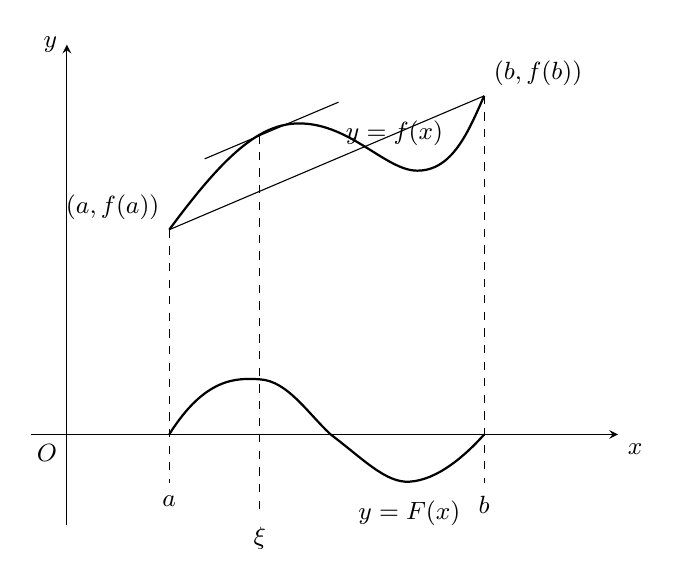
\begin{tikzpicture}[scale=1.0,>=stealth,font=\small]
  \draw[->] (-0.45,0) -- (7.00,0) node[below right] {$x$};
  \draw[->] (0,-1.15) -- (0,4.95) node[left] {$y$};
  \node[below left] at (0,0) {$O$};
  % 曲线 y = f(x)
  \draw[thick] (1.30,2.60) .. controls (2.00,3.55) and (2.45,3.95) .. (2.95,3.95)
               .. controls (3.60,3.95) and (4.05,3.35) .. (4.45,3.35)
               .. controls (4.90,3.35) and (5.10,3.85) .. (5.30,4.30);
  % 弦 (a,f(a)) -- (b,f(b))
  \draw (1.30,2.60) -- (5.30,4.30);
  % 平行于弦的切线 (过 xi 处切点)
  \draw (1.75,3.50) -- (3.45,4.22);
  % 辅助函数 y = F(x)
  \draw[thick] (1.30,0) .. controls (1.75,0.72) and (2.15,0.72) .. (2.45,0.70)
               .. controls (2.80,0.68) and (3.05,0.28) .. (3.35,0.00)
               .. controls (3.75,-0.30) and (4.05,-0.62) .. (4.35,-0.60)
               .. controls (4.70,-0.58) and (5.05,-0.28) .. (5.30,0.00);
  % 三条竖直虚线
  \draw[dashed] (1.30,2.60) -- (1.30,-0.62);
  \draw[dashed] (2.45,3.80) -- (2.45,-1.02);
  \draw[dashed] (5.30,4.30) -- (5.30,-0.62);
  % 标注
  \node[above left] at (1.30,2.60) {$(a,f(a))$};
  \node[above right] at (5.30,4.30) {$(b,f(b))$};
  \node[right] at (3.42,3.82) {$y=f(x)$};
  \node[below] at (4.35,-0.72) {$y=F(x)$};
  \node[below] at (1.30,-0.66) {$a$};
  \node[below] at (2.45,-1.06) {$\xi$};
  \node[below] at (5.30,-0.66) {$b$};
\end{tikzpicture}
\caption{}\label{fig:3.3.2}
\end{figure}

当 $f(a)=f(b)$ 时, $f'(\xi)=\frac{f(b)-f(a)}{b-a}=0$. 因此, Lagrange 中值定理为 Rolle 定理的推广.

\begin{proof}[证法 1]
从图~\ref{fig:3.3.2} 想到令
\[
F(x)=f(x)-\left[f(a)+\frac{f(b)-f(a)}{b-a}(x-a)\right],
\]
则由 $f$ 在 $[a,b]$ 上连续, 在 $(a,b)$ 上可导知, $F$ 在 $[a,b]$ 上连续, 在 $(a,b)$ 上可导, 且
\[
\begin{aligned}
F(a)&=f(a)-\left[f(a)+\frac{f(b)-f(a)}{b-a}(a-a)\right]=0\\
&=f(b)-\left[f(a)+\frac{f(b)-f(a)}{b-a}(b-a)\right]=F(b).
\end{aligned}
\]
根据 Rolle 定理可得, $\exists\xi\in(a,b)$, s.t.
\[
0=F'(\xi)=f'(\xi)-\frac{f(b)-f(a)}{b-a},
\]
\[
f'(\xi)=\frac{f(b)-f(a)}{b-a}.
\]
\end{proof}

\begin{proof}[证法 2]
令
\[
\begin{aligned}
F(x)&=\begin{vmatrix}1&a&f(a)\\1&b&f(b)\\1&x&f(x)\end{vmatrix}=\begin{vmatrix}1&a&f(a)\\0&b-a&f(b)-f(a)\\0&x-a&f(x)-f(a)\end{vmatrix}\\
&=(b-a)[f(x)-f(a)]-(x-a)[f(b)-f(a)],
\end{aligned}
\]
则由 $f$ 在 $[a,b]$ 上连续, 在 $(a,b)$ 内可导知, $F$ 在 $[a,b]$ 上连续, 在 $(a,b)$ 内可导, 且
\[
F(a)=\begin{vmatrix}1&a&f(a)\\1&b&f(b)\\1&a&f(a)\end{vmatrix}=0=\begin{vmatrix}1&a&f(a)\\1&b&f(b)\\1&b&f(b)\end{vmatrix}=F(b).
\]
根据 Rolle 定理知, $\exists\xi\in(a,b)$, s.t.
\[
\begin{aligned}
0=F'(\xi)&=\begin{vmatrix}1&a&f(a)\\1&b&f(b)\\0&1&f'(x)\end{vmatrix}_{x=\xi}=\begin{vmatrix}1&a&f(a)\\0&b-a&f(b)-f(a)\\0&1&f'(\xi)\end{vmatrix}\\
&=(b-a)f'(\xi)-[f(b)-f(a)],
\end{aligned}
\]
\[
f'(\xi)=\frac{f(b)-f(a)}{b-a}.
\]
\end{proof}

\begin{theorem}[Cauchy (1789---1957) 中值定理]\label{thm:3.3.4}
设 $f$, $g$ 在 $[a,b]$ 上连续, 在 $(a,b)$ 内可导, 且 $g'(x)\neq0$, $\forall x\in(a,b)$, 则 $\exists\xi\in(a,b)$, s.t.
\[
\frac{f(b)-f(a)}{g(b)-g(a)}=\frac{f'(\xi)}{g'(\xi)}.
\]
\end{theorem}

特别地, 当 $g(x)=x$ 时, 它就是 Lagrange 中值定理. 因此, Cauchy 中值定理为 Lagrange 中值定理的推广.

\begin{proof}[证法 1]
先证 $g(b)\neq g(a)$.

用反证法. 假设 $g(b)=g(a)$, 由 Rolle 定理知, $\exists\eta\in(a,b)$, s.t. $g'(\eta)=0$, 这与 $g'(x)\neq0$, $\forall x\in(a,b)$ 矛盾. 或由 Lagrange 中值定理知, $\exists\eta\in(a,b)$, s.t. $g(b)-g(a)=g'(\eta)(b-a)\neq0$, 故 $g(b)\neq g(a)$.

仿照定理~\ref{thm:3.3.3} 证法 1, 令
\[
F(x)=f(x)-\left[f(a)+\frac{f(b)-f(a)}{g(b)-g(a)}(g(x)-g(a))\right],
\]
则由 $f$, $g$ 在 $[a,b]$ 上连续, 在 $(a,b)$ 内可导知 $F$ 在 $[a,b]$ 上连续, 在 $(a,b)$ 内可导, 且
\[
\begin{aligned}
F(a)&=f(a)-\left[f(a)+\frac{f(b)-f(a)}{g(b)-g(a)}(g(a)-g(a))\right]=0\\
&=f(b)-\left[f(a)+\frac{f(b)-f(a)}{g(b)-g(a)}(g(b)-g(a))\right]\\
&=F(b).
\end{aligned}
\]
根据 Rolle 定理可得, $\exists\xi\in(a,b)$, s.t.
\[
0=F'(\xi)=f'(\xi)-\frac{f(b)-f(a)}{g(b)-g(a)}g'(\xi),
\]
\[
\frac{f(b)-f(a)}{g(b)-g(a)}=\frac{f'(\xi)}{g'(\xi)}.
\]
\end{proof}

\begin{proof}[证法 2]
仿照定理~\ref{thm:3.3.3} 证法 2, 令
\[
F(x)=\begin{vmatrix}1&g(a)&f(a)\\1&g(b)&f(b)\\1&g(x)&f(x)\end{vmatrix},
\]
则由 $f$, $g$ 在 $[a,b]$ 上连续, 在 $(a,b)$ 内可导知, $F$ 在 $[a,b]$ 上连续, 在 $(a,b)$ 内可导, 且
\[
F(a)=\begin{vmatrix}1&g(a)&f(a)\\1&g(b)&f(b)\\1&g(a)&f(a)\end{vmatrix}=0=\begin{vmatrix}1&g(a)&f(a)\\1&g(b)&f(b)\\1&g(b)&f(b)\end{vmatrix}=F(b).
\]
根据 Rolle 定理可得, $\exists\xi\in(a,b)$, s.t.
\[
\begin{aligned}
0=F'(\xi)&=\begin{vmatrix}1&g(a)&f(a)\\1&g(b)&f(b)\\0&g'(x)&f'(x)\end{vmatrix}_{x=\xi}=\begin{vmatrix}1&g(a)&f(a)\\0&g(b)-g(a)&f(b)-f(a)\\0&g'(\xi)&f'(\xi)\end{vmatrix}\\
&=f'(\xi)[g(b)-g(a)]-g'(\xi)[f(b)-f(a)],
\end{aligned}
\]
\[
\frac{f(b)-f(a)}{g(b)-g(a)}=\frac{f'(\xi)}{g'(\xi)}.
\]
\end{proof}

\begin{corollary}\label{cor:3.3.1}
设 $f$ 在区间 $I$ 上连续, 在 $\mathring{I}$ 内可导, 则
\[
f(x)=c\ (\text{常数})\Longleftrightarrow f'(x)=0,\quad\forall x\in\mathring{I}.
\]
\end{corollary}

\begin{proof}
($\Rightarrow$) 设 $f(x)=c$, $\forall x\in\mathring{I}$, 则 $f'(x)=c'=0$.

($\Leftarrow$) $\forall x_1,x_2\in I$, $x_1<x_2$, 由 $f$ 在 $[x_1,x_2]$ 上连续, 在 $(x_1,x_2)$ 内可导, 以及 Lagrange 中值定理可知, $\exists\xi\in(x_1,x_2)\subset\mathring{I}$, s.t.
\[
\begin{aligned}
f(x_2)-f(x_1)&=f'(\xi)(x_2-x_1)=0\cdot(x_2-x_1)=0,\\
f(x_1)&=f(x_2).
\end{aligned}
\]
因为 $x_1$, $x_2$ 是任取的, 所以, $f(x)=c$ (常数).
\end{proof}

\begin{example}\label{ex:3.3.1}
设
\[
f(x)=\begin{cases}1,&x>0,\\ -1,&x<0.\end{cases}
\]
显然, $f'(x)=0$, 但 $f(x)\neq c$ (常数). 注意: $f$ 的定义域不为一个区间. 因而, 推论~\ref{cor:3.3.1} 充分性的证明中不能应用 Lagrange 中值定理.
\end{example}

\begin{corollary}\label{cor:3.3.2}
设 $f$, $g$ 在区间 $I$ 上的连续, 在 $\mathring{I}$ 内可导, 则
\[
f(x)=g(x)+c\Longleftrightarrow f'(x)=g'(x),\quad\forall x\in\mathring{I},
\]
其中 $c$ 为常数.
\end{corollary}

\begin{proof}
\[
\begin{aligned}
& f(x)=g(x)+c,\ \forall x\in I\\
\Longleftrightarrow\ & f(x)-g(x)=c,\ \forall x\in I\\
\xlongleftrightarrow{\text{推论}~\ref{cor:3.3.1}}\ & f'(x)-g'(x)=[f(x)-g(x)]'=0,\ \forall x\in\mathring{I}\\
\Longleftrightarrow\ & f'(x)=g'(x),\ \forall x\in\mathring{I}.
\end{aligned}
\]
\end{proof}

\begin{corollary}\label{cor:3.3.3}
设 $I_1$, $I_2$ 为两个不相交的非空区间. 则
\[
f(x)=\begin{cases}g(x)+c_1,&x\in I_1,\\ g(x)+c_2,&x\in I_2,\end{cases}\qquad c_1\ \text{与}\ c_2\ \text{为两个无关的常数}
\]
\[
\Longleftrightarrow f'(x)=g'(x),\quad\forall x\in\mathring{I}_1\cup\mathring{I}_2.
\]
\end{corollary}

\begin{proof}
($\Rightarrow$) 显然.

($\Leftarrow$) 因 $f'(x)=g'(x)$, $\forall x\in\mathring{I}_1\cup\mathring{I}_2$, 根据推论~\ref{cor:3.3.1} 知, $\exists c_1,c_2\in\mathbb{R}$, s.t.
\[
f(x)=\begin{cases}g(x)+c_1,&x\in I_1,\\ g(x)+c_2,&x\in I_2.\end{cases}
\]
\end{proof}

\begin{theorem}[Darboux (1842---1917) 导函数介值定理]\label{thm:3.3.5}
设 $f$ 在 $[a,b]$ 内可导, 则对于 $f'_+(a)$ 与 $f'_-(b)$ 之间的一切值 $k$, 必有 $\xi\in[a,b]$, s.t. $f'(\xi)=k$.
\end{theorem}

如果 $f'_+(a)\neq f'_-(b)$, $k\in(\min\{f'_+(a),f'_-(a)\},\max\{f'_+(a),f'_-(a)\})$, 则可取 $\xi\in(a,b)$, s.t. $f'(\xi)=k$.

\begin{proof}[证法 1]
设 $F(x)=f(x)-kx$, 由 $f$ 在 $[a,b]$ 上可导知, $F$ 在 $[a,b]$ 上也可导, 且
\[
F'_+(a)\cdot F'_-(b)=(f'_+(a)-k)(f'_-(b)-k)\leqslant0.
\]
如果 $F'_+(a)\cdot F'_-(b)=0$, 则 $F'_+(a)=0$ 或 $F'_-(b)=0$, 取 $\xi=a$ 或 $b$.

如果 $F'_+(a)\cdot F'_-(b)<0$, 不妨设
\[
\lim_{x\to a^+}\frac{F(x)-F(a)}{x-a}=F'_+(a)>0,
\]
\[
\lim_{x\to b^-}\frac{F(x)-F(b)}{x-b}=F'_-(b)<0,
\]
由保号性定理知, $\exists a_1,b_1$, s.t. $a<a_1<b_1<b$, 且
\[
F(a)<F(a_1),\quad F(b_1)>F(b).\tag*{(*)}
\]
因为 $F$ 在 $[a,b]$ 上可导, 所以它在 $[a,b]$ 上连续. 根据最值定理知, $\exists\xi\in[a,b]$, s.t. $F$ 在 $\xi$ 达到最大值. 由 $(*)$ 式知, $\xi\neq a,b$, 必有 $\xi\in(a,b)$. 因此, $\xi$ 为 $F$ 的极大值点. 再根据 Fermat 定理得到
\[
\begin{aligned}
0=F'(\xi)&=(f(x)-kx)'\big|_{x=\xi}=f'(\xi)-k,\\
f'(\xi)&=k.
\end{aligned}
\]
\end{proof}

\begin{proof}[证法 2]
设
\[
\varphi_1(x)=\begin{cases}\frac{f(x)-f(a)}{x-a},&a<x\leqslant b,\\ f'_+(a),&x=a,\end{cases}
\]
\[
\varphi_2(x)=\begin{cases}\frac{f(x)-f(b)}{x-b},&a\leqslant x<b,\\ f'_-(b),&x=b.\end{cases}
\]
因为
\[
\lim_{x\to a^+}\varphi_1(x)=\lim_{x\to a^+}\frac{f(x)-f(a)}{x-a}=f'_+(a)=\varphi_1(a),
\]
\[
\lim_{x\to b^-}\varphi_2(x)=\lim_{x\to b^-}\frac{f(x)-f(b)}{x-b}=f'_-(b)=\varphi_2(b),
\]
所以, $\varphi_1$, $\varphi_2$ 都在 $[a,b]$ 上连续, 在 $(a,b)$ 内可导.

如果 $k=f'_+(a)$, 取 $\xi=a$; 如果 $k=f'_-(b)$, 取 $\xi=b$. 如果 $f'_+(a)<k<f'_-(b)$ (或 $f'_-(b)<k<f'_+(a)$), 则 $k$ 应介于 $f'_+(a)$ 与 $\frac{f(b)-f(a)}{b-a}$ 之间或介于 $\frac{f(b)-f(a)}{b-a}$ 与 $f'_-(b)$ 之间, 不妨设为前者. 由 $\varphi_1$ 的定义知, $k$ 介于 $\varphi_1(a)$ 与 $\varphi_1(b)$ 之间. 根据 $\varphi_1$ 的连续性及连续函数的介值定理知, $\exists\theta\in[a,b]$, 由 Lagrange 中值定理知, $\exists\xi\in(a,\theta)\subset(a,b)$, s.t.
\[
k=\varphi_1(\theta)=\frac{f(\theta)-f(a)}{\theta-a}=f'(\xi).
\]
\end{proof}

\begin{remark}\label{rem:3.3.2}
注意, Darboux 定理~\ref{thm:3.3.5} 中, $f'(x)$ 不必连续. 如果 $f'$ 连续, 只需将连续函数的介值定理应用于 $f'(x)$ 即得定理~\ref{thm:3.3.5} 的结论.
\end{remark}

\begin{example}\label{ex:3.3.2}
证明: $\forall h>-1$, $h\neq0$ 成立不等式
\[
\frac{h}{1+h}<\ln(1+h)<h.
\]
\end{example}

\begin{proof}
令 $f(x)=\ln(1+x)$, 则由 Lagrange 中值定理, 有
\[
\ln(1+h)=\ln(1+h)-\ln1=\frac{h}{1+\theta h},\quad0<\theta<1.
\]
如果 $h>0$, 由 $0<\theta<1$ 推得
\[
1<1+\theta h<1+h,
\]
\[
\frac{h}{1+h}<\frac{h}{1+\theta h}<h,
\]
\[
\frac{h}{1+h}<\ln(1+h)<h.
\]
如果 $-1<h<0$, 由 $0<\theta<1$ 推得
\[
0<1+h<1+\theta h<1,
\]
\[
\frac{h}{1+h}<\frac{h}{1+\theta h}<h,
\]
\[
\frac{h}{1+h}<\ln(1+h)<h.
\]
\end{proof}

\begin{example}\label{ex:3.3.3}
设 $0<\alpha\leqslant\beta<\frac{\pi}{2}$, 证明:
\[
\frac{\beta-\alpha}{\cos^{2}\alpha}\leqslant\tan\beta-\tan\alpha\leqslant\frac{\beta-\alpha}{\cos^{2}\beta}.
\]
\end{example}

\begin{proof}
当 $\alpha=\beta$ 时, 上述不等式为等式.

当 $\alpha\neq\beta$ 时, 令 $f(x)=\tan x$, $0<\alpha\leqslant x\leqslant\beta<\frac{\pi}{2}$. 由于 $f(x)=\tan x$ 在 $[\alpha,\beta]$ 上连续, 在 $(\alpha,\beta)$ 内可导, 根据 Lagrange 中值定理知, $\exists\xi\in(\alpha,\beta)$, s.t. $\tan\beta-\tan\alpha=(\tan x)'\big|_{x=\xi}(\beta-\alpha)=\sec^{2}\xi\cdot(\beta-\alpha)=\frac{\beta-\alpha}{\cos^{2}\xi}$. 于是,
\[
\begin{aligned}
&\frac{\beta-\alpha}{\cos^{2}\alpha}<\frac{\beta-\alpha}{\cos^{2}\xi}<\frac{\beta-\alpha}{\cos^{2}\beta}.\\
&\frac{\beta-\alpha}{\cos^{2}\alpha}<\tan\beta-\tan\alpha<\frac{\beta-\alpha}{\cos^{2}\beta}.
\end{aligned}
\]
\end{proof}

\begin{example}\label{ex:3.3.4}
证明: $\arctan\frac{1+x}{1-x}=\arctan x+\frac{\pi}{4}$, $|x|<1$.
\end{example}

\begin{proof}
设 $f(x)=\arctan\frac{1+x}{1-x}-\arctan x$, $|x|<1$, 则
\[
\begin{aligned}
f'(x)&=\frac{1}{1+\left(\frac{1+x}{1-x}\right)^{2}}\cdot\frac{(1-x)+(1+x)}{(1-x)^{2}}-\frac{1}{1+x^{2}}\\
&=\frac{2}{(1-x)^{2}+(1+x)^{2}}-\frac{1}{1+x^{2}}=0,\quad|x|<1.
\end{aligned}
\]
根据推论~\ref{cor:3.3.1} 可知,
\[
\arctan\frac{1+x}{1-x}-\arctan x=f(x)=f(0)=\frac{\pi}{4}-0=\frac{\pi}{4},
\]
即
\[
\arctan\frac{1+x}{1-x}=\arctan x+\frac{\pi}{4},\quad|x|<1.
\]
\end{proof}

\begin{example}\label{ex:3.3.5}
设 $f$ 在 $[a,b]$ ($a>0$) 上连续, 在 $(a,b)$ 内可导, 则 $\exists\xi\in(a,b)$, s.t.
\[
f(b)-f(a)=\xi f'(\xi)\ln\frac{b}{a}.
\]
\end{example}

\begin{proof}
令 $g(x)=\ln x$, 显然它在 $[a,b]$ 上连续, 在 $(a,b)$ 内可导,
\[
g'(x)=(\ln x)'=\frac{1}{x}\neq0,\quad\forall x\in(a,b).
\]
由 Cauchy 中值定理, $\exists\xi\in(a,b)$, s.t.
\[
\frac{f(b)-f(a)}{\ln b-\ln a}=\frac{f'(\xi)}{\frac{1}{\xi}},
\]
即
\[
f(b)-f(a)=\xi f'(\xi)\ln\frac{b}{a}.
\]
\end{proof}

\begin{example}\label{ex:3.3.6}
设 $f:\mathbb{R}\to\mathbb{R}$ 可导. 证明: $f(x)=0$ 的任何两相异根之间必有 $f'(x)-af(x)=0$ 的一个根, 其中 $a\in\mathbb{R}$.
\end{example}

\begin{proof}
设 $x_1$, $x_2$ 为 $f(x)=0$ 的两个相异的根, 不妨设 $x_1<x_2$. 令
\[
F(x)=f(x)\mathrm{e}^{-ax},
\]
$F$ 在 $\mathbb{R}$ 上可导, 且
\[
F'(x)=\mathrm{e}^{-ax}[f'(x)-af(x)].
\]
显然,
\[
F(x_1)=f(x_1)\mathrm{e}^{-ax_1}=0=f(x_2)\mathrm{e}^{-ax_2}=F(x_2).
\]
根据 Rolle 定理知, $\exists\xi\in(x_1,x_2)$, s.t.
\[
0=F'(\xi)=\mathrm{e}^{-a\xi}[f'(\xi)-af(\xi)],
\]
即
\[
f'(\xi)-af(\xi)=0,
\]
$\xi$ 为 $f'(x)-af(x)=0$ 的一个根.
\end{proof}

\begin{example}\label{ex:3.3.7}
设 $f$ 在 $[0,a]$ 上 2 阶可导 ($a>0$), $|f''(x)|\leqslant M$, $\forall x\in[0,a]$, 且 $f$ 在 $(0,a)$ 内达到最大值. 证明: $|f'(0)|+|f'(a)|\leqslant Ma$.
\end{example}

\begin{proof}
设 $x_0\in(0,a)$, s.t. $f(x_0)=\max\limits_{0\leqslant x\leqslant a}f(x)$, 则由 Fermat 定理知, $f'(x_0)=0$. 将 Lagrange 中值定理应用于 $f'(x)$, 得: $\exists\xi_1\in(0,x_0)$, $\exists\xi_2\in(x_0,a)$, s.t.
\[
\begin{aligned}
f'(0)&=f'(x_0)+f''(\xi_1)(0-x_0)=-f''(\xi_1)x_0,\\
f'(a)&=f'(x_0)+f''(\xi_2)(a-x_0)=-f''(\xi_2)(a-x_0).
\end{aligned}
\]
因此
\[
\begin{aligned}
|f'(0)|+|f'(a)|&=|f''(\xi_1)x_0|+|f''(\xi_2)(a-x_0)|\\
&\leqslant Mx_0+M(a-x_0)=Ma.
\end{aligned}
\]
\end{proof}

\begin{example}\label{ex:3.3.8}
设 $f:\mathbb{R}\to\mathbb{R}$ 2 阶可导, $|f(x)|\leqslant1$, 且
\[
[f(0)]^{2}+[f'(0)]^{2}=4.
\]
证明: $\exists\xi\in(-2,2)$, s.t. $f(\xi)+f''(\xi)=0$.
\end{example}

\begin{proof}
令 $F(x)=[f(x)]^{2}+[f'(x)]^{2}$, 则
\[
F'(x)=2f'(x)[f(x)+f''(x)].
\]
由 Lagrange 中值定理知, $\exists a\in(-2,0)$, $b\in(0,2)$, s.t.
\[
f'(a)=\frac{f(0)-f(-2)}{0-(-2)}=\frac{f(0)-f(-2)}{2},
\]
\[
f'(b)=\frac{f(2)-f(0)}{2-0}=\frac{f(2)-f(0)}{2}.
\]
于是, 有
\[
\begin{aligned}
|f'(a)|&=\left|\frac{f(0)-f(-2)}{2}\right|\leqslant\frac{1}{2}(|f(0)|+|f(-2)|)\\
&\leqslant\frac{1}{2}(1+1)=1,
\end{aligned}
\]
\[
|F(a)|=[f(a)]^{2}+[f'(a)]^{2}\leqslant1+1=2.
\]
同理有
\[
|f'(b)|\leqslant1,\quad|F(b)|\leqslant2.
\]
因为 $f$ 2 阶可导, 故 $F$ 可导, 当然也连续. 根据最值定理知, $\exists\xi\in[a,b]$, s.t. $F(\xi)=\max\limits_{x\in[a,b]}F(x)$.

由于
\[
\begin{aligned}
&F(a)\leqslant2<4=[f(0)]^{2}+[f'(0)]^{2}=F(0)\leqslant F(\xi),\\
&F(b)\leqslant2<4=F(0)\leqslant F(\xi),
\end{aligned}
\]
故 $\xi\neq a,b$. 由此知 $\xi$ 为 $F$ 的极大值点, 根据 Fermat 定理知,
\[
0=F'(\xi)=2f'(\xi)[f(\xi)+f''(\xi)].
\]
但是,
\[
\begin{aligned}
&1+[f'(\xi)]^{2}\geqslant[f(\xi)]^{2}+[f'(\xi)]^{2}=F(\xi)\geqslant F(0)=4,\\
&[f'(\xi)]^{2}\geqslant4-1=3,\quad f'(\xi)\neq0.
\end{aligned}
\]
因此,
\[
f(\xi)+f''(\xi)=0.
\]
\end{proof}

\begin{example}\label{ex:3.3.9}
设函数 $f$ 在 $[0,1]$ 上连续, 在 $(0,1)$ 内可导, $f(0)=0$, $f(1)=1$. 又设 $k_1$, $\cdots$, $k_n$ 为任意的 $n$ 个正数. 证明: 在 $(0,1)$ 中存在 $n$ 个互不相同的数 $t_1$, $\cdots$, $t_n$, s.t.
\[
\sum_{i=1}^{n}\frac{k_i}{f'(t_i)}=\sum_{i=1}^{n}k_i.
\]
\end{example}

\begin{proof}
令 $y_0=0$, 以及
\[
y_i=\frac{k_1+\cdots+k_i}{k_1+\cdots+k_n},\quad i=1,\cdots,n,
\]
则 $0=y_0<y_1<y_2<\cdots<y_n=1$. 取 $x_0=0$, $x_n=1$. 在 $[0,1]$ 上对连续函数 $f$ 应用介值定理可求得一点 $x_1\in(0,1)$, s.t. $f(x_1)=y_1$. 再在 $[x_1,1]$ 上应用介值定理求得一点 $x_2\in(x_1,1)$, s.t. $f(x_2)=y_2$, 依次有 $f(x_i)=y_i$, $i=0,1,2,\cdots,n$. 在每个小区间 $[x_{i-1},x_i]$ 上, 应用 Lagrange 中值定理, 求得 $t_i\in(x_{i-1},x_i)$ 满足
\[
y_i-y_{i-1}=f(x_i)-f(x_{i-1})=f'(t_i)(x_i-x_{i-1}),
\]
由此得出
\[
\frac{y_i-y_{i-1}}{f'(t_i)}=x_i-x_{i-1},
\]
\[
\begin{aligned}
\sum_{i=1}^{n}\frac{k_i}{f'(t_i)}&=\sum_{i=1}^{n}\frac{y_i-y_{i-1}}{f'(t_i)}(k_1+\cdots+k_n)\\
&=\sum_{i=1}^{n}(x_i-x_{i-1})(k_1+\cdots+k_n)\\
&=(x_n-x_0)\sum_{i=1}^{n}k_i=\sum_{i=1}^{n}k_i.
\end{aligned}
\]
\end{proof}

\begin{example}[导数极限定理]\label{ex:3.3.10}
设 $f$ 在 $(x_0,b)$ 内可导, 且在 $x_0$ 右连续, 又 $f'(x_0^+)$ 存在, 则 $f'_+(x_0)$ 存在, 且 $f'_+(x_0)=f'(x_0^+)$.
\end{example}

\begin{proof}
因为 $f$ 在 $(x_0,b)$ 内可导, 且在 $x_0$ 右连续, 故在 $[x_0,x]\subset[x_0,b)$ 上应用 Lagrange 中值定理知, $\exists\xi(x)\in(x_0,x)$, s.t. $\lim\limits_{x\to x_0^+}\xi(x)=x_0^+$ 且
\[
\begin{aligned}
f'_+(x_0)&=\lim_{x\to x_0^+}\frac{f(x)-f(x_0)}{x-x_0}=\lim_{x\to x_0^+}f'(\xi(x))\\
&=\lim_{u\to x_0^+}f'(u)=f'(x_0^+).
\end{aligned}
\]
\end{proof}

\begin{example}\label{ex:3.3.11}
设 $D(x)$ 为 Dirichlet 函数. 是否有函数 $F(x)$, s.t. $F'(x)=D(x)$, 即 $D(x)$ 是否有原函数.
\end{example}

\begin{solution}
否. (反证) 假设存在函数 $F$, s.t. $F'(x)=D(x)$, 则 $F'(0)=D(0)=1$, $F'(\sqrt{2})=D(\sqrt{2})=0$. 根据 Darboux 定理, $\exists\xi\in(0,1)$, s.t. $\frac{1}{2}=F'(\xi)=D(\xi)=0$ 或 $1$, 矛盾.
\end{solution}

\begin{example}\label{ex:3.3.12}
设 $f$ 在区间 $[a,b]$ 上可导, 则导函数 $f'$ 无第一类间断点.
\end{example}

\begin{proof}[证法 1]
(反证) 假设 $x_0$ 为 $f'(x)$ 的第一类间断点, 则 $f'(x_0^-)$ 与 $f'(x_0^+)$ 存在有限. 因为 $f$ 在点 $x_0$ 处可导, 故 $f$ 在点 $x_0$ 处连续. 根据导数极限定理(例~\ref{ex:3.3.10}), 有
\[
f'(x_0^+)=f'_+(x_0)=f'(x_0)=f'_-(x_0)=f'(x_0^-).
\]
所以, $f'$ 在点 $x_0$ 处连续, 这与 $x_0$ 为 $f'(x)$ 的间断点相矛盾.
\end{proof}

\begin{proof}[证法 2]
(反证) 假设 $x_0$ 为 $f'(x)$ 的第一类间断点, 则 $f'(x_0^-)$ 与 $f'(x_0^+)$ 存在有限, 且 $f'(x_0^-)\neq f'(x_0)$ (或 $f'(x_0^+)\neq f'(x_0)$). 不失一般性, 设 $f'(x_0^-)<f'(x_0)$. 对 $\varepsilon_0=f'(x_0)-f'(x_0^-)>0$, $\exists\delta>0$, 当 $x_0-\delta<x<x_0$ 时,
\[
|f'(x)-f'(x_0^-)|<\frac{\varepsilon_0}{2}=\frac{1}{2}[f'(x_0)-f'(x_0^-)],
\]
\[
f'(x)<f'(x_0^-)+\frac{1}{2}[f'(x_0)-f'(x_0^-)]=\frac{1}{2}[f'(x_0)+f'(x_0^-)].
\]
任取 $x_1\in(x_0-\delta,x_0)$, 则 $f'(x_1)<\frac{1}{2}[f'(x_0)+f'(x_0^-)]$. 在 $[x_1,x_0]$ 中无 $\xi$, s.t. $f'(\xi)=\frac{1}{2}[f'(x_0)+f'(x_0^-)]$, 这与 Darboux 定理(导函数介值定理)的结果相矛盾.
\end{proof}

\begin{remark}\label{rem:3.3.3}
例~\ref{ex:3.3.12} 表明有第一类间断点的函数必无原函数. 但无第一类间断点的不连续函数也未必有原函数, 例~\ref{ex:3.3.11} 中的 Dirichlet 函数解释了这个道理.
\end{remark}

\begin{exblock}{练习题 3.3}
  \item $\forall c\in\mathbb{R}$, 方程 $x^{3}-3x+c=0$ 在 $[0,1]$ 上无相异的根.

  \item 设函数 $f$ 在 $(a,b)$ 上可导, 且 $f(a^+)=f(b^-)$ 有限或 $+\infty$, 或 $-\infty$. 证明: $\exists\xi\in(a,b)$, s.t. $f'(\xi)=0$.

  \item 应用 Lagrange 中值定理证明下列不等式:
  \begin{enumerate}[label=(\arabic*)]
    \item $|\sin x-\sin y|\leqslant|x-y|$, $x,y\in\mathbb{R}$;
    \item $py^{p-1}(x-y)\leqslant x^{p}-y^{p}\leqslant px^{p-1}(x-y)$, 其中 $0<y<x$ 且 $p>1$;
    \item $\frac{a-b}{a}<\ln\frac{a}{b}<\frac{a-b}{b}$, 其中 $0<b<a$;
    \item $\frac{h}{1+h^{2}}<\arctan h<h$, 其中 $h>0$;
    \item $0<\frac{1}{\ln(1+x)}-\frac{1}{x}<1$, $x>0$.
  \end{enumerate}

  \item 设 $f$ 在闭区间 $[a,b]$ 上连续, 在开区间 $(a,b)$ 内 2 阶可导, $f(a)=f(b)=0$, 并且 $\exists c\in(a,b)$, s.t. $f(c)>0$. 证明: $\exists\xi\in(a,b)$, s.t. $f''(\xi)<0$.

  \item 设函数 $f$ 在 $(a,b)$ 内可导, 且 $f'$ 单调. 证明: $f'$ 在 $(a,b)$ 内连续.

  \item 设函数 $f$ 在 $\mathbb{R}$ 上有 $n$ 阶导数, 又 $p$ 为一个 $n$ 次多项式, 最高次项系数为 $a_0$. 如果有互不相同的 $x_i$ 使得 $f(x_i)=p(x_i)$, $i=0,1,\cdots,n$. 证明: $\exists\xi\in\mathbb{R}$, s.t. $a_0=\frac{f^{(n)}(\xi)}{n!}$.

  \item 设实数 $a_0,a_1,\cdots,a_n$ 满足
  \[
  \frac{a_0}{n+1}+\frac{a_1}{n}+\cdots+\frac{a_{n-1}}{2}+a_n=0.
\]
  证明: 多项式函数 $a_0x^{n}+a_1x^{n-1}+\cdots+a_{n-1}x+a_n$ 在 $(0,1)$ 内有一个实零点.

  \item 设函数 $f$ 在开区间 $(0,a)$ 内可导, 且 $f(0^+)=+\infty$. 证明: $f'$ 在 $x=0$ 的右旁无下界.

  \item 设函数 $f$ 在 $[0,1]$ 上有 3 阶导函数, 并且 $f(0)=f(1)=0$. 又设 $F(x)=x^{2}f(x)$. 证明: $\exists\xi\in(0,1)$, s.t. $F''(\xi)=0$.

  \item 设 $f$ 既非常值函数又非线性函数, 且在 $[a,b]$ 上连续可导. 证明: $\exists\xi\in(a,b)$, s.t.
  \[
  |f'(\xi)|>\left|\frac{f(b)-f(a)}{b-a}\right|.
\]

  \item 如果 $\mathbb{R}$ 上的 2 阶可导的函数 $f$ 是微分方程 $y''+y=0$ 的一个解. 证明: $f^{2}+(f')^{2}$ 为一常值函数.

  \item 利用题~11 的结果证明: 微分方程 $y''+y=0$ 的解都具有形式
  \[
  y(x)=\lambda\cos x+\mu\sin x,
\]
  这里 $\lambda$ 与 $\mu$ 为常数.

  \item 已知 $f(1)=1$, 分别就下面的 $f(x)$ 求 $f(2)$.
  \begin{enumerate}[label=(\arabic*)]
    \item $xf'(x)+f(x)=0$, $\forall x\in\mathbb{R}$;
    \item $xf'(x)-f(x)=0$, $\forall x\in\mathbb{R}$.
  \end{enumerate}

  \item 设 $y=f(x)$ 在区间 $(a,b)$ 上可导, $f'(x)\neq0$, $\forall x\in(a,b)$. 证明: $f'(x)$ 在 $(a,b)$ 上恒大于 $0$ 或恒小于 $0$.

  \item 设函数 $f$ 在 $[a,b]$ 上可导. 证明: $\exists\xi\in(a,b)$, s.t.
  \[
  2\xi[f(b)-f(a)]=(b^{2}-a^{2})f'(\xi).
\]

  \item 设 $0<\alpha<\beta<\frac{\pi}{2}$. 证明: $\exists\theta\in(\alpha,\beta)$, s.t.
  \[
  \frac{\sin\alpha-\sin\beta}{\cos\alpha-\cos\beta}=-\cot\theta.
\]

  \item 证明: 若 $x>0$, 则
  \begin{enumerate}[label=(\arabic*)]
    \item $\sqrt{x+1}-\sqrt{x}=\frac{1}{2\sqrt{x+\theta(x)}}$, 其中 $\frac{1}{4}\leqslant\theta(x)\leqslant\frac{1}{2}$;
    \item $\lim\limits_{x\to0}\theta(x)=\frac{1}{4}$, $\lim\limits_{x\to+\infty}\theta(x)=\frac{1}{2}$.
  \end{enumerate}

  \item 设 $f(x)$ 在开区间 $(a,b)$ 内可导, 且 $\lim\limits_{x\to a^+}f(x)=\lim\limits_{x\to b^-}f(x)$ (实数, $+\infty$ 或 $-\infty$). 证明: $\exists\xi\in(a,b)$, s.t. $f'(\xi)=0$.

  \item 设 $f$ 在区间 $I$ 上可导, 且 $|f'(x)|\leqslant M$, $\forall x\in I$, 其中 $M$ 为常数. 证明: $f$ 在 $I$ 上满足 Lipschitz 条件, 即
  \[
  |f(x')-f(x'')|\leqslant M|x'-x''|,\quad\forall x',x''\in I.
\]
  进而推得 $f$ 在 $I$ 上一致连续.

  应用上述结果判断 $f(x)=\begin{cases}x\cos\frac{1}{x},&x>0,\\ 0,&x=0\end{cases}$ 在 $[0,+\infty)$ 上的一致连续性.
\end{exblock}

\begin{exblock}{思考题 3.3}
  \item 设函数 $f$ 在 $[a,b]$ 上连续, 在 $(a,b)$ 上可导, $ab>0$. 试用下列三种方法证明: $\exists\xi\in(a,b)$, s.t.
  \[
  \frac{1}{a-b}\begin{vmatrix}a&b\\ f(a)&f(b)\end{vmatrix}=f(\xi)-\xi f'(\xi).
\]
  \begin{enumerate}[label=(\arabic*)]
    \item 对 $F(x)=\frac{f(x)}{x}$, $G(x)=\frac{1}{x}$ 应用 Cauchy 中值定理;
    \item 对 $F(x)=xf\left(\frac{ab}{x}\right)$ 应用 Lagrange 中值定理;
    \item 对 $F(x)=\begin{vmatrix}1&\frac{1}{x}&\frac{f(x)}{x}\\ 1&\frac{1}{a}&\frac{f(a)}{a}\\ 1&\frac{1}{b}&\frac{f(b)}{b}\end{vmatrix}$ 应用 Rolle 定理.
  \end{enumerate}

  \item 设 $f(x)=(x-x_0)^{r}g(x)$, $g$ 在点 $x_0$ 处连续, 且 $g(x_0)\neq0$, 则称 $x_0$ 为 $f$ 的 $r$ 重根, 其中 $r=0,1,2,\cdots$.
  \begin{enumerate}[label=(\arabic*)]
    \item 如果 $g$ 可导, $x_0$ 为 $f$ 的 $r$ 重根. 证明: $x_0$ 必为 $f'(x)$ 的 $r-1$ 重根.
    \item 设 $f$ 为 $n$ 阶可导函数, 如果 $f(x)=0$ 有 $n+1$ 个相异的实根. 证明: 方程 $f^{(n)}(x)=0$ 至少有一个实根.
    \item 设 $f$ 为可导函数, 如果 $f(x)=0$ 有 $s$ 个相异的实根 $x_1,\cdots,x_s$, 它们的重数分别为 $r_1,\cdots,r_s$, 且 $r_1+\cdots+r_s=r$ (称 $f(x)=0$ 按重数计恰有 $r$ 个根). 证明: $f'(x)=0$ 按重数计恰有 $r-1$ 个根.
    \item 设 $f$ 为 $n$ 阶可导函数, 如果 $f(x)=0$ 按重数计恰有 $n+1$ 个实根. 证明: 方程 $f^{(n)}(x)=0$ 至少有一个实根.
  \end{enumerate}

  \item 设函数 $f$ 在 $[a,b]$ 上连续, 在 $(a,b)$ 内可导, 且 $f(a)=f(b)=0$. 证明: $\exists\xi\in(a,b)$, s.t.
  \[
  f(\xi)+f'(\xi)=0.
\]

  \item 设 $f$ 与 $g$ 在 $[a,b]$ 上连续, 在 $(a,b)$ 内可导, 且 $f(a)=f(b)=0$. 证明: $\exists\xi\in(a,b)$, s.t.
  \[
  f'(\xi)+f(\xi)g'(\xi)=0.
\]
  提示: (1) 令 $F(x)=f(x)\mathrm{e}^{g(x)}$, 并应用 Rolle 定理; (2) 令 $F(x)=\ln f(x)+g(x)$, 并应用 Fermat 定理.

  \item 设 $f:[0,1]\to\mathbb{R}$ 连续, 在 $(0,1)$ 内可导, $f(0)=0$, 且 $\forall x\in(0,1)$, 都有 $f(x)\neq0$. 证明: $\exists\xi\in(0,1)$, s.t.
  \[
  \frac{nf'(\xi)}{f(\xi)}=\frac{f'(1-\xi)}{f(1-\xi)},
\]
  其中 $n$ 为自然数.

  提示: (1) 令 $F(x)=f^{n}(x)f(1-x)$, 并应用 Rolle 定理; (2) 令 $F(x)=n\ln f(x)+\ln f(1-x)$, $x\in(0,1)$, 并应用 Fermat 定理.

  \item 设函数 $f$ 在 $[a,+\infty)$ 上连续, 在 $(a,+\infty)$ 内可导, $f(a)<0$, 且当 $x>a$ 时, $f'(x)>k>0$. 证明: $f$ 有唯一的零点.

  \item 设函数 $f(x)$ 在 $[0,1]$ 上连续, 在 $(0,1)$ 内可导, 且 $\forall x\in(0,1)$, 有 $|f'(x)|<1$ 及 $f(0)=f(1)$. 证明: $\forall x_1,x_2\in[0,1]$, 有 $|f(x_2)-f(x_1)|<\frac{1}{2}$.

  \item 设 $f(x)$ 在 $[a,+\infty)$ 上可导, 且 $\lim\limits_{x\to+\infty}\frac{f(x)}{x}=0$. 证明: $\lim\limits_{x\to+\infty}|f'(x)|=0$. 并构造函数 $f(x)$ 满足上述条件, 但 $\varlimsup\limits_{x\to+\infty}|f'(x)|>0$.

  \item 设 $f(x)$ 在 $(a,+\infty)$ 上有有界的导函数. 应用 Lagrange 中值定理证明: $\lim\limits_{x\to+\infty}\frac{f(x)}{x\ln x}=0$.
\end{exblock}

% ====================================================================
%  徐森林、薛春华《数学分析》（第一册）
%  \S3.4  L'Hospital 法则
%  源：原书印刷页 198-206（PDF 物理页 204-212）
%  底本：PaddleOCR-VL-1.6 + 高清影印比对校订
%  规范：全西文半角标点；单一落盘出口 _texout.py
% ====================================================================
\section{L'Hospital 法则}\label{sec:3.4}

本节介绍的 L'Hospital(洛必塔)法则是求 $\frac{0}{0}$, $\frac{\infty}{\infty}$, $0\cdot\infty$, $0^{0}$, $1^{\infty}$, $\infty^{0}$, $\infty-\infty$ 各种不定型极限的非常有效的方法.

\begin{theorem}[$\frac{0}{0}$ 不定型极限, L'Hospital 法则]\label{thm:3.4.1}
设 $f$, $g$ 在区间 $(x_0,b)$ 上可导, 且
\[
\lim_{x\to x_0^{+}}f(x)=0=\lim_{x\to x_0^{+}}g(x),\quad g'(x)\neq0,\quad \forall x\in(x_0,b).
\]
如果 $\lim\limits_{x\to x_0^{+}}\frac{f'(x)}{g'(x)}=A$(实数, $\pm\infty$, $\infty$), 那么
\[
\lim_{x\to x_0^{+}}\frac{f(x)}{g(x)}=\lim_{x\to x_0^{+}}\frac{f'(x)}{g'(x)}=A.
\]
\end{theorem}

\begin{proof}
延拓 $f$, $g$ 到 $x_0$, s.t. $f(x_0)=g(x_0)=0$, 则 $f$, $g$ 在 $[x_0,b]$ 上连续, 且 $\forall x\in(x_0,b)$, $g'(x)\neq0$. 根据 Cauchy 中值定理知, $\exists\xi\in(x_0,x)$, s.t.
\[
\frac{f(x)}{g(x)}=\frac{f(x)-f(x_0)}{g(x)-g(x_0)}=\frac{f'(\xi)}{g'(\xi)}.
\]
令 $x\to x_0^{+}$, 此时, $\xi\to x_0^{+}$, 所以,
\[
\lim_{x\to x_0^{+}}\frac{f(x)}{g(x)}=\lim_{x\to x_0^{+}}\frac{f'(\xi)}{g'(\xi)}=\lim_{x\to x_0^{+}}\frac{f'(x)}{g'(x)}.
\]
\end{proof}

\begin{remark}\label{rem:3.4.1}
当 $x\to x_0^{-}$, $x\to x_0$ 时, 类似定理~\ref{thm:3.4.1}, 有相同的结论.
\end{remark}

\begin{theoremp}[$\frac{0}{0}$ 不定型极限, L'Hospital 法则]\label{thm:3.4.1p}
设 $f$, $g$ 在 $(a,+\infty)$ 上可导, 且
\[
\lim_{x\to+\infty}f(x)=0=\lim_{x\to+\infty}g(x),\quad g'(x)\neq0,\quad \forall x\in(a,+\infty).
\]
如果 $\lim\limits_{x\to+\infty}\frac{f'(x)}{g'(x)}=A$(实数, $\pm\infty$, $\infty$), 那么
\[
\lim_{x\to+\infty}\frac{f(x)}{g(x)}=\lim_{x\to+\infty}\frac{f'(x)}{g'(x)}=A.
\]
\end{theoremp}

\begin{proof}
令 $x=\frac{1}{t}$, 当 $x\to+\infty$ 时, $t\to0^{+}$, 则
\[
\lim_{x\to+\infty}f(x)=0\Longleftrightarrow\lim_{t\to0^{+}}f\left(\frac{1}{t}\right)=0,
\]
\[
\lim_{x\to+\infty}g(x)=0\Longleftrightarrow\lim_{t\to0^{+}}f\left(\frac{1}{t}\right)=0.
\]
于是,
\[
\begin{aligned}
\lim_{x\to+\infty}\frac{f(x)}{g(x)}&=\lim_{t\to0^{+}}\frac{f\left(\frac{1}{t}\right)}{g\left(\frac{1}{t}\right)}=\lim_{t\to0^{+}}\frac{f'\left(\frac{1}{t}\right)\cdot\frac{-1}{t^{2}}}{g'\left(\frac{1}{t}\right)\cdot\frac{-1}{t^{2}}}=\lim_{t\to0^{+}}\frac{f'\left(\frac{1}{t}\right)}{g'\left(\frac{1}{t}\right)}\\
&=\lim_{x\to+\infty}\frac{f'(x)}{g'(x)}.
\end{aligned}
\]
\end{proof}

\begin{remarkp}\label{rem:3.4.1p}
当 $x\to-\infty$, $x\to\infty$ 时, 类似定理~\ref{thm:3.4.1p} 有相同的结论.
\end{remarkp}

\begin{theorempp}[$\frac{0}{0}$ 不定型极限, 推广 L'Hospital 法则]\label{thm:3.4.1pp}
设当 $x\to x_0^{+}$ 时, $\frac{f}{g}$, $\frac{f'}{g'}$, $\cdots$, $\frac{f^{(n-1)}}{g^{(n-1)}}$ 均为 $\frac{0}{0}$ 型, 且 $g^{(i)}(x)\neq0$, $i=1,\cdots,n$. 如果 $\lim\limits_{x\to x_0^{+}}\frac{f^{(n)}(x)}{g^{(n)}(x)}=A$(实数, $\pm\infty$, $\infty$), 则
\[
\lim_{x\to x_0^{+}}\frac{f(x)}{g(x)}=\lim_{x\to x_0^{+}}\frac{f'(x)}{g'(x)}=\cdots=\lim_{x\to x_0^{+}}\frac{f^{(n)}(x)}{g^{(n)}(x)}=A.
\]
\end{theorempp}

\begin{proof}
由题设将定理~\ref{thm:3.4.1} 应用于 $f^{(n-1)}(x)$, $g^{(n-1)}(x)$ 推出
\[
\lim_{x\to x_0^{+}}\frac{f^{(n-1)}(x)}{g^{(n-1)}(x)}=\lim_{x\to x_0^{+}}\frac{f^{(n)}(x)}{g^{(n)}(x)}.
\]
依此类推得到
\[
\lim_{x\to x_0^{+}}\frac{f(x)}{g(x)}=\lim_{x\to x_0^{+}}\frac{f'(x)}{g'(x)}=\cdots=\lim_{x\to x_0^{+}}\frac{f^{(n-1)}(x)}{g^{(n-1)}(x)}=\lim_{x\to x_0^{+}}\frac{f^{(n)}(x)}{g^{(n)}(x)}.
\]
\end{proof}

\begin{remarkpp}\label{rem:3.4.1pp}
当 $x\to x_0^{-}$, $x\to x_0$, $x\to\pm\infty$, $x\to\infty$ 时, 类似定理~\ref{thm:3.4.1pp} 有相同的结论.
\end{remarkpp}

\begin{theorem}[$\frac{\cdot}{\infty}$ 不定型极限, L'Hospital 法则]\label{thm:3.4.2}
设 $f$, $g$ 都在 $(x_0,b)$ 上可导, 且
\[
\lim_{x\to x_0^{+}}g(x)=\infty,\quad g'(x)\neq0,\quad \forall x\in(x_0,b).
\]
如果 $\lim\limits_{x\to x_0^{+}}\frac{f'(x)}{g'(x)}=A$(实数, $\pm\infty$, $\infty$), 那么
\[
\lim_{x\to x_0^{+}}\frac{f(x)}{g(x)}=\lim_{x\to x_0^{+}}\frac{f'(x)}{g'(x)}=A.
\]
\end{theorem}

\begin{proof}[证法 1]
只证 $\lim\limits_{x\to x_0^{+}}\frac{f'(x)}{g'(x)}=A\in\mathbb{R}$ 的情形, 其他情形 $(A=\pm\infty,\infty)$ 类似证明.

$\forall\varepsilon>0$, $\exists b_1\in(x_0,b)$, s.t. 当 $x\in(x_0,b_1)$ 时,
\[
A-\frac{\varepsilon}{2}<\frac{f'(x)}{g'(x)}<A+\frac{\varepsilon}{2}.
\]
因此, 根据 Cauchy 中值定理, $\exists\xi\in(x,b_1)$, s.t.
\[
\begin{aligned}
A-\frac{\varepsilon}{2}<\left(\frac{f(x)}{g(x)}-\frac{f(b_1)}{g(x)}\right)\left(1-\frac{g(b_1)}{g(x)}\right)^{-1}&=\frac{f(x)-f(b_1)}{g(x)-g(b_1)}\\
&=\frac{f'(\xi)}{g'(\xi)}<A+\frac{\varepsilon}{2},\\
\left(1-\frac{g(b_1)}{g(x)}\right)\left(A-\frac{\varepsilon}{2}\right)+\frac{f(b_1)}{g(x)}&<\frac{f(x)}{g(x)}\\
&<\left(1-\frac{g(b_1)}{g(x)}\right)\left(A+\frac{\varepsilon}{2}\right)+\frac{f(b_1)}{g(x)}.
\end{aligned}
\]
又因为 $\lim\limits_{x\to x_0}g(x)=\infty$, 故
\[
\lim_{x\to x_0^{+}}\left[\left(1-\frac{g(b_1)}{g(x)}\right)\left(A-\frac{\varepsilon}{2}\right)+\frac{f(b_1)}{g(x)}\right]=A-\frac{\varepsilon}{2},
\]
\[
\lim_{x\to x_0^{+}}\left[\left(1-\frac{g(b_1)}{g(x)}\right)\left(A+\frac{\varepsilon}{2}\right)+\frac{f(b_1)}{g(x)}\right]=A+\frac{\varepsilon}{2}.
\]
由此知, $\exists b_2\in(x_0,b_1)$, s.t. 当 $x\in(x_0,b_2)$ 时,
\[
A-\varepsilon<\frac{f(x)}{g(x)}<A+\varepsilon.
\]
这就证明了
\[
\lim_{x\to x_0^{+}}\frac{f(x)}{g(x)}=A=\lim_{x\to x_0^{+}}\frac{f'(x)}{g'(x)}.
\]
\end{proof}

\begin{proof}[证法 2]
在不等式
\[
\begin{aligned}
&\left(1-\frac{g(b_1)}{g(x)}\right)\left(A-\frac{\varepsilon}{2}\right)+\frac{f(b_1)}{g(x)}<\frac{f(x)}{g(x)}\\
&<\left(1-\frac{g(b_1)}{g(x)}\right)\left(A+\frac{\varepsilon}{2}\right)+\frac{f(b_1)}{g(x)}
\end{aligned}
\]
两边取上、下极限得到
\[
A-\frac{\varepsilon}{2}\leqslant\varliminf_{x\to x_0^{+}}\frac{f(x)}{g(x)}\leqslant\varlimsup_{x\to x_0^{+}}\frac{f(x)}{g(x)}\leqslant A+\frac{\varepsilon}{2},
\]
再令 $\varepsilon\to0^{+}$, 有
\[
A\leqslant\varliminf_{x\to x_0^{+}}\frac{f(x)}{g(x)}\leqslant\varlimsup_{x\to x_0^{+}}\frac{f(x)}{g(x)}\leqslant A,
\]
\[
\lim_{x\to x_0}\frac{f(x)}{g(x)}=\lim_{x\to x_0^{+}}\frac{f(x)}{g(x)}=\varlimsup_{x\to x_0^{+}}\frac{f(x)}{g(x)}=A=\lim_{x\to x_0}\frac{f'(x)}{g'(x)}.
\]
\end{proof}

注意: 定理~\ref{thm:3.4.2} 中, 当 $x\to x_0^{+}$ 时, $\frac{\cdot}{\infty}$ 的分子可以趋于 $\infty$, 也可以不趋于 $\infty$.

关于 $\frac{\cdot}{\infty}$ 不定型极限, 类似定理~\ref{thm:3.4.1p}、定理~\ref{thm:3.4.1pp}、注~\ref{rem:3.4.1}、注~\ref{rem:3.4.1p}、注~\ref{rem:3.4.1pp} 可得到定理 3.4.2$'$、定理 3.4.2$''$、注 3.4.2$'$、注 3.4.2$''$, 不再一一赘述.

\begin{example}\label{ex:3.4.1}
在例~\ref{ex:2.2.13} 中, 应用 L'Hospital 法则得到
\[
\lim_{x\to+\infty}\frac{\ln x}{x^{k}}=\lim_{x\to+\infty}\frac{1}{x}\cdot\frac{1}{kx^{k-1}}=\frac{1}{k}\lim_{x\to+\infty}\frac{1}{x^{k}}=0,\quad k>0.
\]
\[
\begin{aligned}
\lim_{x\to+\infty}\frac{x^{k}}{a^{x}}&=\lim_{x\to+\infty}\frac{kx^{k-1}}{a^{x}\ln a}=\lim_{x\to+\infty}\frac{k(k-1)x^{k-2}}{a^{x}(\ln a)^{2}}=\cdots\\
&=k(k-1)\cdots(k-n+1)\lim_{x\to+\infty}\frac{x^{k-n}}{a^{x}(\ln a)^{n}}=0,
\end{aligned}
\]
其中, $n-1<k\leqslant n$, $a>1$.

进而, 当 $p(x)=a_0x^{n}+\cdots+a_{n-1}x+a_{n}$ 为多项式时,
\[
\begin{aligned}
\lim_{x\to+\infty}\frac{p(x)}{a^{x}}&=\lim_{x\to+\infty}\frac{p'(x)}{a^{x}\ln a}=\lim_{x\to+\infty}\frac{p''(x)}{a^{x}(\ln a)^{2}}=\cdots\\
&=\lim_{x\to+\infty}\frac{a_0n!}{a^{x}(\ln a)^{n}}=0,\quad a>0.
\end{aligned}
\]
此外, 还有
\[
\lim_{x\to+\infty}\frac{a^{x}}{x^{x}}=\lim_{x\to+\infty}\mathrm{e}^{x(\ln a-\ln x)}=0,\quad a>0.
\]
得到这一等式时, 根本不需要用 L'Hospital 法则. 实际上, 用 L'Hospital 法则不能求得极限.
\end{example}

\begin{example}\label{ex:3.4.2}
\[
\lim_{x\to0}\frac{x-\sin x}{\frac{x^{3}}{3!}}=\lim_{x\to0}\frac{1-\cos x}{\frac{x^{2}}{2!}}=\lim_{x\to0}\frac{\sin x}{x}=1.
\]
必须提醒读者注意: 加减不能用等价代换, 请检查下述计算哪一步是错误的.
\[
\lim_{x\to0}\frac{x-\sin x}{\frac{x^{3}}{3!}}=\lim_{x\to0}\frac{x-x}{\frac{x^{3}}{3!}}=\lim_{x\to0}0=0.
\]
\end{example}

在计算极限时, 会遇到“$0\cdot\infty$”、“$\infty-\infty$”、“$0^{0}$”、“$\infty^{0}$”、“$1^{\infty}$”等不定型. 只要经过适当的变换, 最终都可以化为“$\frac{0}{0}$”或“$\frac{\infty}{\infty}$”型的情形, 再应用 L'Hospital 法则去解决.

\begin{example}\label{ex:3.4.3}
求极限 $\lim\limits_{x\to0^{+}}x^{\alpha}\ln x$, 其中 $\alpha>0$.
\end{example}

\begin{solution}
\[
\begin{aligned}
\lim_{x\to0^{+}}x^{\alpha}\ln x&\xlongequal{0\cdot\infty}\lim_{x\to0^{+}}\frac{\ln x}{\left(\frac{1}{x}\right)^{\alpha}}\xlongequal{\frac{\infty}{\infty}}\lim_{x\to0^{+}}\frac{\frac{1}{x}}{\alpha x^{-\alpha-1}}\\
&=-\frac{1}{\alpha}\lim_{x\to0^{+}}x^{\alpha}=0.
\end{aligned}
\]
\end{solution}

\begin{example}\label{ex:3.4.4}
求极限:
(1) $\lim\limits_{x\to1}\left(\frac{1}{x-1}-\frac{1}{\ln x}\right)$; \quad (2) $\lim\limits_{x\to\pi/2}(\sec x-\tan x)$.
\end{example}

\begin{solution}
这都是“$\infty-\infty$”型, 但可化为 $\frac{0}{0}$ 型.

(1)
\[
\begin{aligned}
\lim_{x\to1}\left(\frac{1}{x-1}-\frac{1}{\ln x}\right)&=\lim_{x\to1}\frac{\ln x-(x-1)}{(x-1)\ln x}=\lim_{x\to1}\frac{\frac{1}{x}-1}{\frac{x-1}{x}+\ln x}\\
&=\lim_{x\to1}\frac{1-x}{x-1+x\ln x}=\lim_{x\to1}\frac{-1}{1+1+\ln x}=-\frac{1}{2}.
\end{aligned}
\]

(2)
\[
\lim_{x\to\pi/2}(\sec x-\tan x)=\lim_{x\to\pi/2}\frac{1-\sin x}{\cos x}=\lim_{x\to\pi/2}\frac{-\cos x}{-\sin x}=0.
\]
\end{solution}

\begin{example}\label{ex:3.4.5}
求极限:
(1) $\lim\limits_{x\to0^{+}}(\sin x)^{x}$; \quad (2) $\lim\limits_{x\to0^{+}}(\sin x)^{\frac{k}{1+\ln x}}$ ($k$ 为常数);
(3) $\lim\limits_{x\to0}(\cos x)^{\frac{1}{x^{2}}}$; \quad (4) $\lim\limits_{x\to\frac{\pi}{2}^{-}}(\tan x)^{\frac{\pi}{2}-x}$.
\end{example}

\begin{solution}
(1)
\[
\begin{aligned}
\lim_{x\to0^{+}}(\sin x)^{x}&\xlongequal{0^{0}}\exp\left(\lim_{x\to0^{+}}x\ln\sin x\right)\xlongequal{0\cdot\infty}\exp\left(\lim_{x\to0^{+}}\frac{\ln\sin x}{x^{-1}}\right)\\
&=\exp\left(\lim_{x\to0^{+}}\frac{1}{-x^{-2}}\cdot\frac{\cos x}{\sin x}\right)=\exp\left(\lim_{x\to0^{+}}\frac{-x}{\sin x}\cdot x\cos x\right)=\mathrm{e}^{0}=1.
\end{aligned}
\]

(2)
\[
\begin{aligned}
\lim_{x\to0^{+}}(\sin x)^{\frac{k}{1+\ln x}}&\xlongequal{0^{0}}\exp\left(\lim_{x\to0^{+}}\frac{k\ln\sin x}{1+\ln x}\right)=\exp^{k}\left(\lim_{x\to0^{+}}\frac{\frac{\cos x}{\sin x}}{x^{-1}}\right)\\
&=\exp^{k}\left(\lim_{x\to0^{+}}\cos x\cdot\frac{x}{\sin x}\right)=\mathrm{e}^{k}.
\end{aligned}
\]

(3)
\[
\lim_{x\to0}(\cos x)^{\frac{1}{x^{2}}}\xlongequal{1^{\infty}}\exp\left(\lim_{x\to0}\frac{\ln\cos x}{x^{2}}\right)=\exp\left(\lim_{x\to0}\frac{-\tan x}{2x}\right)=\mathrm{e}^{-\frac{1}{2}}.
\]

(4)
\[
\begin{aligned}
\lim_{x\to\frac{\pi}{2}^{-}}(\tan x)^{\frac{\pi}{2}-x}&\xlongequal{t=\frac{\pi}{2}-x}\lim_{t\to0^{+}}\left(\frac{\cos t}{\sin t}\right)^{t}=\frac{\lim\limits_{t\to0^{+}}(\cos t)^{t}}{\lim\limits_{t\to0^{+}}(\sin t)^{t}}\\
&=\frac{1}{1}=1.
\end{aligned}
\]
\end{solution}

应用 L'Hospital 法则, 可重新计算例~\ref{ex:2.2.12}(3) 及例~\ref{ex:2.2.13}(3) 中的极限.

\begin{example}\label{ex:3.4.6}
(1) 求 $\lim\limits_{x\to+\infty}\left(1+\frac{1}{n}-\frac{1}{n^{2}}\right)^{n}$;
(2) 求 $\lim\limits_{x\to0^{+}}\left(\frac{a_1^{x}+\cdots+a_m^{x}}{m}\right)^{\frac{1}{x}}$.
\end{example}

\begin{solution}
(1)
\[
\begin{aligned}
\lim_{x\to+\infty}\left(1+\frac{1}{n}-\frac{1}{n^{2}}\right)^{n}&\xlongequal{1^{\infty}}\lim_{x\to0}(1+x-x^{2})^{\frac{1}{x}}\\
&=\exp\left(\lim_{x\to0}\frac{\ln(1+x-x^{2})}{x}\right)=\exp\left(\lim_{x\to0}\frac{1-2x}{1+x-x^{2}}\right)=\mathrm{e}^{1}=\mathrm{e}.
\end{aligned}
\]

(2)
\[
\begin{aligned}
\lim_{x\to0^{+}}\left(\frac{a_1^{x}+\cdots+a_m^{x}}{m}\right)^{\frac{1}{x}}&\xlongequal{1^{\infty}}\exp\left(\lim_{x\to0^{+}}\frac{\ln(a_1^{x}+\cdots+a_m^{x})-\ln m}{x}\right)\\
&=\exp\left(\lim_{x\to0^{+}}\frac{a_1^{x}\ln a_1+\cdots+a_m^{x}\ln a_m}{a_1^{x}+\cdots+a_m^{x}}\right)\\
&=\exp\left(\frac{\ln a_1+\cdots+\ln a_m}{m}\right)=\mathrm{e}^{\ln\sqrt[m]{a_1\cdots a_m}}=\sqrt[m]{a_1\cdots a_m}.
\end{aligned}
\]
\end{solution}

注意: 不能在数列形式下直接用 L'Hospital 法则, 因为对离散变量 $n\in\mathbb{N}$ 是无法求导数的.

\begin{example}\label{ex:3.4.7}
设
\[
f(x)=\begin{cases}\frac{g(x)}{x}, & x\neq0,\\ 0, & x=0,\end{cases}
\]
且 $g(0)=g'(0)=0$, $g''(0)=3$. 试求 $f'(0)$.
\end{example}

\begin{solution}
\[
\begin{aligned}
f'(0)&=\lim_{x\to0}\frac{f(x)-f(0)}{x-0}=\lim_{x\to0}\frac{\frac{g(x)}{x}-0}{x-0}=\lim_{x\to0}\frac{g(x)}{x^{2}}\\
&\xlongequal{\frac{0}{0}}\lim_{x\to0}\frac{g'(x)}{2x}=\frac{1}{2}\lim_{x\to0}\frac{g'(x)-g'(0)}{x-0}=\frac{1}{2}g''(0)=\frac{3}{2}.
\end{aligned}
\]
如果用两次 L'Hospital 法则, 得到
\[
f'(0)=\lim_{x\to0}\frac{g(x)}{x^{2}}=\lim_{x\to0}\frac{g'(x)}{2x}=\lim_{x\to0}\frac{g''(x)}{2}=\frac{1}{2}g''(0)=\frac{3}{2}.
\]
错在何处?
\end{solution}

\begin{example}\label{ex:3.4.8}
设 $f$ 在点 $x$ 处 2 阶可导. 证明:
\[
f''(x)=\lim_{h\to0}\frac{f(x+h)-f(x-h)-2f(x)}{h^{2}}.
\]
\end{example}

\begin{proof}
因为 $f$ 在 $x$ 点 2 阶可导, 故 $\exists\delta>0$, s.t. $f$ 在 $(x-\delta,x+\delta)$ 中 1 阶可导. 于是,
\[
\begin{aligned}
&\lim_{h\to0}\frac{f(x+h)+f(x-h)-2f(x)}{h^{2}}\xlongequal[\text{L'Hospital 法则}]{\frac{0}{0}}\lim_{h\to0}\frac{f'(x+h)-f'(x-h)}{2h}\\
&=\frac{1}{2}\lim_{h\to0}\left[\frac{f'(x+h)-f'(x)}{h}+\frac{f'(x-h)-f'(x)}{-h}\right]=\frac{1}{2}(f''(x)+f''(x))=f''(x).
\end{aligned}
\]
\end{proof}

\begin{example}\label{ex:3.4.9}
下面两种计算哪个是正确的? 如果有错误, 请指出错在何处?
\[
\lim_{x\to+\infty}\frac{2x-\cos x}{2x+\cos x}=\lim_{x\to+\infty}\frac{2-\frac{\cos x}{x}}{2+\frac{\cos x}{x}}=\frac{2-0}{2+0}=1.
\]
\[
\begin{aligned}
\lim_{x\to+\infty}\frac{2x-\cos x}{2x+\cos x}&\xlongequal{\frac{\infty}{\infty}\text{ 型}}\lim_{x\to+\infty}\frac{2+\sin x}{2-\sin x}=\lim_{x\to+\infty}\frac{\cos x}{-\cos x}\\
&=\lim_{x\to+\infty}(-1)=-1.
\end{aligned}
\]
\end{example}

\begin{example}\label{ex:3.4.10}
设 $f$ 在 $(a,+\infty)$ 上可导, 并且 $\lim\limits_{x\to+\infty}[f(x)+f'(x)]=0$. 证明: $\lim\limits_{x\to+\infty}f(x)=0$.
\end{example}

\begin{proof}[证法 1]
由 $\frac{\cdot}{\infty}$ 型 L'Hospital 法则得
\[
\begin{aligned}
\lim_{x\to+\infty}f(x)&=\lim_{x\to+\infty}\frac{\mathrm{e}^{x}f(x)}{\mathrm{e}^{x}}\xlongequal{\frac{\cdot}{\infty}}\lim_{x\to+\infty}\frac{\mathrm{e}^{x}[f(x)+f'(x)]}{\mathrm{e}^{x}}\\
&=\lim_{x\to+\infty}[f(x)+f'(x)]=0.
\end{aligned}
\]
\end{proof}

\begin{proof}[证法 2]
因为 $\lim\limits_{x\to+\infty}[f(x)+f'(x)]=0$, 所以, $\exists\Delta_1>a$, s.t. 当 $x>\Delta_1$ 时, 有
\[
|f(x)+f'(x)|<\frac{\varepsilon}{2}.
\]
固定 $\Delta_1$, 取 $\Delta>\max\left\{\Delta_1,\ln\frac{2|\mathrm{e}^{\Delta_1}f(\Delta_1)|}{\varepsilon}\right\}$, 当 $x>\Delta$ 时, 有
\[
\begin{aligned}
|f(x)-0|&=\left|\frac{\mathrm{e}^{x}f(x)}{\mathrm{e}^{x}}\right|\\
&=\left|\frac{\mathrm{e}^{x}f(x)-\mathrm{e}^{\Delta_1}f(\Delta_1)}{\mathrm{e}^{x}-\mathrm{e}^{\Delta_1}}\cdot\frac{\mathrm{e}^{x}-\mathrm{e}^{\Delta_1}}{\mathrm{e}^{x}}+\frac{\mathrm{e}^{\Delta_1}f(\Delta_1)}{\mathrm{e}^{x}}\right|
\end{aligned}
\]
\[
\begin{aligned}
&\xlongequal[\exists\xi\in(\Delta_1,x)]{\text{Cauchy 中值定理}}\left|\frac{\mathrm{e}^{\xi}[f(\xi)+f'(\xi)]}{\mathrm{e}^{\xi}}(1-\mathrm{e}^{\Delta_1-x})+\frac{\mathrm{e}^{\Delta_1}f(\Delta_1)}{\mathrm{e}^{x}}\right|\\
&\leqslant|f(\xi)+f'(\xi)|+\frac{|\mathrm{e}^{\Delta_1}f(\Delta_1)|}{\mathrm{e}^{x}}<\frac{\varepsilon}{2}+\frac{|\mathrm{e}^{\Delta_1}f(\Delta_1)|}{\mathrm{e}^{\Delta}}\\
&<\frac{\varepsilon}{2}+\frac{\varepsilon}{2}=\varepsilon,
\end{aligned}
\]
所以,
\[
\lim_{x\to+\infty}f(x)=0.
\]
\end{proof}

\begin{exblock}{练习题 3.4}
  \item 求下列不定型的极限:
  \begin{enumerate}[label=(\arabic*)]
    \item $\lim\limits_{x\to0}\frac{\mathrm{e}^{x}-1}{\sin x}$;
    \item $\lim\limits_{x\to\frac{\pi}{6}}\frac{1-2\sin x}{\cos 3x}$;
    \item $\lim\limits_{x\to0}\frac{\ln(1+x)-x}{\cos x-1}$;
    \item $\lim\limits_{x\to0}\frac{\tan x-x}{x-\sin x}$;
    \item $\lim\limits_{x\to\frac{\pi}{2}}\frac{\tan x-6}{\sec x+5}$;
    \item $\lim\limits_{x\to0}\left(\frac{1}{x}-\frac{1}{\mathrm{e}^{x}-1}\right)$;
    \item $\lim\limits_{x\to0}(\tan x)^{\sin x}$;
    \item $\lim\limits_{x\to1}x^{\frac{1}{1-x}}$;
    \item $\lim\limits_{x\to0}(1+x^{2})^{\frac{1}{x}}$;
    \item $\lim\limits_{x\to0^{+}}\sin x\ln x$;
    \item $\lim\limits_{x\to0}\left(\frac{1}{x^{2}}-\frac{1}{\sin^{2}x}\right)$;
    \item $\lim\limits_{x\to0}\left(\frac{\tan x}{x}\right)^{\frac{1}{x^{2}}}$;
    \item $\lim\limits_{x\to0}\frac{\mathrm{e}^{ax}-\mathrm{e}^{bx}}{\sin ax-\sin bx}$;
    \item $\lim\limits_{x\to0}\frac{x\cot x-1}{x^{2}}$;
    \item $\lim\limits_{x\to0}\frac{x(\mathrm{e}^{x}+1)-2(\mathrm{e}^{x}-1)}{x^{3}}$;
    \item $\lim\limits_{x\to+\infty}\frac{\mathrm{e}^{x}+\mathrm{e}^{-x}}{x^{3}}$;
    \item $\lim\limits_{x\to0^{+}}x^{x}$;
    \item $\lim\limits_{x\to1^{-}}\ln x\ln(1-x)$;
    \item $\lim\limits_{x\to+\infty}\left(\cos\frac{a}{x}\right)^{x}$;
    \item $\lim\limits_{x\to+\infty}\left(\frac{2}{\pi}\arctan x\right)^{x}$;
    \item $\lim\limits_{x\to\infty}x\left(\left(1+\frac{1}{x}\right)^{x}-\mathrm{e}\right)$;
    \item $\lim\limits_{x\to\infty}\left(\frac{2}{\pi}\arccos x\right)^{\frac{1}{x}}$;
    \item $\lim\limits_{x\to\infty}(\pi-2\arctan x)\ln x$;
    \item $\lim\limits_{x\to+\infty}\left(\frac{\pi}{2}-\arctan x\right)^{\frac{1}{\ln x}}$;
    \item $\lim\limits_{x\to0}\left(\frac{\ln(1+x)^{1+x}}{x^{2}}-\frac{1}{x}\right)$.
  \end{enumerate}

  \item 设 $f$ 在 $0$ 的某开邻域内 2 阶连续可导且 $f(0)=0$, 定义
  \[
  g(x)=\begin{cases}\frac{f(x)}{x}, & x\neq0,\\ f'(0), & x=0.\end{cases}
\]
  证明: $g$ 在这开邻域内是连续可导的.

  \item (1) 设函数 $f$ 在 $x_0$ 处具有连续的 2 阶导数. 两次应用 L'Hospital 法则证明:
  \[
  \lim_{h\to0}\frac{f(x_0+h)+f(x_0-h)-2f(x_0)}{h^{2}}=f''(x_0);
\]
  (2) 当函数 $f$ 在点 $x_0$ 处具有 2 阶导数时, 上述等式是否仍成立.

  \item 设 $f(0)=0$, $f'$ 在原点的某开邻域内连续, 且 $f'(0)\neq0$. 证明: $\lim\limits_{x\to0^{+}}x^{f(x)}=1$.

  \item 证明: $f(x)=x^{3}\mathrm{e}^{-x^{2}}$ 为有界函数.
\end{exblock}

\begin{exblock}{思考题 3.4}
  \item 设 $x_1=\sin x_0>0$, $x_{n+1}=\sin x_n$, $x\in\mathbb{N}$. 证明:
  \[
  \lim_{n\to+\infty}\sqrt{\frac{n}{3}}x_n=1.
\]

  \item 应用 L'Hospital 法则或数学归纳法证明:
  \[
  \lim_{x\to0}\frac{1-\cos a_1x\cdots\cos a_nx}{x^{2}}=\frac{1}{2}\sum_{k=1}^{n}a_k^{2}.
\]
\end{exblock}

% ==================================================================
%  徐森林、薛春华《数学分析》（第一册）
%  \S3.5  应用导数研究函数之一: 单调性、极值、最值
% ==================================================================
%  源：原书印刷页 206-221（PDF 物理页 212-227）
%  底本：PaddleOCR-VL-1.6 + 高清影印比对校订
%  规范：全西文半角标点；单一落盘出口 _texout.py
% ==================================================================
\section{应用导数研究函数之一: 单调性、极值、最值}\label{sec:3.5}

作为 Fermat 定理、Rolle 定理、Lagrange 中值定理与 Cauchy 中值定理的应用, 我们来研究函数的单调性、极值、最值以及凹凸性.

\begin{theorem}\label{thm:3.5.1}
设 $I$ 为区间, $f$ 在 $I$ 上连续, 在 $\mathring{I}$ 内可导, 且 $f'(x)>0(<0)$, 则 $f$ 在 $I$ 上严格增(减). 反之不真.
\end{theorem}

\begin{proof}
$\forall x_{1},x_{2}\in I$, $x_{1}<x_{2}$, 由 Lagrange 中值定理, $\exists\xi\in(x_{1},x_{2})\subset I$, s.t.
\[
\frac{f(x_{2})-f(x_{1})}{x_{2}-x_{1}}=f'(\xi)>0,
\]
所以, $f(x_{1})<f(x_{2})$, 即 $f$ 在 $I$ 上严格增.

当 $f'(x)<0$ 时, 类似证明, 或用 $-f$ 代替 $f$ 即可证得.

反之不真, 有反例: $f(x)=x^{3}$ 在 $(-\infty,+\infty)$ 上严格增, 但 $f'(0)=3x^{2}|_{x=0}=0$.
\end{proof}

\begin{theorem}\label{thm:3.5.2}
设 $I$ 为区间, $f$ 在 $I$ 上连续, 在 $\mathring{I}$ 内可导, 则
\[
f\ \text{在}\ I\ \text{上单调增(减)}\Longleftrightarrow f'(x)\geqslant 0(\leqslant 0),\ \forall x\in\mathring{I}.
\]
\end{theorem}

\begin{proof}
($\rightarrow$) $\forall x\in\mathring{I}$, 因 $f$ 在 $I$ 上单调增, 故
\[
\frac{f(x+\Delta x)-f(x)}{\Delta x}\geqslant 0,
\]
所以,
\[
f'(x)=\lim_{\Delta x\to 0}\frac{f(x+\Delta x)-f(x)}{\Delta x}\geqslant 0.
\]

($\leftarrow$) $\forall x_{1},x_{2}\in I$, $x_{1}<x_{2}$, 由 Lagrange 中值定理知, $\exists\xi\in(x_{1},x_{2})\subset\mathring{I}$, s.t.
\[
\frac{f(x_{2})-f(x_{1})}{x_{2}-x_{1}}=f'(\xi)\geqslant 0,
\]
所以, $f(x_{1})\leqslant f(x_{2})$, 即 $f$ 在 $I$ 上单调增.

当 $f'(x)\leqslant 0$ 时, 类似证明, 或用 $-f$ 代替 $f$ 即可证得.
\end{proof}

\begin{theorem}\label{thm:3.5.3}
设 $I$ 为区间, $f$ 在 $I$ 上连续, 在 $\mathring{I}$ 内可导, 则 $f$ 在 $I$ 上严格增(减) $\Longleftrightarrow$
(1) $f'(x)\geqslant 0(\leqslant 0)$, $\forall x\in\mathring{I}$; (2) $\{x\in\mathring{I}\mid f'(x)=0\}$ 不构成区间, 或在任何非退化区间 $I_{1}\subset\mathring{I}$ 上, $f'(x)\neq 0$.
\end{theorem}

\begin{proof}
($\rightarrow$) (1) 因为 $f$ 严格增, 当然是单调增, 由定理~\ref{thm:3.5.2} 知, $f'(x)\geqslant 0$, $\forall x\in\mathring{I}$.

(2) (反证) 假设有非退化区间 $I_{1}\subset\mathring{I}$, s.t. $f'(x)=0$, $\forall x\in I_{1}$, 则由推论~\ref{cor:3.3.1} 知, $f(x)=$ 常数, $\forall x\in I_{1}$, 这与 $f$ 严格增相矛盾.

($\leftarrow$) 由右边的条件(1)与定理~\ref{thm:3.5.2} 推得 $f$ 单调增, 故 $\forall x_{1},x_{2}\in I$, $x_{1}<x_{2}$, 有 $f(x_{1})\leqslant f(x_{2})$.

如果 $f(x_{1})=f(x_{2})$, 由 $f$ 单调增知, $f(x)=f(x_{1})$, $\forall x\in[x_{1},x_{2}]$, 所以 $f'(x)=0$, $\forall x\in(x_{1},x_{2})=I_{1}$, 这与右边条件(2)相矛盾. 因此, $\forall x_{1},x_{2}\in I$, $x_{1}<x_{2}$, 有
\[
f(x_{1})<f(x_{2}),
\]
这就证明了 $f$ 在 $I$ 上是严格增的.

关于严格减的情形可类似证明, 或用 $-f$ 代替 $f$ 即可证得.
\end{proof}

\begin{example}\label{ex:3.5.1}
证明 $f(x)=x^{3}$ 在 $(-\infty,+\infty)$ 上是严格增的.
\end{example}

\begin{proof}[证法 1]
因为 $f'(x)=3x^{2}\geqslant 0$, 且 $\{x\mid f'(x)=3x^{2}=0\}=\{0\}$ 不构成区间, 根据定理~\ref{thm:3.5.3} 知, $f(x)=x^{3}$ 在 $(-\infty,+\infty)$ 是严格增的.
\end{proof}

\begin{proof}[证法 2]
对 $x_{1}<x_{2}$, 有
\[
\begin{aligned}
x_{2}^{3}-x_{1}^{3}&=(x_{2}-x_{1})(x_{2}^{2}+x_{2}x_{1}+x_{1}^{2})\\
&=(x_{2}-x_{1})[(|x_{2}|-|x_{1}|)^{2}+2|x_{2}x_{1}|+x_{2}x_{1}]>0,
\end{aligned}
\]
故 $f(x_{1})=x_{1}^{3}<x_{2}^{3}=f(x_{2})$, 即 $f$ 在 $(-\infty,+\infty)$ 是严格增的.
\end{proof}

\begin{example}\label{ex:3.5.2}
证明 $f(x)=x-\sin x$ 在 $(-\infty,+\infty)$ 上严格增.
\end{example}

\begin{proof}
由于 $f'(x)=1-\cos x\geqslant 0$, 且 $\{x\mid f'(x)=1-\cos x=0\}=\{2k\pi\mid k=0,\pm 1,\pm 2,\cdots\}$ 不构成区间, 根据定理~\ref{thm:3.5.3} 知, $f(x)=x-\sin x$ 在 $(-\infty,+\infty)$ 是严格增的.
\end{proof}

\begin{example}\label{ex:3.5.3}
讨论函数 $f(x)=x^{3}-x=x(x+1)(x-1)$ 的单调区间.
\end{example}

\begin{solution}
由于 $f'(x)=3x^{2}-1=(\sqrt{3}x+1)(\sqrt{3}x-1)$, 故驻点为 $x_{1}=-\frac{1}{\sqrt{3}}$, $x_{2}=\frac{1}{\sqrt{3}}$. 应用定理~\ref{thm:3.5.3} 以及下表知, $f$ 在 $\left(-\infty,-\frac{1}{\sqrt{3}}\right)$ 中严格增; 在 $\left(-\frac{1}{\sqrt{3}},\frac{1}{\sqrt{3}}\right)$ 中严格减; 在 $\left(\frac{1}{\sqrt{3}},+\infty\right)$ 中又严格增.

列成表如下:
\begin{center}
\begin{tabular}{|c|c|c|c|c|c|c|c|}
\hline
$x$ & $-\infty$ & & $-\frac{1}{\sqrt{3}}$ & & $\frac{1}{\sqrt{3}}$ & & $+\infty$ \\
\hline
$\sqrt{3}x+1$ & & $-$ & & $+$ & & $+$ & \\
\hline
$\sqrt{3}x-1$ & & $-$ & & $-$ & & $+$ & \\
\hline
$f'(x)$ & & $+$ & & $-$ & & $+$ & \\
\hline
$f(x)$ & & $\nearrow$ & & $\searrow$ & & $\nearrow$ & \\
\hline
\end{tabular}
\end{center}

\begin{figure}[htbp]
\centering
\begin{minipage}[t]{0.50\textwidth}
\begin{gather*}
f(-1)=f(0)=f(1)=0,\\
f\Big(\frac{1}{\sqrt{3}}\Big)=-\frac{2}{3\sqrt{3}}=-\frac{2\sqrt{3}}{9},\\
f\Big(-\frac{1}{\sqrt{3}}\Big)=-f\Big(\frac{1}{\sqrt{3}}\Big)=\frac{2\sqrt{3}}{9},\\
\lim_{x\to-\infty}f(x)=\lim_{x\to-\infty}x^{3}\Big(1-\frac{1}{x^{2}}\Big)=-\infty,\\
\lim_{x\to+\infty}f(x)=\lim_{x\to+\infty}x^{3}\Big(1-\frac{1}{x^{2}}\Big)=+\infty.
\end{gather*}
\end{minipage}
\hfill
\begin{minipage}[t]{0.47\textwidth}
\centering
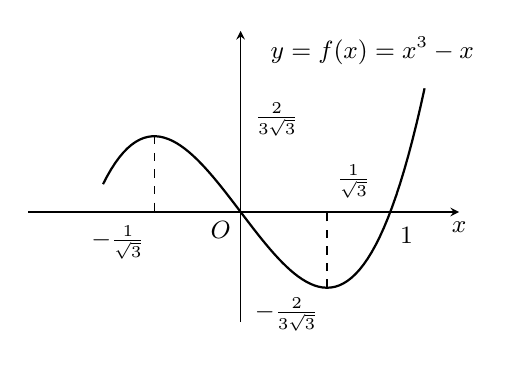
\begin{tikzpicture}[>=stealth,font=\small,x=1.9cm,y=2.5cm,
  baseline=(current bounding box.north)]
  \draw[->] (-1.42,0) -- (1.46,0) node[below] {$x$};
  \draw[->] (0,-0.56) -- (0,0.92);
  \node[below left] at (0,0) {$O$};
  \draw[thick] plot[domain=-0.92:1.23,samples=80] (\x,{(\x)^3-(\x)});
  \draw[dashed] (-0.577,0.385) -- (-0.577,0);
  \draw[dashed] (0.577,-0.385) -- (0.577,0);
  \node[right] at (0.03,0.47) {$\frac{2}{3\sqrt{3}}$};
  \node[right] at (0.03,-0.52) {$-\frac{2}{3\sqrt{3}}$};
  \node[below left] at (-0.577,-0.02) {$-\frac{1}{\sqrt{3}}$};
  \node[above right] at (0.577,0.02) {$\frac{1}{\sqrt{3}}$};
  \node[below right] at (1.0,-0.03) {$1$};
  \node[above] at (0.88,0.70) {$y=f(x)=x^{3}-x$};
\end{tikzpicture}
\caption{}\label{fig:3.5.1}
\end{minipage}
\end{figure}

由上可见, $-\frac{1}{\sqrt{3}}$ 与 $\frac{1}{\sqrt{3}}$ 分别为 $f(x)$ 在 $(-\infty,+\infty)$ 上的极大值点与极小值点 (如图~\ref{fig:3.5.1} 所示).
\end{solution}

\begin{example}\label{ex:3.5.4}
设 $n\in\mathbb{N}$, 证明:
\[
\mathrm{e}^{x}>1+\frac{x}{1!}+\frac{x^{2}}{2!}+\cdots+\frac{x^{n}}{n!},\quad\forall x>0.
\]
\end{example}

\begin{proof}
(数学归纳法) 当 $n=1$ 时, 令 $\varphi(x)=\mathrm{e}^{x}-(1+x)$, $x\geqslant 0$, 则 $\varphi'(x)=\mathrm{e}^{x}-1>0$, $x>0$. 这表明 $\varphi$ 在 $[0,+\infty)$ 上是严格增的. 于是,
\[
\mathrm{e}^{x}-(1+x)=\varphi(x)>\varphi(0)=0,
\]
\[
\mathrm{e}^{x}>1+x,\ x>0.
\]
不等式成立.

假设 $n=k$ 时, 有
\[
\mathrm{e}^{x}>1+\frac{x}{1!}+\frac{x^{2}}{2!}+\cdots+\frac{x^{k}}{k!},\quad x>0,
\]
则当 $n=k+1$ 时, 令
\[
\psi(x)=\mathrm{e}^{x}-\Big[1+\frac{x}{1!}+\frac{x^{2}}{2!}+\cdots+\frac{x^{k+1}}{(k+1)!}\Big],\quad x\geqslant 0.
\]
依归纳假设,
\[
\psi'(x)=\mathrm{e}^{x}-\Big(1+\frac{x}{1!}+\cdots+\frac{x^{k}}{k!}\Big)>0,\quad x>0.
\]
这表明 $\psi$ 在 $[0,+\infty)$ 上是严格增的. 于是,
\[
\psi(x)>\psi(0)=0,
\]
即
\[
\mathrm{e}^{x}>1+\frac{x}{1!}+\frac{x^{2}}{2!}+\cdots+\frac{x^{k}}{k!},\quad x>0.
\]
\end{proof}

\begin{example}\label{ex:3.5.5}
证明: $\frac{2}{\pi}\leqslant\frac{\sin x}{x}<1$, $x\in\left(0,\frac{\pi}{2}\right]$.
\end{example}

\begin{proof}
令 $f(x)=\frac{\sin x}{x}$, 则 $f'(x)=\frac{x\cos x-\sin x}{x^{2}}=\cos x\cdot\frac{x-\tan x}{x}<0$, $x\in\left(0,\frac{\pi}{2}\right)$, 从而 $f(x)$ 在 $\left(0,\frac{\pi}{2}\right]$ 上严格减. 又因为 $\lim\limits_{x\to 0}\frac{\sin x}{x}=1$, 所以
\[
\frac{2}{\pi}=\frac{\sin\frac{\pi}{2}}{\frac{\pi}{2}}\leqslant\frac{\sin x}{x}<1,\quad x\in\left(0,\frac{\pi}{2}\right].
\]
\end{proof}

\begin{example}\label{ex:3.5.6}
设 $f$ 在 $(a,+\infty)$ 上有有界的导函数. 证明: 存在常数 $C$ 与 $x_{0}$, 当 $x\geqslant x_{0}$ 时, $f(x)<Cx$.
\end{example}

\begin{proof}
设 $|f'(x)|\leqslant M$, $\forall x\in(a,+\infty)$. 取定 $x_{0}>0$, 再取 $C>\max\left\{M,\frac{f(x_{0})}{x_{0}}\right\}$. 令 $F(x)=f(x)-Cx$, 则
\[
F'(x)=f'(x)-C<0,
\]
根据定理~\ref{thm:3.5.1} 知, $F(x)$ 在 $(a,+\infty)$ 上严格减. 所以,
\[
f(x)-Cx=F(x)\leqslant F(x_{0})=f(x_{0})-Cx_{0}<0,\ \forall x\geqslant x_{0},
\]
即
\[
f(x)<Cx,\ \forall x\geqslant x_{0}.
\]
\end{proof}

\begin{example}\label{ex:3.5.7}
设 $f$ 在 $[a,+\infty)$ 上连续, 在 $(a,+\infty)$ 内可导, $f(a)<0$, 且当 $x>a$ 时, $f'(x)>k>0$. 证明: $f$ 有惟一的零点.
\end{example}

\begin{proof}
由 $f(a)<0$ 与 $k>0$ 知, $a-\frac{f(a)}{k}>a$. 在 $\left[a,a-\frac{f(a)}{k}\right]$ 上应用 Lagrange 中值定理, $\exists\xi\in\left(a,a-\frac{f(a)}{k}\right)$, s.t.
\[
\begin{aligned}
f\Big(a-\frac{f(a)}{k}\Big)-f(a)&=f'(\xi)\Big[\Big(a-\frac{f(a)}{k}\Big)-a\Big]\\
&=f'(\xi)\cdot\frac{-f(a)}{k}>k\cdot\frac{-f(a)}{k}\\
&=-f(a).
\end{aligned}
\]
因此得到 $f\left(a-\frac{f(a)}{k}\right)>0$. 根据零值定理可知, $\exists c\in\left(a,a-\frac{f(a)}{k}\right)$, s.t. $f(c)=0$.

另一方面, 由题设知, 当 $x>a$ 时, $f'(x)>k>0$, 因此, $f$ 在 $[a,+\infty)$ 上严格增, 从而 $f(x)=0$ 至多只有一个零点.

综上所述可推得 $f$ 有惟一的零点.
\end{proof}

\begin{example}\label{ex:3.5.8}
当 $x>0$ 时, 证明:
\[
\begin{aligned}
x-\frac{x^{3}}{3!}+\frac{x^{5}}{5!}-\cdots-\frac{x^{4k+3}}{(4k+3)!}&<\sin x\\
<x-\frac{x^{3}}{3!}+\frac{x^{5}}{5!}-\cdots-\frac{x^{4k-1}}{(4k-1)!}&+\frac{x^{4k+1}}{(4k+1)!},\\
1-\frac{x^{2}}{2!}+\frac{x^{4}}{4!}-\cdots-\frac{x^{4k+2}}{(4k+2)!}&<\cos x\\
<1-\frac{x^{2}}{2!}+\frac{x^{4}}{4!}-\cdots-\frac{x^{4k+2}}{(4k+2)!}&+\frac{x^{4k+4}}{(4k+4)!}.
\end{aligned}
\]
\end{example}

\begin{proof}
(1) 令 $F_{0}(x)=x-\sin x$, 则 $F'_{0}(x)=1-\cos x\geqslant 0$, 又 $\{x\in(0,+\infty)\mid F'(x)=1-\cos x=0\}=\{2k\pi\mid k\in\mathbb{N}\}$ 不构成区间, 根据定理~\ref{thm:3.5.3} 知, $F_{0}$ 在 $[0,+\infty)$ 上严格增. 于是,
\[
x-\sin x=F_{0}(x)>F(0)=0,
\]
即
\[
\sin x<x,\quad\forall x>0.
\]

(2) 令 $G_{0}(x)=\cos x-1+\frac{x^{2}}{2}$, 则由(1)知,
\[
G'_{0}(x)=-\sin x+x=x-\sin x>0,\quad\forall x>0,
\]
所以, $G_{0}(x)$ 在 $[0,+\infty)$ 上严格增. 于是,
\[
\cos x-1+\frac{x^{2}}{2}=G(x)>G(0)=0,
\]
即
\[
\cos x>1-\frac{x^{2}}{2},\quad\forall x>0.
\]

(3) 令 $H_{0}(x)=\sin x-x+\frac{x^{3}}{3!}$, 则由(2)知,
\[
H'_{0}(x)=\cos x-1+\frac{x^{2}}{2}>0,\quad\forall x>0,
\]
所以, $H_{0}(x)$ 在 $[0,+\infty)$ 上严格增. 于是,
\[
\sin x-x+\frac{x^{3}}{3!}=H(x)>H(0)=0,
\]
即
\[
\sin x>x-\frac{x^{3}}{3!},\quad\forall x>0.
\]

(4) 令 $Q_{0}(x)=1-\frac{x^{2}}{2!}+\frac{x^{4}}{4!}-\cos x$, 则由(3)知,
\[
Q'_{0}(x)=\sin x-x+\frac{x^{3}}{3!}>0,\quad\forall x>0,
\]
所以, $Q_{0}(x)$ 在 $[0,+\infty)$ 上严格增. 于是,
\[
1-\frac{x^{2}}{2!}+\frac{x^{4}}{4!}-\cos x=Q(x)>Q(0)=0,
\]
即
\[
\cos x<1-\frac{x^{2}}{2!}+\frac{x^{4}}{4!},\quad\forall x>0.
\]

余下请读者仿照以上(1)～(4)依次构造函数 $F_{l}(x)$, $G_{l}(x)$, $H_{l}(x)$, $Q_{l}(x)$, $l=1,2,\cdots$, 并应用归纳法完成不等式的全部证明.
\end{proof}

\begin{remark}\label{rem:3.5.1}
例~\ref{ex:3.5.4}、例~\ref{ex:3.5.5}、例~\ref{ex:3.5.8} 中各函数不等式的证法有一个共同之点, 就是先将不等式两边的函数移到一边去, 并构造一个新函数, 再应用导数证明新函数的单调性, 然后, 证明新函数大于零或小于零. 最终将移过来的函数移回去便得要证的不等式.
\end{remark}

Fermat 定理指出: 如果函数 $f$ 在 $x_{0}$ 达极值且可导, 则 $x_{0}$ 必为 $f$ 的驻点. 因此, $x_{0}$ 为 $f$ 的驻点是 $f$ 在 $x_{0}$ 可导下达到极值的必要条件, 但它不是充分条件. $y=f(x)=x^{3}$, $x_{0}=0$ 就是一个反例. 下面我们将给出两个达到极值的充分条件.

\begin{theorem}[极值的充分条件之一]\label{thm:3.5.4}
设 $f$ 在 $I$ 上有定义, $x_{0}\in\mathring{I}$ 为 $f$ 的连续点.

(1) 如果
\[
f'(x)\left\{
\begin{aligned}
&>0,\ x\in(x_{0}-\delta,x_{0}),\\
&<0,\ x\in(x_{0},x_{0}+\delta),
\end{aligned}
\right.
\]
则 $x_{0}$ 为 $f$ 的一个严格极大值点;

(2) $\exists\delta>0$, s.t.
\[
f'(x)\left\{
\begin{aligned}
&<0,\ x\in(x_{0}-\delta,x_{0}),\\
&>0,\ x\in(x_{0},x_{0}+\delta),
\end{aligned}
\right.
\]
则 $x_{0}$ 为 $f$ 的一个严格极小值点.
\end{theorem}

\begin{proof}
(1) 由定理~\ref{thm:3.5.1} 知, $f$ 在 $(x_{0}-\delta,x_{0}]$ 严格增, 所以 $f(x)<f(x_{0})$, $\forall x\in(x_{0}-\delta,x_{0})$; 再由定理~\ref{thm:3.5.1} 知, $f$ 在 $[x_{0},x_{0}+\delta)$ 上严格减, 所以 $f(x)<f(x_{0})$, $\forall x\in(x_{0},x_{0}+\delta)$. 这就证明了 $x_{0}$ 为 $f$ 的严格极大值点.

(2) 类似(1)证明, 或用 $-f$ 代替 $f$ 即可证得.
\end{proof}

读者自然会问: 如果 $x_{0}$ 为 $f$ 的驻点, 应再附加什么条件, $x_{0}$ 为 $f$ 的极值点, 是极大值点还是极小值点?

\begin{theorem}[极值的充分条件二]\label{thm:3.5.5}
设 $f$ 在 $I$ 上有定义, $x_{0}\in\mathring{I}$ 为 $f$ 的一个驻点, 即 $f'(x_{0})=0$. 进一步, 设 $f''(x_{0})$ 存在有限, 则:

(1) 当 $f''(x_{0})<0$ 时, $x_{0}$ 为 $f$ 的一个严格极大值点;

(2) 当 $f''(x_{0})>0$ 时, $x_{0}$ 为 $f$ 的一个严格极小值点.
\end{theorem}

\begin{proof}
(1) 因为
\[
\lim_{x\to x_{0}}\frac{f'(x)}{x-x_{0}}=\lim_{x\to x_{0}}\frac{f'(x)-f'(x_{0})}{x-x_{0}}=f''(x_{0})<0,
\]
所以, $\exists\delta>0$, s.t. 当 $0<|x-x_{0}|<\delta$ 时,
\[
\frac{f'(x)}{x-x_{0}}<0.
\]
由此可知,
\[
f'(x)\left\{
\begin{aligned}
&>0,\ x\in(x_{0}-\delta,x_{0}),\quad f\ \text{严格增},\\
&<0,\ x\in(x_{0},x_{0}+\delta),\quad f\ \text{严格减}.
\end{aligned}
\right.
\]
再由 $f$ 在 $x_{0}$ 可导, 从定理~\ref{thm:3.1.2} 知, $f$ 在 $x_{0}$ 连续. 根据定理~\ref{thm:3.5.4}(1) 推得, $x_{0}$ 为 $f$ 的极大值点.

(2) 类似(1)证明, 或用 $-f$ 代替 $f$ 即可证得.
\end{proof}

\begin{example}\label{ex:3.5.9}
上面两个定理只是判断严格极值的充分条件. 有这样的函数 $f$, 在它的严格极小值点 $x=0$ 的任何一侧都不具有单调的性质. 考察函数
\[
f(x)=\left\{
\begin{aligned}
&x\sin\frac{1}{x}+2|x|,\quad x\neq 0,\\
&0,\quad x=0.
\end{aligned}
\right.
\]
它是一个处处连续的偶函数. 因为 $\left|x\sin\frac{1}{x}\right|\leqslant|x|<2|x|$, $x\neq 0$, 所以 $f(x)>0=f(0)$.

从而 0 为 $f$ 的严格极小值(也是严格最小值). 但是, 当 $x>0$ 时,
\[
f'(x)=\sin\frac{1}{x}-\frac{1}{x}\cos\frac{1}{x}+2,
\]
所以, 对 $\forall n\in\mathbb{N}$, 有
\[
f'\left(\frac{1}{n\pi}\right)=0-n\pi\cdot(-1)^{n}+2=2+(-1)^{n+1}n\pi.
\]
当 $n$ 从 $1,2,3,\cdots$ 依次地跑过时, $f'\left(\frac{1}{n\pi}\right)$ 正负交替地改变符号, 因此 $\forall\delta>0$, 函数 $f$ 在区间 $(0,\delta)$ 上都不是单调的; 在 $(-\delta,0)$ 上也是这样.
\end{example}

\begin{corollary}\label{cor:3.5.1}
设 $f$ 在 $x_{0}$ 处 2 阶可导, $x_{0}$ 为 $f$ 的极大(小)值点, 则 $f''(x_{0})\leqslant 0(\geqslant 0)$.
\end{corollary}

\begin{proof}
(反证) 假设 $f''(x_{0})>0$, 由定理~\ref{thm:3.5.5}(2) 知, $x_{0}$ 为 $f$ 的严格极小值点, 又因为 $x_{0}$ 为 $f$ 的极大值点, 故 $\exists\delta>0$, 当 $0<|x-x_{0}|<\delta$ 时, 有
\[
f(x_{0})<f(x)\leqslant f(x_{0}),
\]
矛盾.

关于 $f''(x_{0})\geqslant 0$ 的情形可类似证明, 或用 $-f$ 代替 $f$ 即可证得.
\end{proof}

现在来讨论函数的最大值与最小值的问题, 这个问题有重大的理论价值与应用价值.

已经知道, 有界闭区间 $[a,b]$ 上的连续函数 $f$ 必达到它的最大值与最小值. 关于 $f$ 的最值有下面的定理.

\begin{theorem}\label{thm:3.5.6}
设 $f$ 为 $[a,b]$ 上的连续函数, 在 $(a,b)$ 内部, 除 $s_{1},s_{2},\cdots,s_{k}$ 外都可导, $t_{1},t_{2},\cdots,t_{l}$ 为 $f$ 的全部驻点, 则
\[
\begin{aligned}
\max_{a\leqslant x\leqslant b}f(x)&=\max\{f(a),f(s_{1}),\cdots,f(s_{k}),f(t_{1}),\cdots,f(t_{l}),f(b)\},\\
\min_{a\leqslant x\leqslant b}f(x)&=\min\{f(a),f(s_{1}),\cdots,f(s_{k}),f(t_{1}),\cdots,f(t_{l}),f(b)\}.
\end{aligned}
\]
\end{theorem}

\begin{proof}
因为 $f$ 为 $[a,b]$ 上的连续函数, 根据最值定理~\ref{thm:2.5.3} 知, $f$ 必达到它的最大值与最小值. 这最值点或者为 $a,b$; 或者为 $(a,b)$ 内部的不可导点; 或者为 $(a,b)$ 内部的极值点. 根据 Fermat 定理, 这种极值点必为 $f$ 的驻点. 综合上述得到
\[
\begin{aligned}
\max_{a\leqslant x\leqslant b}f(x)&=\max\{f(a),f(s_{1}),\cdots,f(s_{k}),f(t_{1}),\cdots,f(t_{l}),f(b)\},\\
\min_{a\leqslant x\leqslant b}f(x)&=\min\{f(a),f(s_{1}),\cdots,f(s_{k}),f(t_{1}),\cdots,f(t_{l}),f(b)\}.
\end{aligned}
\]
\end{proof}

\begin{example}\label{ex:3.5.10}
设 $f(x)=(x-1)(x-2)^{2}$. 求函数 $f$ 在 $\left[0,\frac{5}{2}\right]$ 上的最大值与最小值.
\end{example}

\begin{solution}
由 $f'(x)=(3x-4)(x-2)=0$, 得到 $f$ 的驻点为 $\frac{4}{3}$ 与 2. 于是, 根据定理~\ref{thm:3.5.6}, 有
\[
\begin{aligned}
\max_{0\leqslant x\leqslant\frac{5}{2}}f(x)&=\max_{0\leqslant x\leqslant\frac{5}{2}}\Big\{f(0),f\Big(\frac{4}{3}\Big),f(2),f\Big(\frac{5}{2}\Big)\Big\}\\
&=\max_{0\leqslant x\leqslant\frac{5}{2}}\Big\{-4,\frac{4}{27},0,\frac{3}{8}\Big\}=\frac{3}{8},
\end{aligned}
\]
\[
\begin{aligned}
\min_{0\leqslant x\leqslant\frac{5}{2}}f(x)&=\min_{0\leqslant x\leqslant\frac{5}{2}}\Big\{f(0),f\Big(\frac{4}{3}\Big),f(2),f\Big(\frac{5}{2}\Big)\Big\}\\
&=\min_{0\leqslant x\leqslant\frac{5}{2}}\Big\{-4,\frac{4}{27},0,\frac{3}{8}\Big\}=-4
\end{aligned}
\]
(如图~\ref{fig:3.5.2} 所示).
\end{solution}

\begin{figure}[htbp]
\centering
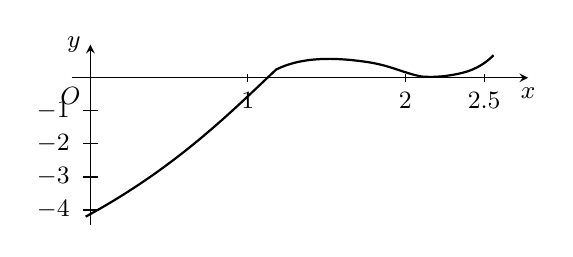
\begin{tikzpicture}[>=stealth,font=\small,x=2.0cm,y=0.42cm]
  \draw[->] (-0.12,0) -- (2.78,0) node[below] {$x$};
  \draw[->] (0,-4.45) -- (0,1.0) node[left] {$y$};
  \node[below left] at (0,0) {$O$};
  \draw[thick] (-0.03,-4.2)
    .. controls (0.55,-2.7) and (0.9,-1.0) .. (1.18,0.25)
    .. controls (1.32,0.58) and (1.5,0.64) .. (1.72,0.5)
    .. controls (1.9,0.4) and (1.98,0.15) .. (2.1,0.04)
    .. controls (2.2,-0.01) and (2.32,0.08) .. (2.4,0.2)
    .. controls (2.48,0.34) and (2.52,0.5) .. (2.56,0.68);
  \foreach \y/\l in {-1/-1,-2/-2,-3/-3,-4/-4}{
    \draw (0.05,\y) -- (-0.05,\y);
    \node[left] at (-0.07,\y) {$\l$};
  }
  \foreach \x/\l in {1/1,2/2,2.5/2.5}{
    \draw (\x,0.12) -- (\x,-0.12);
    \node[below] at (\x,-0.16) {$\l$};
  }
\end{tikzpicture}
\caption{}\label{fig:3.5.2}
\end{figure}

\begin{theorem}\label{thm:3.5.7}
设 $f$ 在区间 $I$ 上连续, 且只有惟一的极值点 $x_{0}$.

(1) 如果 $x_{0}$ 为 $f$ 的极大值点, 则 $x_{0}$ 为 $f$ 的惟一的最大值点;

(2) 如果 $x_{0}$ 为 $f$ 的极小值点, 则 $x_{0}$ 为 $f$ 的惟一的最小值点.
\end{theorem}

\begin{proof}
(1) (反证) 假设有 $x_{1}\neq x_{0}$, $x_{1}\in I$, 使 $f(x_{1})\geqslant f(x_{0})$, 不妨设 $x_{1}>x_{0}$. 由于 $f$ 在 $[x_{0},x_{1}]$ 上连续, 则它必有最小值. 因为 $x_{0}$ 为 $f$ 的极大值, 故 $\exists\delta>0$, 使得
\[
f(x)\leqslant f(x_{0}),\quad\forall x\in[x_{0},x_{0}+\delta),
\]
则必有 $x'\in(x_{0},x_{0}+\delta)$, 使 $f(x')<f(x_{0})$ (否则 $f(x)\equiv f(x_{0})$, $\forall x\in(x_{0},x_{0}+\delta)$, 从而 $(x_{0},x_{0}+\delta)$ 中任何点均为 $f$ 的极值点, 这与只有惟一的极值点 $x_{0}$ 相矛盾). 由以上讨论知, $x_{0}$ 与 $x_{1}$ 均不为 $f$ 在 $[x_{0},x_{1}]$ 中的最小值点. 其最小值点 $\xi\in(x_{0},x_{1})$, 当然 $\xi$ 为 $f$ 的极小值点, 这与 $x_{0}$ 为 $f$ 的惟一的极值点相矛盾.

(2) 可类似(1)证明, 或用 $-f$ 代替 $f$ 即可证得.
\end{proof}

\begin{example}\label{ex:3.5.11}
设 $m>0$, $n>0$, 则当 $0\leqslant x\leqslant a$ 时, 有
\[
x^{m}(a-x)^{n}\leqslant\frac{m^{m}n^{n}}{(m+n)^{m+n}}a^{m+n}.
\]
\end{example}

\begin{proof}
设 $f(x)=x^{m}(a-x)^{n}$, $0\leqslant x\leqslant a$, 则 $f(x)\geqslant 0$, 且
\[
\begin{aligned}
f'(x)&=mx^{m-1}(a-x)^{n}-nx^{m}(a-x)^{n-1}\\
&=x^{m-1}(a-x)^{n-1}[m(a-x)-nx]\\
&=x^{m-1}(a-x)^{n-1}[ma-(m+n)x]
\left\{
\begin{aligned}
&>0,\ 0\leqslant x<\frac{ma}{m+n},\quad f\ \text{单调增},\\
&=0,\ x=\frac{ma}{m+n},\quad f\ \text{取最大值},\\
&<0,\ \frac{ma}{m+n}<x\leqslant a,\quad f\ \text{单调减}.
\end{aligned}
\right.
\end{aligned}
\]
于是,
\[
\begin{aligned}
x^{m}(a-x)^{n}&=f(x)\leqslant f\Big(\frac{ma}{m+n}\Big)\\
&=\Big(\frac{ma}{m+n}\Big)^{m}\Big(a-\frac{ma}{m+n}\Big)^{n}\\
&=\frac{m^{m}}{(m+n)^{m}}\,\frac{n^{n}}{(m+n)^{n}}\,a^{m+n}\\
&=\frac{m^{n}n^{n}}{(m+n)^{m+n}}\,a^{m+n}.
\end{aligned}
\]
\end{proof}

\begin{example}\label{ex:3.5.12}
$1$, $\sqrt{2}=2^{\frac{1}{2}}$, $\sqrt[3]{3}=3^{\frac{1}{3}}$, $\cdots$, $\sqrt[n]{n}=n^{\frac{1}{n}}$, $\cdots$ 中哪一项最大.
\end{example}

\begin{solution}
令 $f(x)=x^{\frac{1}{x}}$, $x>0$, 则
\[
\begin{aligned}
f'(x)&=\big(\mathrm{e}^{\frac{1}{x}\ln x}\big)'=\mathrm{e}^{\frac{1}{x}\ln x}\Big(\frac{-1}{x^{2}}\ln x+\frac{1}{x}\cdot\frac{1}{x}\Big)\\
&=x^{\frac{1}{x}-2}(1-\ln x)
\left\{
\begin{aligned}
&>0,\quad 0<x<\mathrm{e},\ f\ \text{严格增},\\
&=0,\quad x=\mathrm{e},\ f\ \text{达最大值},\\
&<0,\quad x>\mathrm{e},\ f\ \text{严格减}.
\end{aligned}
\right.
\end{aligned}
\]
\[
\lim_{x\to 0^{+}}x^{\frac{1}{x}}=\lim_{x\to 0^{+}}\mathrm{e}^{\frac{1}{x}\ln x}=0,
\]
\[
\lim_{x\to+\infty}x^{\frac{1}{x}}=\mathrm{e}^{\lim\limits_{x\to+\infty}\frac{\ln x}{x}}=\mathrm{e}^{0}=1.
\]
由图~\ref{fig:3.5.3} 知, $\max\limits_{n\in\mathbb{N}}\sqrt[n]{n}=\max\limits_{n\in\mathbb{N}}n^{\frac{1}{n}}=\max\{\sqrt{2},\sqrt[3]{3}\}$, 所以 $\sqrt[3]{3}$ 为最大项.
\end{solution}

\begin{figure}[htbp]
\centering
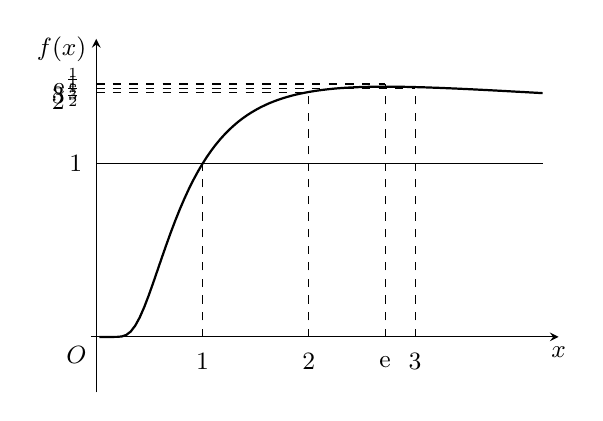
\begin{tikzpicture}[>=stealth,font=\small,x=1.35cm,y=2.2cm]
  \draw[->] (-0.05,0) -- (4.35,0) node[below] {$x$};
  \draw[->] (0,-0.32) -- (0,1.72);
  \node[left] at (0,1.66) {$f(x)$};
  \node[below left] at (0,0) {$O$};
  \draw (0,1) -- (4.2,1);
  \draw[thick] plot[domain=0.03:4.2,samples=100] (\x,{exp(ln(\x)/\x)});
  \draw[dashed] (1,0) -- (1,1);
  \draw[dashed] (2,0) -- (2,1.41);
  \draw[dashed] (2.71828,0) -- (2.71828,1.46);
  \draw[dashed] (3,0) -- (3,1.435);
  \draw[dashed] (0,1.41) -- (2,1.41);
  \draw[dashed] (0,1.46) -- (2.71828,1.46);
  \draw[dashed] (0,1.435) -- (3,1.435);
  \node[left] at (-0.04,1) {$1$};
  \node[left] at (-0.04,1.385) {$2^{\frac{1}{2}}$};
  \node[left] at (-0.04,1.425) {$3^{\frac{1}{3}}$};
  \node[left] at (-0.04,1.475) {$\mathrm{e}^{\frac{1}{\mathrm{e}}}$};
  \foreach \x/\l in {1/1,2/2,3/3}{
    \node[below] at (\x,-0.04) {$\l$};
  }
  \node[below] at (2.71828,-0.06) {$\mathrm{e}$};
\end{tikzpicture}
\caption{}\label{fig:3.5.3}
\end{figure}

\begin{example}\label{ex:3.5.13}
有长方形纸板, 长 8cm, 宽 5cm, 将四角各剪去大小相同的小正方形, 制成无盖纸盒. 问小正方形的边长为多少时, 盒子的容积最大.
\end{example}

\begin{solution}
设剪去的小正方形边长为 $x$, 则 $0<x<\frac{5}{2}$ (如图~\ref{fig:3.5.4} 所示). 纸盒容积为
\[
V=x(8-2x)(5-2x)=4x^{3}-26x^{2}+40x,
\]
\[
V'=12x^{2}-52x+40=4(3x-10)(x-1)
\]
所以, 在 $\left(0,\frac{5}{2}\right)$ 中 $V$ 的驻点为 1. 由
\[
V(0)=0,\ V(1)=18,\ V\Big(\frac{5}{2}\Big)=0
\]
知, 当 $x=1$(cm) 时, 容积 $V(1)=18$(cm$^{3}$) 为最大.
\end{solution}

\begin{figure}[htbp]
\centering
\begin{tikzpicture}[>=stealth,font=\small,scale=0.62]
  \draw[thick] (0,0) rectangle (8,5);
  \fill[pattern=north east lines] (0,0) rectangle (0.85,0.85);
  \fill[pattern=north east lines] (7.15,0) rectangle (8,0.85);
  \fill[pattern=north east lines] (0,4.15) rectangle (0.85,5);
  \fill[pattern=north east lines] (7.15,4.15) rectangle (8,5);
  \draw[decorate,decoration={brace,amplitude=4pt}] (0,5.15) -- (0.85,5.15);
  \node[above] at (0.42,5.2) {$x$};
  \draw[decorate,decoration={brace,amplitude=5pt}] (8.2,0) -- (8.2,5);
  \node[right,rotate=90] at (8.55,2.5) {$5\mathrm{cm}$};
  \draw[decorate,decoration={brace,amplitude=5pt,mirror}] (0,-0.22) -- (8,-0.22);
  \node[below] at (4,-0.34) {$8\mathrm{cm}$};
\end{tikzpicture}
\caption{}\label{fig:3.5.4}
\end{figure}

\begin{example}\label{ex:3.5.14}
设 $A$ 为铁路上一站, 从 $A$ 运原料到工厂 $C$, $C$ 距铁路的垂直距离为 $BC=20$km, $B$ 距 $A$ 的距离 $AB=150$km. 现欲在 $AB$ 之间找一点 $D$, 修公路与 $C$ 连接 (见图~\ref{fig:3.5.5}). 已知铁路运输与公路运输费用之比为 $3:5$. 问: $D$ 修在何处才能使运费最省.
\end{example}

\begin{solution}
设公路运费为 5, 则铁路运费为 3, 置 $D$ 于离 $B$ $x$ (单位: km) 处, 则运费
\[
y=f(x)=3(150-x)+5\sqrt{x^{2}+20^{2}},
\]
\[
0=f'(x)=-3+\frac{5x}{\sqrt{x^{2}+400}},
\]
\[
5x=3\sqrt{x^{2}+400},\ 25x^{2}=9x^{2}+3600,
\]
\[
16x^{2}=3600,\quad x=\pm 15.
\]
因此, 从
\[
f'(x)=-3+\frac{5x}{\sqrt{x^{2}+400}}
\left\{
\begin{aligned}
&<0,\quad x<15,\ f(x)\ \text{严格减},\\
&=0,\quad x=15,\ f(15)\ \text{为最小值},\\
&>0,\quad x>15,\ f(x)\ \text{严格增}
\end{aligned}
\right.
\]
可知 $f(x)$ 在 $x=15$ 达到最小值, 即 $D$ 应选在 $A$ 点与 $B$ 点之间距 $B$ 点 15km 处, 其运费最省 (如图~\ref{fig:3.5.5} 所示). 或者从
\[
f''(x)=\frac{1}{x^{2}+400}\left(\sqrt{x^{2}+400}-\frac{x^{2}}{\sqrt{x^{2}+400}}\right)=\frac{2000}{(x^{2}+400)^{3/2}}>0
\]
得到 $f'(x)$ 严格增, 再由 $f'(15)=0$ 推出
\[
f'(x)\left\{
\begin{aligned}
&<0,\quad x<15,\ f(x)\ \text{严格减},\\
&=0,\quad x=15,\ f(15)\ \text{为最小值},\\
&>0,\quad x>15,\ f(x)\ \text{严格增}.
\end{aligned}
\right.
\]
\end{solution}

\begin{figure}[htbp]
\centering
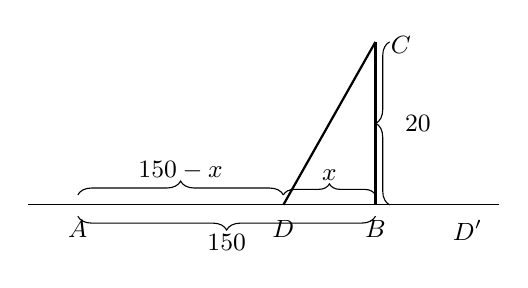
\begin{tikzpicture}[>=stealth,font=\small,scale=0.9]
  \draw (-0.35,0) -- (6.3,0);
  \draw[thick] (4.55,0) -- (4.55,2.3);
  \draw[thick] (3.25,0) -- (4.55,2.3);
  \draw[decorate,decoration={brace,amplitude=5pt}] (0.35,0.14) -- (3.25,0.14);
  \node[above] at (1.8,0.22) {$150-x$};
  \draw[decorate,decoration={brace,amplitude=4pt}] (3.25,0.14) -- (4.55,0.14);
  \node[above] at (3.9,0.2) {$x$};
  \draw[decorate,decoration={brace,amplitude=5pt}] (4.75,0) -- (4.75,2.3);
  \node[right] at (4.83,1.15) {$20$};
  \draw[decorate,decoration={brace,amplitude=5pt,mirror}] (0.35,-0.16) -- (4.55,-0.16);
  \node[below] at (2.45,-0.28) {$150$};
  \node[below] at (0.35,-0.08) {$A$};
  \node[below] at (3.25,-0.08) {$D$};
  \node[below] at (4.55,-0.08) {$B$};
  \node[below] at (5.85,-0.08) {$D'$};
  \node[right] at (4.63,2.25) {$C$};
\end{tikzpicture}
\caption{}\label{fig:3.5.5}
\end{figure}

\begin{example}\label{ex:3.5.15}
证明: 光线的入射角 $\theta_{\text{入}}$ 等于反射角 $\theta_{\text{反}}$.
\end{example}

\begin{proof}
光线服从``最短原理'': 光线从 $(0,a)$ 经 $x$ 轴上某点 $(x,0)$ 反射到 $(b,c)$ 点 (如图~\ref{fig:3.5.6} 所示). $x$ 在何处时, 所走路程 $AB+BC$ 最短.

设
\[
L(x)=AB+BC=\sqrt{a^{2}+x^{2}}+\sqrt{(b-x)^{2}+c^{2}}
\]
则
\[
L'(x)=\frac{x}{\sqrt{a^{2}+x^{2}}}-\frac{b-x}{\sqrt{(b-x)^{2}+c^{2}}},\quad 0\leqslant x\leqslant b,
\]
\[
\begin{aligned}
L''(x)&=\frac{1}{\sqrt{a^{2}+x^{2}}}-\frac{x^{2}}{\sqrt{(a^{2}+x^{2})^{3/2}}}+\frac{1}{\sqrt{(b-x)^{2}+c^{2}}}\\
&\quad-\frac{(b-x)^{2}}{\left[(b-x)^{2}+c^{2}\right]^{3/2}}\\
&=\frac{a^{2}+x^{2}-x^{2}}{(a^{2}+x^{2})^{3/2}}+\frac{(b-x)^{2}+c^{2}-(b-x)^{2}}{\left[(b-x)^{2}+c^{2}\right]^{3/2}}\\
&=\frac{a^{2}}{(a^{2}+x^{2})^{3/2}}+\frac{c^{2}}{\left[(b-x)^{2}+c^{2}\right]^{3/2}}>0.
\end{aligned}
\]
从而 $L'(x)$ 严格增, 且 $L(x)$ 在驻点 $\left(\frac{x}{\sqrt{a^{2}+x^{2}}}=\frac{b-x}{\sqrt{(b-x)^{2}+c^{2}}}\Longleftrightarrow\frac{a^{2}}{x^{2}}=\frac{c^{2}}{(b-x)^{2}}\Longleftrightarrow x=\frac{ab}{a+c}\right)$ 处达到最小值. 此时, $\triangle AOB\sim\triangle CDB$, 即 $\theta_{\text{入}}=\theta_{\text{反}}$.
\end{proof}

\begin{figure}[htbp]
\centering
\begin{tikzpicture}[>=stealth,font=\small,scale=1.0]
  \draw[->] (-0.1,0) -- (3.4,0) node[below] {$x$};
  \draw[->] (0,-0.12) -- (0,2.75);
  \node[left] at (0,2.68) {$y$};
  \node[below left] at (0,0) {$O$};
  \draw (2.95,0) -- (2.95,2.35);
  \draw[->] (0,2.0) -- (1.05,0);
  \draw[->] (1.05,0) -- (2.95,2.35);
  \draw[dashed] (1.05,0) -- (1.05,2.2);
  \draw (1.05,0.5) arc[start angle=90,end angle=117.7,radius=0.5];
  \draw (1.05,0.62) arc[start angle=50.3,end angle=90,radius=0.62];
  \node at (0.66,0.66) {$\theta_{\text{入}}$};
  \node at (1.5,0.86) {$\theta_{\text{反}}$};
  \node[above right] at (0,1.95) {$A(0,a)$};
  \node[below] at (1.05,-0.1) {$B(x,0)$};
  \node[below] at (2.95,-0.1) {$D(b,0)$};
  \node[right] at (2.99,2.35) {$C(b,c)$};
\end{tikzpicture}
\caption{}\label{fig:3.5.6}
\end{figure}

\begin{example}\label{ex:3.5.16}
炼油厂要修建容量为 $V_{0}$ 的贮油罐. 问: 此罐的底面直径与高之比为多少时, 用料量最省即表面积最小.
\end{example}

\begin{solution}
设油罐底面半径为 $r$, 高为 $h$, 则
\[
S=2\pi rh+2\pi r^{2}
\]
\[
V_{0}=\pi r^{2}h,\quad h=\frac{V_{0}}{\pi r^{2}},\quad r>0.
\]
于是,
\[
S=2\pi r\cdot\frac{V_{0}}{\pi r^{2}}+2\pi r^{2}=\frac{2V_{0}}{r}+2\pi r^{2},\quad r>0.
\]
\[
\begin{aligned}
S'&=-\frac{2V_{0}}{r^{2}}+4\pi r\\
&=\frac{2}{r^{2}}(2\pi r^{3}-V_{0})
\left\{
\begin{aligned}
&<0,\quad 0<r<\sqrt[3]{\frac{V_{0}}{2\pi}},\ S(r)\ \text{严格减},\\
&=0,\quad r=\sqrt[3]{\frac{V_{0}}{2\pi}},\ S\Big(\sqrt[3]{\frac{V_{0}}{2\pi}}\Big)\ \text{为最小值},\\
&>0,\quad r>\sqrt[3]{\frac{V_{0}}{2\pi}},\ S(r)\ \text{严格增},
\end{aligned}
\right.
\end{aligned}
\]
即当 $\frac{2r}{h}=\frac{2r}{\frac{V_{0}}{\pi r^{2}}}=\frac{2\pi r^{3}}{V_{0}}=\frac{2\pi\cdot\frac{V_{0}}{2\pi}}{V_{0}}=1$ 时, 表面积最省.
\end{solution}

\begin{exblock}{练习题 3.5}
  \item 确定下列函数的单调区间:
  \begin{enumerate}[label=(\arabic*)]
    \item $f(x)=3x-x^{2}$;
    \item $f(x)=2x^{2}-\ln x$;
    \item $f(x)=\sqrt{2x-x^{2}}$;
    \item $f(x)=\frac{x^{2}-1}{x}$;
    \item $f(x)=\arctan x-x$.
  \end{enumerate}

  \item 应用函数的单调性证明下列不等式:
  \begin{enumerate}[label=(\arabic*)]
    \item $\tan x>x-\frac{x^{3}}{3}$, $x\in\left(0,\frac{\pi}{3}\right)$;
    \item $\frac{2x}{\pi}<\sin x<x$, $x\in\left(0,\frac{\pi}{2}\right)$;
    \item $x-\frac{x^{2}}{2}<\ln(1+x)<x-\frac{x^{2}}{2(1+x)}$;
    \item $x(x-\arctan x)>0$, $x\neq 0$;
    \item $\ln(1+x)>\frac{\arctan x}{1+x}$, $x>0$.
  \end{enumerate}

  \item 设 $a,b>0$. 证明: 方程 $x^{3}+ax+b=0$ 不存在正根.

  \item 证明: $\frac{\tan x}{x}>\frac{x}{\sin x}$, $x\in\left(0,\frac{\pi}{2}\right)$.

  \item 设函数 $f$ 与 $g$ 在区间 $[a,+\infty)$ 上连续可导, 且当 $x>a$ 时, $|f'(x)|\leqslant g'(x)$. 证明: 当 $x\geqslant a$ 时,
  \[
  |f(x)-f(a)|\leqslant g(x)-g(a).
\]

  \item 设函数 $y=f(x)$ 在点 $x$ 处 3 阶可导, 且 $f'(x)\neq 0$. 证明: $f(x)$ 严格增或严格减, 从而存在反函数 $x=f^{-1}(y)$. 试用 $f'(x)$, $f''(x)$ 及 $f'''(x)$ 表示 $(f^{-1})''(y)$.

  \item 证明:
  (1) 方程 $x^{3}-3x+c=0$ ($c$ 为常数) 在区间 $[0,1]$ 内不可能有两个不同的实根.

  (2) 方程 $x^{n}+px+q=0$ ($n\in\mathbb{N}$, $p,q\in\mathbb{R}$) 当 $n$ 为偶数时至多有 2 个实根; 当 $n$ 为奇数时至多有 3 个实根.

  \item 设函数 $f$ 在 $[a,b]$ 上可导. 证明:
  (1) 若 $f'(x)\geqslant m$, 则 $f(x)\geqslant f(a)+m(x-a)$, $\forall x\in[a,b]$;

  (2) 若 $|f'(x)|\leqslant M$, 则 $|f(x)-f(a)|\leqslant M(x-a)$, $\forall x\in[a,b]$.

  \item 求下列函数的极值:
  \begin{enumerate}[label=(\arabic*)]
    \item $f(x)=2x^{3}-x^{4}$;
    \item $f(x)=\frac{2x}{1+x^{2}}$;
    \item $f(x)=\frac{(\ln x)^{2}}{x}$;
    \item $f(x)=\arctan x-\frac{1}{2}\ln(1+x^{2})$;
    \item $f(x)=|x(x^{2}-1)|$;
    \item $f(x)=(x-1)^{2}(x+1)^{3}$;
    \item $f(x)=\frac{x(x^{2}+1)}{x^{4}-x^{2}+1}$.
  \end{enumerate}

  \item 设
  \[
  f(x)=\left\{
  \begin{aligned}
  &x^{4}\sin^{2}\frac{1}{x},\quad x\neq 0,\\
  &0,\quad x=0.
  \end{aligned}
  \right.
\]
  (1) 证明: $x=0$ 为 $f$ 的极小值点, 也是最小值点;

  (2) 说明 $f$ 的极小值点 $x=0$ 处是否满足极值的充分条件一或充分条件二.

  \item 求下列函数在给定区间上的最大与最小值:
  \begin{enumerate}[label=(\arabic*)]
    \item $f(x)=x^{4}-2x^{2}+5$, $|x|\leqslant 2$;
    \item $f(x)=x^{5}-5x^{4}+5x^{3}+1$, $x\in[-1,2]$;
    \item $f(x)=x\ln x$, $x>0$;
    \item $f(x)=\sqrt{x}\ln x$, $x>0$;
    \item $f(x)=x^{2}-3x+2$, $x\in\mathbb{R}$;
    \item $f(x)=|x^{2}-3x+2|$, $|x|\leqslant 10$;
    \item $f(x)=2\tan x-\tan^{2}x$, $x\in\left[0,\frac{\pi}{2}\right)$;
    \item $f(x)=\arctan\frac{1-x}{1+x}$, $0\leqslant x\leqslant 1$.
  \end{enumerate}

  \item 设函数 $f$ 在点 $x_{0}$ 处有 $f'_{+}(x_{0})<0\,(>0)$, $f'_{-}(x_{0})>0\,(<0)$, 则 $x_{0}$ 为 $f$ 极大(小)值点.

  \item 证明: 当 $x>0$ 且 $x\neq 1$ 时, 有 $(1-x)\big(x^{2}\mathrm{e}^{\frac{1}{x}}-\mathrm{e}^{x}\big)>0$ (提示: 考察 $\varphi(x)=2\ln x+\frac{1}{x}-x$).

  \item 求一正数 $x$, 使它与其倒数之和 $f(x)=x+\frac{1}{x}$ 最小.

  \item 证明: (1) 周长为 $l$ 的矩形中, 以正方形所围面积最大; (2) 面积为定值 $S$ 的矩形中, 以正方形的边长为最小.

  \item 设用某仪器进行测量时, 读得 $n$ 次实验数据为 $a_{1},a_{2},\cdots,a_{n}$. 问以怎样的数值 $x$ 表达所要测量的真值, 才能使它与这 $n$ 个数之差的平方和为最小 (提示: 即证 $f(x)=\sum\limits_{i=1}^{n}(x-a_{i})^{2}$ 的最小值为 $\bar{x}=\frac{a_{1}+a_{2}+\cdots+a_{n}}{n}$).

  \item 内接于椭圆 $\frac{x^{2}}{a^{2}}+\frac{y^{2}}{b^{2}}=1$, 边平行于坐标轴的矩形, 何时面积最大.

  \item 从半径为 $R$ 的圆纸片上剪去一个扇形, 做成一个圆锥形的漏斗. 如何选取扇形的顶角, 可使漏斗的容积最大.

  \item 设 $0<a<b\leqslant 2a$, 在区间 $[a,b]$ 上讨论双曲线 $xy=1$. 在该曲线每一点上作切线, 它与横轴及两平行直线 $x=a$, $x=b$ 围成一个梯形. 问这切线位于何处, 才能使梯形有最大面积.

  \item 在抛物线 $y^{2}=2px$ 上哪一点的法线被抛物线所截之线段为最短.

  \item 有一个无盖的圆柱形容器, 当给定体积为 $V_{0}$ 时, 要使容器的表面积为最小, 问底的半径与容器高的比例为多大.

  \item 要将货物从运河边上 $A$ 城运往与运河相距 $a$ (单位: km) 的 $B$ 城, 轮船运费的单价是 $\alpha$ 元/km, 火车运费的单价是 $\beta$ 元/km ($\beta>\alpha$). 试求运河边上的一点 $M$, 修建铁路 $MB$, 使总运费最省.

  \item 重量为 $W$ 的物体放在一粗糙的平面上, 施加一力克服摩擦, 使之在平面上滑动, 其摩擦系数为 $\mu$, 问该力应与水平成何角度, 方可使用力最小?

  \item 设 $f(x)=a\ln x+bx^{2}+x$ 在 $x_{1}=1$, $x_{2}=2$ 处都取得极值, 试求 $a$ 与 $b$; 并问此时 $f$ 在 $x_{1}$ 与 $x_{2}$ 是取得极大值还是极小值.

  \item 证明: 定圆内接正 $n$ 边形面积随 $n$ 的增加而增加.

  \item 讨论函数
  \[
  f(x)=\left\{
  \begin{aligned}
  &\frac{x}{2}+x^{2}\sin\frac{1}{x},\quad x\neq 0,\\
  &0,\quad x=0.
  \end{aligned}
  \right.
\]
  (1) 在 $x=0$ 点是否可导.

  (2) 是否存在 $x=0$ 的一个开邻域, 使 $f$ 在该开邻域内单调.

  \item 设 $k>0$. 试问: $k$ 为何值时, 方程 $\arctan x-kx=0$ 有正实根.
\end{exblock}

\begin{exblock}{思考题 3.5}
  \item 设 $0<b<a$. 证明:
  \[
  \frac{a-b}{\sqrt{1+a^{2}}\sqrt{1+b^{2}}}<\arctan a-\arctan b<a-b,\quad\text{其中 } 0<b<a.
\]

  \item 证明下列不等式:
  (1) 当 $0<x_{1}<x_{2}<\frac{\pi}{2}$ 时, 有
  \[
  \frac{\tan x_{2}}{\tan x_{1}}>\frac{x_{2}}{x_{1}};
\]

  (2) 当 $x,y>0$ 且 $\beta>\alpha>0$ 时, 有
  \[
  (x^{\alpha}+y^{\alpha})^{\frac{1}{\alpha}}>(x^{\beta}+y^{\beta})^{\frac{1}{\beta}};
\]

  (3) 设 $p\geqslant 2$, 当 $x\in[0,1]$ 时, 有
  \[
  \left(\frac{1+x}{2}\right)^{p}+\left(\frac{1-x}{2}\right)^{p}\leqslant\frac{1}{2}(1+x^{p}).
\]

  \item 设函数 $f$ 在区间 $[0,+\infty)$ 上可导, $f(0)=0$ 且 $f'$ 严格增. 证明: $\frac{f(x)}{x}$ 在 $(0,+\infty)$ 上也严格增.

  \item 设求出使得不等式 $a^{x}\geqslant x^{a}$ ($x>0$) 成立的一切正数 $a$ (提示: 考察函数 $f(x)=\frac{\ln x}{x}$).

  \item 设 $f$ 在 $[a,+\infty)$ 上 2 阶可导, 且 $f(a)>0$, $f'(a)<0$, 当 $x>a$ 时, $f''(x)\leqslant 0$. 证明: 方程 $f(x)=0$ 在 $(a,+\infty)$ 内有且仅有一根.
\end{exblock}

% ==================================================================
%  徐森林、薛春华《数学分析》（第一册）
%  \S3.6  应用导数研究函数之二: 凹凸性、图形
% ==================================================================
%  源：原书印刷页 221-241（PDF 物理页 227-247）
%  底本：PaddleOCR-VL-1.6 + 高清影印比对校订
%  规范：全西文半角标点；单一落盘出口 _texout.py
% ==================================================================
\section{应用导数研究函数之二: 凹凸性、图形}\label{sec:3.6}

继 3.5 节, 应用 Lagrange 中值定理来研究函数的凹凸性.

\begin{definition}\label{def:3.6.1}
设 $f$ 为区间 $I$ 上的函数. 如果 $\forall x_{1},x_{2}\in I$, $\forall \lambda\in (0,1)$, 总有
\[
f(\lambda x_{1}+(1-\lambda)x_{2})\leqslant \lambda f(x_{1})+(1-\lambda)f(x_{2}),
\]
则称 $f$ 在 $I$ 上为\textbf{凸函数}(或\textbf{下凸函数}).

如果上述不等式中“$\leqslant$”改为“$<$”, 则称 $f$ 在 $I$ 上为\textbf{严格凸函数}(或\textbf{严格下凸函数}).

如果 $\forall x_{1},x_{2}\in I$, $\forall \lambda\in (0,1)$, 总有
\[
f(\lambda x_{1}+(1-\lambda)x_{2})\geqslant \lambda f(x_{1})+(1-\lambda)f(x_{2}),
\]
则称 $f$ 在 $I$ 上为\textbf{凹函数}.

如果上述不等式中“$\geqslant$”改为“$>$”, 则称 $f$ 在 $I$ 上为\textbf{严格凹函数}.
\end{definition}

从几何上看, 凸(凹)函数 $y=f(x)$ ($x\in I$) 的图形上的任何不同的两点间的曲线段完全落在连接该两点的直线段(称为曲线过这两点的\textbf{弦})的下(上)方、严格凸(凹)函数 $y=f(x)$ ($x\in I$) 的图形上的任何不同的两点间的曲线段完全严格落在该两点的弦的下(上)方(如图~\ref{fig:3.6.1}、图~\ref{fig:3.6.2} 所示, 其中 $x=\lambda x_{1}+(1-\lambda)x_{2}$).

\begin{figure}[htbp]
\centering
\begin{minipage}[t]{0.49\textwidth}
\centering
\begin{tikzpicture}[scale=0.72, >=Stealth, font=\small, baseline=(current bounding box.north)]
  \draw[->] (-0.3,0) -- (4.2,0) node[below] {$x$};
  \draw[->] (0,-0.3) -- (0,3.6) node[left] {$y$};
  \node[below left] at (0,0) {$O$};
  
  \draw[very thick] (0.5,0.7) to[out=10, in=250] (3.8,3.3) node[right] {$y=f(x)$};
  
  \def\xone{0.8}
  \def\xtwo{3.4}
  \def\xmid{2.2}
  
  \coordinate (P1) at (\xone, 0.74);
  \coordinate (P2) at (\xtwo, 2.6);
  \path (P1) -- (P2) coordinate[pos=0.538] (S);
  \coordinate (C) at (\xmid, 1.25);
  
  \draw[thick] (P1) -- (P2);
  
  \draw[dashed] (\xone,0) node[below] {$x_1$} -- (P1) -- (0,0.74) node[left] {$f(x_1)$};
  \draw[dashed] (\xtwo,0) node[below] {$x_2$} -- (P2) -- (0,2.6) node[left] {$f(x_2)$};
  \draw[dashed] (\xmid,0) node[below] {$x$} -- (S) -- (0,{1.87}) node[above left=-2pt] {\scriptsize $\lambda f(x_1)+(1-\lambda)f(x_2)$};
  \draw[dashed] (C) -- (0,1.25) node[left] {$f(x)$};
  
  \fill (P1) circle (1.5pt);
  \fill (P2) circle (1.5pt);
  \fill (S) circle (1.5pt);
  \fill (C) circle (1.5pt);
\end{tikzpicture}
\caption{凸函数}\label{fig:3.6.1}
\end{minipage}
\hfill
\begin{minipage}[t]{0.49\textwidth}
\centering
\begin{tikzpicture}[scale=0.72, >=Stealth, font=\small, baseline=(current bounding box.north)]
  \draw[->] (-0.3,0) -- (4.2,0) node[below] {$x$};
  \draw[->] (0,-0.3) -- (0,3.6) node[left] {$y$};
  \node[below left] at (0,0) {$O$};
  
  \draw[very thick] (0.5,0.7) to[out=70, in=190] (3.8,3.1) node[right] {$y=f(x)$};
  
  \def\xone{0.8}
  \def\xtwo{3.4}
  \def\xmid{2.2}
  
  \coordinate (P1) at (\xone, 1.35);
  \coordinate (P2) at (\xtwo, 2.95);
  \path (P1) -- (P2) coordinate[pos=0.538] (S);
  \coordinate (C) at (\xmid, 2.75);
  
  \draw[thick] (P1) -- (P2);
  
  \draw[dashed] (\xone,0) node[below] {$x_1$} -- (P1) -- (0,1.35) node[left] {$f(x_1)$};
  \draw[dashed] (\xtwo,0) node[below] {$x_2$} -- (P2) -- (0,2.95) node[left] {$f(x_2)$};
  \draw[dashed] (\xmid,0) node[below] {$x$} -- (C) -- (0,2.75) node[left] {$f(x)$};
  \draw[dashed] (S) -- (0,{2.21}) node[above left=-2pt] {\scriptsize $\lambda f(x_1)+(1-\lambda)f(x_2)$};
  
  \fill (P1) circle (1.5pt);
  \fill (P2) circle (1.5pt);
  \fill (S) circle (1.5pt);
  \fill (C) circle (1.5pt);
\end{tikzpicture}
\caption{凹函数}\label{fig:3.6.2}
\end{minipage}
\end{figure}

显然, $f$ 在区间 $I$ 上为(严格)凸(凹)函数 $\Longleftrightarrow -f$ 在区间 $I$ 上为(严格)凹(凸)函数. 因此, 凡对(严格)凸函数成立的命题, (严格)凹函数也成立相应的命题. 这可以类似(严格)凸函数的证明, 或者用 $-f$ 代替 $f$ 并应用(严格)凸函数的结论推得. 因此, 今后只须讨论(严格)凸函数的性质即可.

\begin{theorem}\label{thm:3.6.1}
$f$ 在区间 $I$ 中为凸函数 $\Longleftrightarrow \forall x_{1},x_{2},x_{3}\in I$, $x_{1}<x_{2}<x_{3}$, 下面不等式
\[
\frac{f(x_{2})-f(x_{1})}{x_{2}-x_{1}}\leqslant\frac{f(x_{3})-f(x_{1})}{x_{3}-x_{1}}\leqslant\frac{f(x_{3})-f(x_{2})}{x_{3}-x_{2}}
\]
中任何两个组成的不等式成立(如图~\ref{fig:3.6.3} 所示).
\end{theorem}

\begin{figure}[htbp]
\centering
\begin{tikzpicture}[scale=0.9, >=Stealth, font=\small]
  \draw[->] (-0.3,0) -- (5.0,0) node[below] {$x$};
  \draw[->] (0,-0.3) -- (0,4.2) node[left] {$y$};
  \node[below left] at (0,0) {$O$};
  
  \draw[very thick] (0.6,0.8) to[out=10, in=250] (4.2,3.8);
  
  \coordinate (P1) at (0.9, 0.95);
  \coordinate (P2) at (2.4, 1.6);
  \coordinate (P3) at (3.8, 3.4);
  
  \draw[thick] (P1) -- (P2) -- (P3) -- cycle;
  
  \draw[dashed] (P1) -- (0.9,0) node[below] {$x_1$};
  \draw[dashed] (P2) -- (2.4,0) node[below=1pt] {$x_2$};
  \node[below=14pt, align=center] at (2.4,0) {\scriptsize $x_2=\lambda x_1+(1-\lambda)x_3$\\[
1pt] \scriptsize $\lambda = \frac{x_3-x_2}{x_3-x_1}$};
  \draw[dashed] (P3) -- (3.8,0) node[below] {$x_3$};
  \fill (P1) circle (1.5pt) node[below left=-1pt] {$P_1(x_1,f(x_1))$};
  \fill (P2) circle (1.5pt) node[below right=-2pt] {$P_2(x_2,f(x_2))$};
  \fill (P3) circle (1.5pt) node[right=1pt] {$P_3(x_3,f(x_3))$};
\end{tikzpicture}
\caption{三条弦的斜率}\label{fig:3.6.3}
\end{figure}
\begin{proof}
(1) $f$ 在区间 $I$ 上为凸函数
\begin{align*}
&\Longleftrightarrow f(x_{2})=f\left(\frac{x_{3}-x_{2}}{x_{3}-x_{1}}x_{1}+\frac{x_{2}-x_{1}}{x_{3}-x_{1}}x_{3}\right)\\
&\quad\leqslant \frac{x_{3}-x_{2}}{x_{3}-x_{1}}f(x_{1})+\frac{x_{2}-x_{1}}{x_{3}-x_{1}}f(x_{3})\\
&\Longleftrightarrow f(x_{3})-f(x_{2})\geqslant \frac{x_{3}-x_{1}-x_{2}+x_{1}}{x_{3}-x_{1}}f(x_{3})-\frac{x_{3}-x_{2}}{x_{3}-x_{1}}f(x_{1})\\
&\quad=\frac{x_{3}-x_{2}}{x_{3}-x_{1}}f(x_{3})-\frac{x_{3}-x_{2}}{x_{3}-x_{1}}f(x_{1})\\
&\quad=\frac{x_{3}-x_{2}}{x_{3}-x_{1}}[f(x_{3})-f(x_{1})]\\
&\Longleftrightarrow \frac{f(x_{3})-f(x_{1})}{x_{3}-x_{1}}\leqslant \frac{f(x_{3})-f(x_{2})}{x_{3}-x_{2}}.
\end{align*}
(2) $f$ 在区间 $I$ 上为凸函数
\begin{align*}
&\Longleftrightarrow f(x_{2})-f(x_{1})\leqslant \frac{x_{3}-x_{2}-x_{3}+x_{1}}{x_{3}-x_{1}}f(x_{1})+\frac{x_{2}-x_{1}}{x_{3}-x_{1}}f(x_{3})\\
&\quad=-\frac{x_{2}-x_{1}}{x_{3}-x_{1}}f(x_{1})+\frac{x_{2}-x_{1}}{x_{3}-x_{1}}f(x_{3})\\
&\quad=\frac{x_{2}-x_{1}}{x_{3}-x_{1}}[f(x_{3})-f(x_{1})]\\
&\Longleftrightarrow \frac{f(x_{2})-f(x_{1})}{x_{2}-x_{1}}\leqslant \frac{f(x_{3})-f(x_{1})}{x_{3}-x_{1}}.
\end{align*}
(3) $f$ 在区间 $I$ 上为凸函数
\begin{align*}
&\Longleftrightarrow (x_{3}-x_{1})f(x_{2})\leqslant (x_{3}-x_{2})f(x_{1})+(x_{2}-x_{1})f(x_{3})\\
&\Longleftrightarrow -(x_{3}-x_{2})f(x_{1})\leqslant (x_{2}-x_{1})f(x_{3})-(x_{3}-x_{2}+x_{2}-x_{1})f(x_{2})\\
&\Longleftrightarrow (x_{3}-x_{2})[f(x_{2})-f(x_{1})]\leqslant (x_{2}-x_{1})[f(x_{3})-f(x_{2})]\\
&\Longleftrightarrow \frac{f(x_{2})-f(x_{1})}{x_{2}-x_{1}}\leqslant \frac{f(x_{3})-f(x_{2})}{x_{3}-x_{2}}.
\end{align*}
\end{proof}
观察一下定理~\ref{thm:3.6.1} 的几何意义是有帮助的. 在图~\ref{fig:3.6.3} 中, 画出了 $y=f(x)$ 的三条弦 $P_{1}P_{2},P_{2}P_{3},P_{1}P_{3}$, 其中 $P_{i}=(x_{i},f(x_{i}))$, $i=1,2,3$. 这三条弦组成了一个三角形. 定理~\ref{thm:3.6.1} 中不等式的几何表示是
\[
\overline{P_{1}P_{2}}\ \text{的斜率}\leqslant \overline{P_{1}P_{3}}\ \text{的斜率}\leqslant \overline{P_{2}P_{3}}\ \text{的斜率}.
\]
这正表示曲线 $y=f(x)$ 的下凸状态, 几何表示便于定理~\ref{thm:3.6.1} 中不等式的记忆.

关于凸函数, 有重要的 Jensen(詹森)不等式.

\begin{theorem}[Jensen 不等式]\label{thm:3.6.2}
$f$ 在区间 $I$ 上为凸函数 $\Longleftrightarrow \forall x_{i}\in I$, $\forall \lambda_{i}>0$ ($i=1,2,\cdots,n$), $\sum_{i=1}^{n}\lambda_{i}=1$, 有
\[
f\left(\sum_{i=1}^{n}\lambda_{i}x_{i}\right)\leqslant \sum_{i=1}^{n}\lambda_{i}f(x_{i}).
\]
如果 $f$ 在区间 $I$ 上为严格凸函数, 则当上述 $x_{1},x_{2},\cdots,x_{n}\in I$ 不全相等时, 有
\[
f\left(\sum_{i=1}^{n}\lambda_{i}x_{i}\right)< \sum_{i=1}^{n}\lambda_{i}f(x_{i}).
\]
\end{theorem}

\begin{proof}
($\Longrightarrow$) 设 $f$ 在区间 $I$ 上为凸函数.

(归纳法) 当 $n=1$ 时, $\lambda_{1}=1$, $f\left(\sum_{i=1}^{1}\lambda_{i}x_{i}\right)=f(\lambda_{1}x_{1})=f(x_{1})=\sum_{i=1}^{1}\lambda_{i}f(x_{i})$;

当 $n=2$ 时, $\lambda_{1}=\lambda$, $\lambda_{2}=1-\lambda$,
\[
f\left(\sum_{i=1}^{2}\lambda_{i}x_{i}\right)=f(\lambda x_{1}+(1-\lambda)x_{2})\leqslant \lambda f(x_{1})+(1-\lambda)f(x_{2})=\sum_{i=1}^{2}\lambda_{i}f(x_{i});
\]
假设 $n=k$ 时, $\forall x_{i}\in I$, $\forall \lambda_{i}>0$ ($i=1,2,\cdots,k$), $\sum_{i=1}^{k}\lambda_{i}=1$, 有
\[
f\left(\sum_{i=1}^{k}\lambda_{i}x_{i}\right)\leqslant \sum_{i=1}^{k}\lambda_{i}f(x_{i}),
\]
则当 $n=k+1$ 时, $\forall x_{i}\in I$, $\forall \lambda_{i}>0$ ($i=1,2,\cdots,k+1$), $\sum_{i=1}^{k+1}\lambda_{i}=1$. 令 $\mu_{i}=\frac{\lambda_{i}}{1-\lambda_{k+1}}$, $i=1,2,\cdots,k$, 便有 $\mu_{i}>0$ 且 $\sum_{i=1}^{k}\mu_{i}=\sum_{i=1}^{k}\frac{\lambda_{i}}{1-\lambda_{k+1}}=\frac{1-\lambda_{k+1}}{1-\lambda_{k+1}}=1$. 于是,
\begin{align*}
f\left(\sum_{i=1}^{k+1}\lambda_{i}x_{i}\right)&=f\left((1-\lambda_{k+1})\sum_{i=1}^{k}\frac{\lambda_{i}}{1-\lambda_{k+1}}x_{i}+\lambda_{k+1}x_{k+1}\right)\\
&\leqslant (1-\lambda_{k+1})f\left(\sum_{i=1}^{k}\frac{\lambda_{i}}{1-\lambda_{k+1}}x_{i}\right)+\lambda_{k+1}f(x_{k+1}).
\end{align*}
归纳可得
\begin{align*}
f\left(\sum_{i=1}^{k+1}\lambda_{i}x_{i}\right)&\leqslant (1-\lambda_{k+1})\sum_{i=1}^{k}\frac{\lambda_{i}}{1-\lambda_{k+1}}f(x_{i})+\lambda_{k+1}f(x_{k+1})\\
&=\sum_{i=1}^{k+1}\lambda_{i}f(x_{i}).
\end{align*}

($\Longleftarrow$) 如果右边条件成立, 特别当 $n=2$ 时, $\lambda=\lambda_{1}$, $1-\lambda=1-\lambda_{1}=\lambda_{2}$, 故有
\[
f(\lambda x_{1}+(1-\lambda)x_{2})=f(\lambda_{1}x_{1}+\lambda_{2}x_{2})\leqslant \lambda_{1}f(x_{1})+\lambda_{2}f(x_{2})=\lambda f(x_{1})+(1-\lambda)f(x_{2}).
\]
这就证明了 $f$ 在区间 $I$ 上为凸函数.

关于严格凸函数情形, 当 $x_{1},x_{2},\cdots,x_{n}$ 不全相等时, 我们重新审查归纳证明. 当 $n=2$ 时, $x_{1},x_{2}$ 不全相等就是 $x_{1}\neq x_{2}$, 按定义, 严格的不等号成立. 假设 $n=k$ 时, 严格不等号成立. 再设 $x_{1},x_{2},\cdots,x_{k+1}$ 不全相等, 如果其中 $x_{1},x_{2},\cdots,x_{k}$ 不全相等, 则上述归纳法中最后的那个不等号应当是严格的; 如果 $x_{1}=\cdots=x_{k}\neq x_{k+1}$, 则 $\sum_{i=1}^{k}\mu_{i}x_{i}=x_{1}\sum_{i=1}^{k}\mu_{i}=x_{1}\neq x_{k+1}$, 此时归纳过程的第 1 个不等号是严格的. 总之, 不等式
\[
f\left(\sum_{i=1}^{n}\lambda_{i}x_{i}\right)<\sum_{i=1}^{n}\lambda_{i}f(x_{i})
\]
对一切 $n\in\mathbb{N}$ 成立.
\end{proof}

\begin{theoremp}[Jensen 不等式]\label{thm:3.6.2p}
$f$ 在区间 $I$ 上为凸函数 $\Longleftrightarrow \forall x_{i}\in I$, $\forall \beta_{i}>0$ ($i=1,2,\cdots,n$), 有
\[
f\left(\frac{\displaystyle\sum_{i=1}^{n}\beta_{i}x_{i}}{\displaystyle\sum_{i=1}^{n}\beta_{i}}\right)\leqslant\frac{\displaystyle\sum_{i=1}^{n}\beta_{i}f(x_{i})}{\displaystyle\sum_{i=1}^{n}\beta_{i}}.
\]
如果 $f$ 是严格凸的, 则当上述 $x_{1},x_{2},\cdots,x_{n}\in I$ 不全相等时有
\[
f\left(\frac{\displaystyle\sum_{i=1}^{n}\beta_{i}x_{i}}{\displaystyle\sum_{i=1}^{n}\beta_{i}}\right)<\frac{\displaystyle\sum_{i=1}^{n}\beta_{i}f(x_{i})}{\displaystyle\sum_{i=1}^{n}\beta_{i}}.
\]
\end{theoremp}

在函数 $f$ 有导函数 $f'$ 的情况下, 判断 $f$ 的凸性将变得比较容易, 因为我们有下面定理.

\begin{theorem}\label{thm:3.6.3}
设 $f$ 在区间 $I$ 上可导, 则下面三个结论等价:
\begin{enumerate}[label=(\arabic*)]
  \item $f$ 在 $I$ 上为(严格)凸函数;
  \item $f'$ 在 $I$ 上为(严格)增函数;
  \item $\forall x_{0},x\in I$, $x\neq x_{0}$, 有
  \[
  f(x)\geqslant f(x_{0})+f'(x_{0})(x-x_{0})
\]
  (或 $f(x)>f(x_{0})+f'(x_{0})(x-x_{0})$), 即 $f$ 的图形(严格)在其任一点 $(x_{0},f(x_{0}))$ 的切线的上方.
\end{enumerate}
\end{theorem}

\begin{figure}[htbp]
\centering
\begin{tikzpicture}[scale=0.9, >=Stealth, font=\small]
  \draw[->] (-0.3,0) -- (4.8,0) node[below] {$x$};
  \draw[->] (0,-0.3) -- (0,4.2) node[left] {$y$};
  \node[below left] at (0,0) {$O$};
  
  \draw[very thick] (0.8,1.2) to[out=5, in=250] (3.8,3.6);
  
  \coordinate (P1) at (1.0, 1.25);
  \coordinate (P1h) at (1.6, 1.35);
  \coordinate (P2h) at (3.1, 2.55);
  \coordinate (P2) at (3.8, 3.6);
  
  \draw[thick] (P1) -- (P2);
  \draw[dashed] (P1) -- (P1h);
  \draw[dashed] (P2h) -- (P2);
  
  \draw[dashed] (P1) -- (1.0,0) node[below] {$x_1$};
  \draw[dashed] (P1h) -- (1.6,0) node[below] {$x_1+h$};
  \draw[dashed] (P2h) -- (3.1,0) node[below] {$x_2-h$};
  \draw[dashed] (P2) -- (3.8,0) node[below] {$x_2$};
  
  \fill (P1) circle (1.5pt) node[above left=-1pt] {$(x_1,f(x_1))$};
  \fill (P1h) circle (1.5pt) node[below right=-1pt] {$(x_1+h,f(x_1+h))$};
  \fill (P2h) circle (1.5pt) node[right=1pt] {$(x_2-h,f(x_2-h))$};
  \fill (P2) circle (1.5pt) node[right=1pt] {$(x_2,f(x_2))$};
\end{tikzpicture}
\caption{割线斜率的逼近}\label{fig:3.6.4}
\end{figure}

\begin{proof}
(1) $\Longrightarrow$ (2) 设 $f$ 在 $I$ 上为凸函数, 即 $\forall x_{1},x_{2}\in I$, $x_{1}<x_{2}$, 充分小的 $h>0$, 使得 $x_{1}<x_{1}+h<x_{2}-h<x_{2}$. 根据 $f$ 的凸性及定理~\ref{thm:3.6.1}, 有(如图~\ref{fig:3.6.4} 所示)
\[
\frac{f(x_{1}+h)-f(x_{1})}{h}\leqslant\frac{f(x_{2})-f(x_{1})}{x_{2}-x_{1}}\leqslant\frac{f(x_{2})-f(x_{2}-h)}{h}.
\]
因为 $f$ 可导, 令 $h\to 0^{+}$, 得到
\[
f'(x_{1})=f'_{+}(x_{1})\leqslant\frac{f(x_{2})-f(x_{1})}{x_{2}-x_{1}}\leqslant f'_{-}(x_{2})=f'(x_{2}),
\]
所以, $f'$ 在 $I$ 上为增函数.

在 $f$ 为严格凸函数的情形时, 我们取定一点 $x^{*}\in (x_{1},x_{2})$, 从而得出
\[
f'(x_{1})\leqslant\frac{f(x^{*})-f(x_{1})}{x^{*}-x_{1}}<\frac{f(x_{2})-f(x^{*})}{x_{2}-x^{*}}\leqslant f'(x_{2}).
\]
这就得出了严格不等式 $f'(x_{1})<f'(x_{2})$, 即 $f'$ 在 $I$ 上为严格增函数.

(1) $\Longleftarrow$ (2) 设 $f'$ 在 $I$ 上为增函数. 对任何 $x_{1}<x_{2}<x_{3}$, 由 Lagrange 中值定理知, 存在 $x_{1}<\xi_{1}<x_{2}<\xi_{2}<x_{3}$, 使得
\[
\frac{f(x_{2})-f(x_{1})}{x_{2}-x_{1}}=f'(\xi_{1})\leqslant f'(\xi_{2})=\frac{f(x_{3})-f(x_{2})}{x_{3}-x_{2}}.
\]
再根据定理~\ref{thm:3.6.1} 知, $f$ 在 $I$ 上为凸函数.

如果 $f'$ 在 $I$ 上为严格增函数, 则上述不等式为
\[
\frac{f(x_{2})-f(x_{1})}{x_{2}-x_{1}}=f'(\xi_{1})<f'(\xi_{2})=\frac{f(x_{3})-f(x_{2})}{x_{3}-x_{2}},
\]
再由定理~\ref{thm:3.6.1}, $f$ 在 $I$ 上为严格凸函数.

(2) $\Longrightarrow$ (3) 设 $f'$ 在 $I$ 为增函数. $\forall x_{0},x\in I$, 由 Lagrange 中值定理知, 存在介于 $x_{0}$ 与 $x$ 之间的 $\xi$, 使得
\begin{align*}
f(x)-[f(x_{0})+f'(x_{0})(x-x_{0})]&=[f(x)-f(x_{0})]-f'(x_{0})(x-x_{0})\\
&=f'(\xi)(x-x_{0})-f'(x_{0})(x-x_{0})\\
&=[f'(\xi)-f'(x_{0})](x-x_{0})\geqslant 0,
\end{align*}
即 $f(x)\geqslant f(x_{0})+f'(x_{0})(x-x_{0})$, 即 $f$ 的图形落在 $(x_{0},f(x_{0}))$ 的切线的上方.

如果 $f'$ 在 $I$ 为严格增函数, $\forall x_{0},x\in I$, $x\neq x_{0}$, 上述不等式为
\[
f(x)-[f(x_{0})+f'(x_{0})(x-x_{0})]=[f'(\xi)-f'(x_{0})](x-x_{0})>0,
\]
即 $f(x)>f(x_{0})+f'(x_{0})(x-x_{0})$, 即 $f$ 的图形严格落在 $(x_{0},f(x_{0}))$ 的切线的上方.

(1) $\Longleftarrow$ (3) $\forall x_{1},x_{2}\in I$, $x_{1}<x_{2}$, 令 $x_{3}=\lambda x_{1}+(1-\lambda)x_{2}$, $0<\lambda<1$. 由 (3) 并利用
\[
x_{1}-x_{3}=(1-\lambda)(x_{1}-x_{2}),\quad x_{2}-x_{3}=\lambda(x_{2}-x_{1})
\]
得到
\[
f(x_{1})\geqslant f(x_{3})+f'(x_{3})(x_{1}-x_{3})=f(x_{3})+(1-\lambda)(x_{1}-x_{2})f'(x_{3}),
\]
\[
f(x_{2})\geqslant f(x_{3})+f'(x_{3})(x_{2}-x_{3})=f(x_{3})+\lambda(x_{2}-x_{1})f'(x_{3}).
\]
于是,
\begin{align*}
\lambda f(x_{1})+(1-\lambda)f(x_{2})&\geqslant \lambda[f(x_{3})+(1-\lambda)(x_{1}-x_{2})f'(x_{3})]\\
&\quad +(1-\lambda)[f(x_{3})+\lambda(x_{2}-x_{1})f'(x_{3})]\\
&=f(x_{3})=f(\lambda x_{1}+(1-\lambda)x_{2}),
\end{align*}
即 $f$ 在 $I$ 上为凸函数.

如果 $f$ 的图形严格在曲线每一点 $(x_{0},f(x_{0}))$, $x_{0}\in I$ 的切线的上方, 则上述不等式中所有的“$\geqslant$”均为“$>$”. 于是,
\[
\lambda f(x_{1})+(1-\lambda)f(x_{2})>f(\lambda x_{1}+(1-\lambda)x_{2}),
\]
即 $f$ 在 $I$ 上为严格凸函数.

(2) $\Longleftarrow$ (3) 由 (3), $\forall x_{1},x_{2}\in I$, $x_{1}<x_{2}$, 有
\begin{align*}
f(x_{1})&\geqslant f(x_{2})+f'(x_{2})(x_{1}-x_{2}),\\
f(x_{2})&\geqslant f(x_{1})+f'(x_{1})(x_{2}-x_{1}),
\end{align*}
从而
\[
f'(x_{1})\leqslant\frac{f(x_{2})-f(x_{1})}{x_{2}-x_{1}}\leqslant f'(x_{2}),
\]
即 $f'$ 在 $I$ 上为单调增函数.

如果 $f$ 的图形严格在曲线每一点 $(x_{0},f(x_{0}))$, $x_{0}\in I$ 的切线的上方, 则上述“$\geqslant$”均为“$>$”. 于是,
\[
f'(x_{1})<\frac{f(x_{2})-f(x_{1})}{x_{2}-x_{1}}<f'(x_{2}),
\]
即 $f'$ 在 $I$ 上为严格增函数.
\end{proof}

当 $f$ 在 $\mathring{I}=(a,b)$ 内二阶可导时, 我们有下面应用起来更方便的定理.

\begin{theorem}\label{thm:3.6.4}
设 $f$ 在区间 $I$ 上二阶可导, 则 $f$ 在 $I$ 上为(严格)凸函数 $\Longleftrightarrow f''(x)\geqslant 0$, $\forall x\in I$ ($f''(x)\geqslant 0$, $\forall x\in\mathring{I}$, 且 $\{x\in I\mid f''(x)=0\}$ 不含非退化区间).
\end{theorem}

\begin{proof}
$f$ 在 $I$ 上为(严格)凸函数
\[
\xLongleftrightarrow{\text{定理~3.6.3}} f'\ \text{在}\ I\ \text{上为(严格)单调增函数}
\]
\[
\xLongleftrightarrow[\text{定理~3.5.3}]{\text{定理~3.5.2}} f''(x)\geqslant 0,\ \forall x\in I\ (f''(x)\geqslant 0,\ \forall x\in\mathring{I},\ \text{且}\ \{x\in I\mid f''(x)=0\}\ \text{不含非退化区间}). \qedhere
\]
\end{proof}

上面详细讨论了曲线 $y=f(x)$ 的凹凸性. 研究凹与凸交界的点是十分有意义的.

\begin{definition}\label{def:3.6.2}
设连续曲线 $y=f(x)$ 在点 $(x_{0},f(x_{0}))$ 的近旁的两侧分别是严格凸(凹)与严格凹(凸)的, 则称点 $(x_{0},f(x_{0}))$ 或 $x_{0}$ 为 $y=f(x)$ 的\textbf{拐点}(如图~\ref{fig:3.6.5}、图~\ref{fig:3.6.6} 所示).
\end{definition}

\begin{figure}[htbp]
\centering
\begin{minipage}[t]{0.49\textwidth}
\centering
\begin{tikzpicture}[scale=0.72, >=Stealth, font=\small, baseline=(current bounding box.north)]
  \draw[->] (-0.3,0) -- (4.2,0) node[below] {$x$};
  \draw[->] (0,-0.3) -- (0,3.2) node[left] {$y$};
  \node[below left] at (0,0) {$O$};
  
  \coordinate (X0) at (1.8, 1.8);
  
  \draw[very thick] (0.6, 1.3) to[out=-20, in=210] (X0) to[out=30, in=190] (3.0, 2.0);
  
  \draw[dashed] (1.8,0) node[below] {$x_0$} -- (1.8, 2.8);
  \draw[dashed] (0,1.8) node[left] {$f(x_0)$} -- (X0);
  
  \fill (X0) circle (1.5pt);
  \node[above=6pt] at (X0) {拐点};
  \node[above left] at (1.3, 1.5) {凸};
  \node[below right] at (2.2, 1.8) {凹};
\end{tikzpicture}
\caption{由凸变凹拐点}\label{fig:3.6.5}
\end{minipage}
\hfill
\begin{minipage}[t]{0.49\textwidth}
\centering
\begin{tikzpicture}[scale=0.72, >=Stealth, font=\small, baseline=(current bounding box.north)]
  \draw[->] (-0.3,0) -- (4.2,0) node[below] {$x$};
  \draw[->] (0,-0.3) -- (0,3.2) node[left] {$y$};
  \node[below left] at (0,0) {$O$};
  
  \coordinate (X0) at (2.0, 1.8);
  
  \draw[very thick] (0.8, 1.95) to[out=20, in=150] (X0) to[out=-30, in=200] (3.2, 1.55);
  
  \draw[dashed] (2.0,0) node[below] {$x_0$} -- (2.0, 2.8);
  \draw[dashed] (0,1.8) node[left] {$f(x_0)$} -- (X0);
  
  \fill (X0) circle (1.5pt);
  \node[above=6pt] at (X0) {拐点};
  \node[below left] at (1.6, 1.7) {凹};
  \node[above right] at (2.4, 1.7) {凸};
\end{tikzpicture}
\caption{由凹变凸拐点}\label{fig:3.6.6}
\end{minipage}
\end{figure}

由定义可见, 拐点正是严格凸(凹)与严格凹(凸)的分界点.

\begin{theorem}\label{thm:3.6.5}
设 $f$ 在 $x_{0}$ 处二阶可导, 并且 $x_{0}$ 为 $f$ 的拐点, 则 $f''(x_{0})=0$. 但反之不真.
\end{theorem}

\begin{proof}
因为 $f$ 在 $x_{0}$ 处 2 阶可导, 所以 $f$ 在 $x_{0}$ 近旁可导. 又因 $x_{0}$ 为 $f$ 的拐点, 故 $(x_{0},f(x_{0}))$ 为严格凸(凹)与严格凹(凸)的分界点. 根据定理~\ref{thm:3.6.3} 可知, $f'$ 以 $x_{0}$ 为严格增(减)与严格减(增)的分界点. 由此推得 $x_{0}$ 为 $f'$ 的极大(小)值点. 根据 Fermat 定理立即知 $f''(x_{0})=0$.

反过来, 考虑函数 $y=f(x)=x^{4}$, $f'(x)=4x^{3}$,
\[
y''(x)=f''(x)\left\{
\begin{aligned}
&>0, &&x<0, f\ \text{严格凸},\\
&=0, &&x=0, \text{非拐点},\\
&>0, &&x>0, f\ \text{严格凸},
\end{aligned}\right.
\]
$f''(0)=0$, 但 $(0,f(0))=(0,0)$ 不是拐点.
\end{proof}

\begin{theorem}\label{thm:3.6.6}
设连续曲线 $y=f(x)$ 在 $x_{0}$ 的某去心开邻域 $U^{\circ}(x_{0})$ 内 2 阶可导. 如果在 $U_{+}^{\circ}(x_{0})$ 与 $U_{-}^{\circ}(x_{0})$ 内 $f''$ 的符号相反, 则 $(x_{0},f(x_{0}))$ 为曲线 $y=f(x)$ 的拐点.
\end{theorem}

\begin{proof}
由于在 $U_{+}^{\circ}(x_{0})$ 与 $U_{-}^{\circ}(x_{0})$ 内 $f''$ 的符号相反, 故凹凸性也相反, 从而 $(x_{0},f(x_{0}))$ 为 $y=f(x)$ 的拐点.
\end{proof}

\begin{example}\label{ex:3.6.1}
研究下列函数的凹凸性与拐点:
\begin{enumerate}[label=(\arabic*)]
  \item $y=\arctan x$;
  \item $y=\sqrt[3]{x}=x^{\frac{1}{3}}$;
  \item $y=\sin x$.
\end{enumerate}
\end{example}

\begin{solution}
(1) 从
\[
y'=\frac{1}{1+x^{2}}\left\{
\begin{aligned}
&\text{严格增}, &&x<0, &&y\ \text{严格凸},\\
&\text{严格减}, &&x>0, &&y\ \text{严格凹}
\end{aligned}\right.
\]
知 $(0,0)$ 为 $y=\arctan x$ 的拐点(如图~\ref{fig:3.6.7} 所示).

\begin{figure}[htbp]
\centering
\begin{tikzpicture}[scale=0.9, >=Stealth, font=\small]
  \draw[->] (-2.8,0) -- (3.2,0) node[below] {$x$};
  \draw[->] (0,-2.0) -- (0,2.2) node[left] {$y$};
  \node[below right] at (0,0) {$O$};
  
  \draw[thick] (-2.8, 1.57) -- (3.0, 1.57);
  \draw[thick] (-2.8, -1.57) -- (3.0, -1.57);
  \node[above right] at (0, 1.57) {$\frac{\pi}{2}$};
  \node[below right] at (0, -1.57) {$-\frac{\pi}{2}$};
  
  \draw[very thick] plot[domain=-2.7:2.7, samples=60] (\x, {rad(atan(\x))});
  
  \node[above left] at (-1.2, -0.9) {凸};
  \node[below right] at (1.2, 0.9) {凹};
\end{tikzpicture}
\caption{$y=\arctan x$ 的图形}\label{fig:3.6.7}
\end{figure}

或者
\[
y''=\frac{-2x}{(1+x^{2})^{2}}\left\{
\begin{aligned}
&>0, &&x<0, y\ \text{严格凸},\\
&=0, &&x=0, \text{拐点},\\
&<0, &&x>0, y\ \text{严格凹}.
\end{aligned}\right.
\]

(2) 从
\[
y'=\frac{1}{3}x^{-\frac{2}{3}}\left\{
\begin{aligned}
&\text{严格增}, &&x<0, &&y\ \text{严格凸},\\
&\text{严格减}, &&x>0, &&y\ \text{严格凹}
\end{aligned}\right.
\]
知 $(0,0)$ 为 $y=\sqrt[3]{x}$ 的拐点. 注意, 在 $x=0$ 处,
\[
y'(0)=\lim_{x\to 0}\frac{\sqrt[3]{x}-0}{x-0}=\lim_{x\to 0}x^{-\frac{2}{3}}=+\infty.
\]
因此, 在 $x=0$ 处, $y$ 不可导, 但 $(0,0)$ 处的切线为 $y$ 轴.

或者从
\[
y''=-\frac{2}{9}x^{-\frac{5}{3}}\left\{
\begin{aligned}
&>0, &&x<0, y\ \text{严格凸},\\
&<0, &&x>0, y\ \text{严格凹}
\end{aligned}\right.
\]
知 $(0,0)$ 为 $y=\sqrt[3]{x}$ 的拐点(如图~\ref{fig:3.6.8} 所示).

\begin{figure}[htbp]
\centering
\begin{tikzpicture}[scale=0.9, >=Stealth, font=\small]
  \draw[->] (-2.8,0) -- (3.2,0) node[below] {$x$};
  \draw[->] (0,-2.2) -- (0,2.4) node[left] {$y$};
  \node[below right] at (0,0) {$O$};
  
  \foreach \x in {-2,-1,1,2}
    \draw (\x, 1.5pt) -- (\x, -1.5pt);
  \node[below] at (1,0) {$1$};
  \node[below] at (2,0) {$2$};
  \foreach \y in {-2,-1,1,2}
    \draw (1.5pt, \y) -- (-1.5pt, \y);
    
  \draw[very thick] plot[domain=0.01:2.6, samples=60] (\x, {\x^(1/3)});
  \draw[very thick] plot[domain=-2.6:-0.01, samples=60] (\x, {-(abs(\x))^(1/3)});
  
  \fill (0,0) circle (1.5pt);
  \node[below left] at (-1.0, -0.6) {凸};
  \node[below right] at (1.0, 0.6) {凹};
\end{tikzpicture}
\caption{$y=\sqrt[3]{x}$ 的图形}\label{fig:3.6.8}
\end{figure}

(3) 从 $y'=\cos x$,
\[
y''=-\sin x\left\{
\begin{aligned}
&>0, &&x\in(2k\pi-\pi,2k\pi), y\ \text{严格凸},\\
&=0, &&x=k\pi, \text{拐点},\\
&<0, &&x\in(2k\pi,2k\pi+\pi), y\ \text{严格凹}.
\end{aligned}\right.
\]
(如图~\ref{fig:3.6.9} 所示).
\end{solution}

\begin{figure}[htbp]
\centering
\begin{tikzpicture}[xscale=0.9, yscale=1.2, >=Stealth, font=\small]
  \draw[->] (-2.4,0) -- (7.2,0) node[below] {$x$};
  \draw[->] (0,-1.7) -- (0,1.9) node[left] {$y$};
  \node[below right] at (0,0) {$O$};
  
  \draw (-1.57, 1.5pt) -- (-1.57, -1.5pt) node[below] {$-\frac{\pi}{2}$};
  \draw (1.57, 1.5pt) -- (1.57, -1.5pt) node[below] {$\frac{\pi}{2}$};
  \draw (3.14, 1.5pt) -- (3.14, -1.5pt) node[below] {$\pi$};
  \draw (4.71, 1.5pt) -- (4.71, -1.5pt) node[below] {$\frac{3\pi}{2}$};
  \draw (6.28, 1.5pt) -- (6.28, -1.5pt) node[below] {$2\pi$};
  
  \draw (1.5pt, 1) -- (-1.5pt, 1) node[left] {$1$};
  \draw (1.5pt, -1) -- (-1.5pt, -1) node[left] {$-1$};
  
  \draw[very thick] plot[domain=-2.1:6.6, samples=80] (\x, {sin(\x r)});
  
  \fill (0,0) circle (1.5pt) node[above left=3pt] {拐点};
  \fill (3.14,0) circle (1.5pt) node[above=4pt] {拐点};
  \fill (6.28,0) circle (1.5pt);
  
  \node[below] at (1.57, 0.8) {凹};
  \node[above] at (4.71, -0.8) {凸};
  \node[above] at (-1.57, -0.8) {凸};
\end{tikzpicture}
\caption{$y=\sin x$ 的图形}\label{fig:3.6.9}
\end{figure}

对具体的凸(凹)函数使用 Jensen 不等式, 可以得出许许多多不等式, 这是证明与构造不等式的一种常用方法.

\begin{example}\label{ex:3.6.2}
设 $x_{1},x_{2},\cdots,x_{n}\geqslant 0$, 则
\[
\sqrt[n]{x_{1}x_{2}\cdots x_{n}}\leqslant\frac{x_{1}+x_{2}+\cdots+x_{n}}{n},
\]
并且等号当且仅当 $x_{1}=x_{2}=\cdots=x_{n}$ 时成立.
\end{example}

\begin{proof}
如果某个 $x_{i}=0$, 则 $\sqrt[n]{x_{1}x_{2}\cdots x_{n}}=0\leqslant\frac{x_{1}+x_{2}+\cdots+x_{n}}{n}$.

如果 $x_{i}>0$, $i=1,2,\cdots,n$. 考虑函数 $y=\ln x$, 则 $y'=\frac{1}{x}$, $y''=-\frac{1}{x^{2}}<0$, $\forall x\in(0,+\infty)$, 故 $y=\ln x$ 在 $(0,+\infty)$ 上严格凹. 于是,
\[
\ln\frac{x_{1}+x_{2}+\cdots+x_{n}}{n}\geqslant\frac{\ln x_{1}+\ln x_{2}+\cdots+\ln x_{n}}{n}=\ln\sqrt[n]{x_{1}x_{2}\cdots x_{n}},
\]
即
\[
\sqrt[n]{x_{1}x_{2}\cdots x_{n}}\leqslant\frac{x_{1}+x_{2}+\cdots+x_{n}}{n}.
\]
且等号当且仅当 $x_{1}=x_{2}=\cdots=x_{n}$ 时成立.
\end{proof}

\begin{example}\label{ex:3.6.3}
$\forall x_{1},x_{2},\cdots,x_{n}>0$, 证明: 不等式
\[
\frac{x_{1}x_{2}\cdots x_{n}}{(x_{1}+x_{2}+\cdots+x_{n})^{n}}\leqslant\frac{(1+x_{1})\cdots(1+x_{n})}{(n+x_{1}+\cdots+x_{n})^{n}},
\]
等号当且仅当 $x_{1}=x_{2}=\cdots=x_{n}$ 时才成立.
\end{example}

\begin{proof}
\begin{align*}
&\frac{x_{1}x_{2}\cdots x_{n}}{(x_{1}+x_{2}+\cdots+x_{n})^{n}}\leqslant\frac{(1+x_{1})\cdots(1+x_{n})}{(n+x_{1}+\cdots+x_{n})^{n}}\\
&\Longleftrightarrow \frac{x_{1}x_{2}\cdots x_{n}}{(1+x_{1})(1+x_{2})\cdots(1+x_{n})}\leqslant\left[\frac{\frac{1}{n}(x_{1}+x_{2}+\cdots+x_{n})}{1+\frac{1}{n}(x_{1}+x_{2}+\cdots+x_{n})}\right]^{n}\\
&\Longleftrightarrow \frac{1}{n}\sum_{i=1}^{n}\ln\frac{x_{i}}{1+x_{i}}\leqslant\ln\frac{\frac{1}{n}\sum_{i=1}^{n}x_{i}}{1+\frac{1}{n}\sum_{i=1}^{n}x_{i}}.
\end{align*}
若令 $f(x)=\ln\frac{x}{1+x}$, 则
\[
f'(x)=\frac{1}{x(1+x)},\quad f''(x)=-\frac{1+2x}{x^{2}(1+x)^{2}}<0,\quad\forall x>0.
\]
因此, $f(x)$ 在 $(0,+\infty)$ 上为严格凹函数, 根据 Jensen 不等式(定理~\ref{thm:3.6.2})得到
\[
\frac{1}{n}\sum_{i=1}^{n}\ln\frac{x_{i}}{1+x_{i}}\leqslant\ln\frac{\frac{1}{n}\sum_{i=1}^{n}x_{i}}{1+\frac{1}{n}\sum_{i=1}^{n}x_{i}},
\]
并且式中等号当且仅当 $x_{1}=x_{2}=\cdots=x_{n}$ 时才成立.
\end{proof}

\begin{example}\label{ex:3.6.4}
设 $a,b,c>0$. 证明: $(abc)^{\frac{a+b+c}{3}}\leqslant a^{a}b^{b}c^{c}$, 并且等号当且仅当 $a=b=c$ 时才成立.
\end{example}

\begin{proof}
如果能证明
\begin{equation}
\left(\frac{a+b+c}{3}\right)^{a+b+c}\leqslant a^{a}b^{b}c^{c}, \tag{*}
\end{equation}
则根据几何-算术平均不等式, 有
\begin{equation}
(abc)^{\frac{a+b+c}{3}}=(\sqrt[3]{abc})^{a+b+c}\leqslant\left(\frac{a+b+c}{3}\right)^{a+b+c}\leqslant a^{a}b^{b}c^{c}. \tag{**}
\end{equation}
显然,
\[
\text{(*) 式}\Longleftrightarrow \frac{a+b+c}{3}\ln\frac{a+b+c}{3}\leqslant\frac{a\ln a+b\ln b+c\ln c}{3}.
\]
为证明此不等式, 我们令 $f(x)=x\ln x$, $x>0$, 则
\[
f'(x)=1+\ln x,\quad f''(x)=\frac{1}{x}>0.
\]
从而, $f(x)=x\ln x$ 在 $(0,+\infty)$ 上为严格的凸函数, 依 Jensen 不等式有
\[
\frac{a+b+c}{3}\ln\frac{a+b+c}{3}\leqslant\frac{a\ln a+b\ln b+c\ln c}{3}.
\]
从 (**) 式可看出, 等号成立当且仅当 $a=b=c$.
\end{proof}

\begin{example}\label{ex:3.6.5}
设 $f$ 为区间 $I$ 上的凸函数, $[\alpha,\beta]\subset\mathring{I}$, 则 $f$ 在 $[\alpha,\beta]$ 上满足 Lipschitz(李普希兹)条件, 即有常数 $M$, 使得
\[
|f(x_{1})-f(x_{2})|\leqslant M|x_{1}-x_{2}|,\quad\forall x_{1},x_{2}\in[\alpha,\beta].
\]
由此知 $f$ 在 $\mathring{I}$ 中连续. 注意, $f$ 在 $I$ 中未必连续.
\end{example}

\begin{proof}
取 $A,B\in\mathring{I}$, s.t. $[\alpha,\beta]\subset[A,B]\subset\mathring{I}$, $\forall x_{1},x_{2}\in[\alpha,\beta]$, 不妨设 $x_{1}<x_{2}$. 因为 $f$ 为凸函数, 所以有
\[
\frac{f(\alpha)-f(A)}{\alpha-A}\leqslant\frac{f(x_{1})-f(\alpha)}{x_{1}-\alpha}\leqslant\frac{f(x_{2})-f(x_{1})}{x_{2}-x_{1}}\leqslant\frac{f(\beta)-f(x_{2})}{\beta-x_{2}}\leqslant\frac{f(B)-f(\beta)}{B-\beta}.
\]
这就蕴涵着
\[
\left|\frac{f(x_{2})-f(x_{1})}{x_{2}-x_{1}}\right|\leqslant M=\max\left\{\left|\frac{f(B)-f(\beta)}{B-\beta}\right|,\left|\frac{f(\alpha)-f(A)}{\alpha-A}\right|\right\},
\]
即
\[
|f(x_{1})-f(x_{2})|\leqslant M|x_{1}-x_{2}|,\quad\forall x_{1},x_{2}\in[\alpha,\beta].
\]
$\forall x_{0}\in\mathring{I}$, 取 $[\alpha,\beta]$ 使得 $x_{0}\in(\alpha,\beta)\subset[\alpha,\beta]\subset\mathring{I}$. 上述不等式表明 $f$ 在 $[\alpha,\beta]$ 连续, 从而 $f$ 在 $x_{0}$ 连续. 由 $x_{0}\in\mathring{I}$ 任取知 $f$ 在 $\mathring{I}$ 上连续.

但是, $f$ 在 $I$ 中未必连续. 反例:
\[
f(x)=\left\{
\begin{aligned}
&1, &&x=0,\\
&x^{2}, &&x>0
\end{aligned}\right.
\]
在 $[0,+\infty)$ 内为凸函数, 但 $f$ 在端点 $0$ 处不连续.
\end{proof}

\begin{example}\label{ex:3.6.6}
设 $f$ 在区间 $I$ 中为凸函数. 证明:
\begin{enumerate}[label=(\arabic*)]
  \item 在 $\mathring{I}$ 上有单调增的左右导函数 $f'_{-},f'_{+}$, 并且 $f'_{-}(x)\leqslant f'_{+}(x)$, $\forall x\in\mathring{I}$;
  \item 设 $x\in\mathring{I}$, 如果 $f'_{+}$ 在 $x$ 左连续(或 $f'_{-}$ 在 $x$ 右连续), 则 $f$ 在 $x$ 可导.
\end{enumerate}
\end{example}

\begin{proof}
(1) $\forall x_{0}\in\mathring{I}$, $x_{1}<x_{2}<x_{0}<x_{3}$, 因 $f$ 在 $I$ 中下凸, 所以
\[
\frac{f(x_{1})-f(x_{0})}{x_{1}-x_{0}}\leqslant\frac{f(x_{2})-f(x_{0})}{x_{2}-x_{0}}\leqslant\frac{f(x_{3})-f(x_{0})}{x_{3}-x_{0}},
\]
由此知函数 $\frac{f(x)-f(x_{0})}{x-x_{0}}$ 当 $x<x_{0}$ 时单调增, 且有上界 $\frac{f(x_{3})-f(x_{0})}{x_{3}-x_{0}}$, 从而当 $x\to x_{0}^{-}$ 时, 极限存在有限, 即 $f'_{-}(x_{0})$ 存在有限, 且
\[
f'_{-}(x_{0})=\lim_{x\to x_{0}^{-}}\frac{f(x)-f(x_{0})}{x-x_{0}}\leqslant\frac{f(x_{3})-f(x_{0})}{x_{3}-x_{0}}.
\]
同理可证函数 $\frac{f(x)-f(x_{0})}{x-x_{0}}$ 当 $x>x_{0}$ 时是单调增的, 且随 $x\to x_{0}^{+}$ 函数单调减有下界 $\frac{f(x_{1})-f(x_{0})}{x_{1}-x_{0}}$, 故极限存在有限, 即 $f'_{+}(x_{0})$ 存在有限, 并有
\[
f'_{+}(x_{0})=\lim_{x\to x_{0}^{+}}\frac{f(x)-f(x_{0})}{x-x_{0}}\geqslant\frac{f(x_{1})-f(x_{0})}{x_{1}-x_{0}}.
\]
任取 $x_{0}\in\mathring{I}$, 再取 $x_{1}<x_{0}<x_{3}$, 则有
\[
\frac{f(x_{1})-f(x_{0})}{x_{1}-x_{0}}\leqslant\frac{f(x_{3})-f(x_{0})}{x_{3}-x_{0}},
\]
\[
f'_{-}(x_{0})=\lim_{x_{1}\to x_{0}^{-}}\frac{f(x_{1})-f(x_{0})}{x_{1}-x_{0}}\leqslant\lim_{x_{3}\to x_{0}^{+}}\frac{f(x_{3})-f(x_{0})}{x_{3}-x_{0}}=f'_{+}(x_{0}).
\]
此外, $\forall x_{1},x_{2}\in\mathring{I}$, $x_{1}<x_{2}$, 取 $\Delta x>0$, s.t. $x_{1}<x_{1}+\Delta x<x_{2}<x_{2}+\Delta x$, 因 $f$ 在 $I$ 上为凸函数, 故
\[
\frac{f(x_{1}+\Delta x)-f(x_{1})}{\Delta x}\leqslant\frac{f(x_{2})-f(x_{1}+\Delta x)}{x_{2}-(x_{1}+\Delta x)}\leqslant\frac{f(x_{2}+\Delta x)-f(x_{2})}{\Delta x},
\]
令 $\Delta x\to 0^{+}$, 得到
\[
f'_{+}(x_{1})\leqslant f'_{+}(x_{2}),
\]
所以, $f'_{+}$ 在 $\mathring{I}$ 上单调增.

同理得到 $f'_{-}(x_{1})\leqslant f'_{-}(x_{2})$, $f'_{-}$ 在 $\mathring{I}$ 上单调增.

(2) $\forall x_{0}\in\mathring{I}$, 当 $x<x_{0}$ 时, 同上证法有
\[
f'_{+}(x)\leqslant f'_{-}(x_{0})\overset{\text{由(1)}}{\leqslant} f'_{+}(x_{0}).
\]
于是, 由 $f'_{+}$ 左连续得到
\[
f'_{+}(x_{0})=\lim_{x\to x_{0}^{-}}f'_{+}(x)\leqslant f'_{-}(x_{0})\leqslant f'_{+}(x_{0}).
\]
\[
f'_{+}(x_{0})=f'_{-}(x_{0}),
\]
即 $f$ 在 $x_{0}$ 处可导.

类似地, $\forall x_{0}\in\mathring{I}$, 当 $x_{0}<x$ 时, 同上证法有
\[
f'_{-}(x_{0})\leqslant f'_{+}(x_{0})\leqslant f'_{-}(x).
\]
于是, 由 $f'_{-}$ 右连续得到
\[
f'_{-}(x_{0})\leqslant f'_{+}(x_{0})\leqslant\lim_{x\to x_{0}^{+}}f'_{-}(x)=f'_{-}(x_{0}),
\]
\[
f'_{-}(x_{0})=f'_{+}(x_{0}),
\]
$f$ 在 $x_{0}$ 处可导.
\end{proof}

我们已经知道, 表示函数有三种方法, 即列表法、解析法(或分析法)和图示法. 解析法便于运算与量的分析, 而用图形来表示函数有直观、醒目的优点, 从图形上看, 函数的动态, 即它的递增、递减、正性、凹凸性将一览无遗. 在许多场合, 我们也希望将一个已有解析式的函数用图形表示出来, 以便于直观地了解它的性态, 这就产生了函数作图的需要.

为更好地作函数 $y=f(x)$ 的图形, 应考虑下列几点:
\begin{enumerate}[label=(\arabic*)]
  \item 明确函数的定义域与值域, 以界定函数图象的存在范围;
  \item 函数是否具有对称性? 这又可以分为轴对称(如偶函数图形关于 $y$ 轴对称)和中心对称(如奇函数图形关于原点 $O$ 对称). 如果找到了对称轴或对称中心, 将使我们劳动减少了一半, 对称部分可以用“复制”的方法得到;
  \item 函数是否具有周期性? 对于周期函数, 就只需作出它在一个周期之上的图形, 然后用“复制”的方法得到;
  \item 求出函数的驻点(即 $f'=0$ 的点), 确定函数的单调区间; 求出 $f''=0$ 的点, 确定凹凸性与拐点;
  \item 求出函数的某些特殊点, 如不连续点, 不可导点, 与两坐标轴的交点等;
  \item 考察渐近线(如果曲线 $C$ 上动点 $P$ 沿着曲线无限地远离原点时, 点 $P$ 与某定直线 $L$ 的距离趋于 $0$, 则称直线 $L$ 为曲线 $C$ 的\textbf{渐近线});

  关于渐近线作如下的讨论: 若 $\lim_{x\to x_0}f(x)=\infty$, $\lim_{x\to x_0^{+}}f(x)=\infty$ 或 $\lim_{x\to x_0^{-}}f(x)=-\infty$ 时, 曲线 $y=f(x)$ 有垂直于 $x$ 轴的渐近线 $x=x_{0}$, 称为\textbf{垂直渐近线}.

  此外, 曲线 $y=f(x)$ 有斜渐近线(如图~\ref{fig:3.6.10} 所示)
  \[
  y=kx+b\Longleftrightarrow \lim_{x\to\pm\infty}\frac{f(x)}{x}=k,\quad \lim_{x\to\pm\infty}[f(x)-kx]=b.
\]
  事实上, ($\Longleftarrow$) 如果 $\lim_{x\to\pm\infty}\frac{f(x)}{x}=k$, $\lim_{x\to\pm\infty}[f(x)-kx]=b$, 则曲线 $y=f(x)$ 上的动点 $P=(x,f(x))$ 到直线 $y=kx+b$ 的距离
  \[
  |PN|=|PM|\cos\alpha=|f(x)-(kx+b)|\cdot\frac{1}{\sqrt{1+k^2}}\to 0\cdot\frac{1}{\sqrt{1+k^2}}=0\quad(x\to\pm\infty),
\]
  从而 $y=kx+b$ 为曲线 $y=f(x)$ 的斜渐近线.

  ($\Longrightarrow$) 设曲线 $y=f(x)$ 有斜渐近线 $y=kx+b$, 则曲线上的动点 $P=(x,f(x))$ 到斜渐近线 $y=kx+b$ 的距离为
  \[
  |PN|=|PM|\cos\alpha=|f(x)-(kx+b)|\cdot\frac{1}{\sqrt{1+k^{2}}}\to 0\quad(x\to\pm\infty),
\]
  即
  \[
  \lim_{x\to\pm\infty}[f(x)-(kx+b)]=0\Longleftrightarrow \lim_{x\to\pm\infty}[f(x)-kx]=b.
\]
  \[
  \lim_{x\to\pm\infty}\left(\frac{f(x)}{x}-k\right)=\lim_{x\to\pm\infty}\frac{1}{x}[f(x)-kx]=0\cdot b=0\Longleftrightarrow \lim_{x\to\pm\infty}\frac{f(x)}{x}=k.
\]
  从上述还可看出如果 $\lim_{x\to+\infty}f(x)=b$, 则 $k=0$, $y=b$ 为 $f(x)$ 的一条\textbf{水平渐近线}.

  \item 如果 $x_{0}$ 为 $f$ 的拐点, 且 $f$ 在 $x_{0}$ 点处可导, 则由定理~\ref{thm:3.6.3} 推得曲线在拐点 $(x_{0},f(x_{0}))$ 处的切线将曲线 $y=f(x)$ 分在它的两侧, 这一观察对函数作图会有帮助.
\end{enumerate}

\begin{figure}[htbp]
\centering
\begin{tikzpicture}[scale=0.9, >=Stealth, font=\small]
  \draw[->] (-0.3,0) -- (5.2,0) node[below] {$x$};
  \draw[->] (0,-0.3) -- (0,3.8) node[left] {$y$};
  \node[below left] at (0,0) {$O$};
  
  \draw[thick] (0.3, 0.75) -- (4.8, 3.0) node[right=1pt] {$y=kx+b$};
  
  \draw[very thick] (0.5, 2.0) to[out=5, in=205] (4.0, 3.1) node[above=2pt] {$y=f(x)$};
  
  \coordinate (P) at (2.2, 2.22);
  \coordinate (M) at (2.2, 1.7);
  
  \draw[thick] (P) -- (2.2,0) node[below] {$x$};
  \draw[thick] (P) -- (2.6, 1.9);
  \node[right] at (2.6, 1.9) {$N$};
  
  \fill (P) circle (1.5pt) node[above] {$P$};
  \fill (M) circle (1.5pt) node[below right=-1pt] {$M$};
  
  \draw (1.3,0) arc (0:26.565:0.5);
  \node at (1.5, 0.15) {$\alpha$};
  
  \draw (2.2, 1.95) arc (-90:-63.435:0.25);
  \node at (2.35, 2.0) {$\alpha$};
\end{tikzpicture}
\caption{斜渐近线}\label{fig:3.6.10}
\end{figure}

综合上述 7 个特点, 再应用描点法画出函数 $y=f(x)$ 的图形.

\begin{example}\label{ex:3.6.7}
作函数 $f(x)=x\mathrm{e}^{x}$, $x\in(-\infty,+\infty)$ 的图形, 并求 $f$ 的最值.
\end{example}

\begin{solution}
从
\[
f'(x)=(x+1)\mathrm{e}^{x}\left\{
\begin{aligned}
&<0, &&x<-1, &&f\ \text{严格减},\\
&=0, &&x=-1, &&f(-1)\ \text{为最小值},\\
&>0, &&x>-1, &&f\ \text{严格增}
\end{aligned}\right.
\]
得到 $f(-1)=-\mathrm{e}^{-1}=-\frac{1}{\mathrm{e}}$ 为 $f$ 在 $(-\infty,+\infty)$ 上的最小值.

又因 $\lim_{x\to+\infty}f(x)=\lim_{x\to+\infty}x\mathrm{e}^{x}=+\infty$, 故 $f$ 在 $(-\infty,+\infty)$ 上无最大值.
\[
\lim_{x\to-\infty}f(x)=\lim_{x\to-\infty}x\mathrm{e}^{x}=\lim_{x\to-\infty}\frac{x}{\mathrm{e}^{-x}}=\lim_{x\to-\infty}\frac{1}{-\mathrm{e}^{-x}}=0.
\]
这表明 $y=f(x)=x\mathrm{e}^{x}$ 有水平渐近线 $y=0$, 即 $x$ 轴.

从
\[
\lim_{x\to+\infty}\frac{f(x)}{x}=\lim_{x\to+\infty}\frac{x\mathrm{e}^{x}}{x}=\lim_{x\to+\infty}\mathrm{e}^{x}=+\infty
\]
看出 $y=f(x)=x\mathrm{e}^{x}$ 再无其他渐近线.

进而有
\[
f''(x)=(x+2)\mathrm{e}^{x}\left\{
\begin{aligned}
&<0, &&x<-2, &&f\ \text{严格凹},\\
&=0, &&x=-2, &&\text{拐点},\\
&>0, &&x>-2, &&f\ \text{严格凸},
\end{aligned}\right.
\]
\[
f(-2)=-2\mathrm{e}^{-2}=-\frac{2}{\mathrm{e}^{2}}.
\]
综合上述再画出图~\ref{fig:3.6.11}.
\end{solution}

\begin{figure}[htbp]
\centering
\begin{tikzpicture}[scale=0.9, >=Stealth, font=\small]
  \draw[->] (-3.8,0) -- (2.0,0) node[below] {$x$};
  \draw[->] (0,-1.5) -- (0,3.3) node[left] {$y$};
  \node[below left] at (0,0) {$O$};
  
  \foreach \x in {-3,-2,-1,1}
    \draw (\x, 1.5pt) -- (\x, -1.5pt) node[below=1pt] {\scriptsize $\x$};
  \foreach \y in {-1,1,2}
    \draw (1.5pt, \y) -- (-1.5pt, \y) node[left=1pt] {\scriptsize $\y$};
  \draw (1.5pt, 2.718) -- (-1.5pt, 2.718) node[left=1pt] {\scriptsize $\mathrm{e}$};
  
  \draw[very thick] plot[domain=-3.5:1.05, samples=70] (\x, {\x*exp(\x)});
  
  \draw[dashed] (1,0) -- (1, 2.718) -- (0, 2.718);
  \draw[dashed] (-1,0) -- (-1, -0.368) -- (0, -0.368) node[right=1pt] {\scriptsize $-\frac{1}{\mathrm{e}}$};
  \draw[dashed] (-2,0) -- (-2, -0.271) -- (0, -0.271) node[right=1pt] {\scriptsize $-\frac{2}{\mathrm{e}^2}$};
  
  \fill (-2, -0.271) circle (1.5pt) node[below=5pt] {\scriptsize 拐点};
  \fill (-1, -0.368) circle (1.5pt);
  
  \node[below left] at (-2.8, -0.05) {\scriptsize 凹};
  \node[below=2pt] at (-1.3, -0.45) {\scriptsize 凸};
\end{tikzpicture}
\caption{$y=x\mathrm{e}^{x}$ 的图形}\label{fig:3.6.11}
\end{figure}

\begin{example}\label{ex:3.6.8}
作出函数
\[
f(x)=\frac{1}{1+x^{2}}
\]
的图形.
\end{example}

\begin{solution}
\[
f'(x)=\frac{-2x}{(1+x^2)^2}\left\{
\begin{aligned}
&>0, &&x<0, &&f\ \text{严格增},\\
&=0, &&x=0, &&f(0)\ \text{达最大值},\\
&<0, &&x>0, &&f\ \text{严格减}.
\end{aligned}\right.
\]
\[
f''(x)=\frac{2(3x^{2}-1)}{(1+x^{2})^{3}}\left\{
\begin{aligned}
&>0, &&x<-\frac{\sqrt{3}}{3}, &&f\ \text{严格凸},\\
&=0, &&x=-\frac{\sqrt{3}}{3}, &&\text{拐点},\\
&<0, &&-\frac{\sqrt{3}}{3}<x<\frac{\sqrt{3}}{3}, &&f\ \text{严格凹},\\
&=0, &&x=\frac{\sqrt{3}}{3}, &&\text{拐点},\\
&>0, &&x>\frac{\sqrt{3}}{3}, &&f\ \text{严格凸}.
\end{aligned}\right.
\]
\[
f(0)=1,\quad f\left(-\frac{\sqrt{3}}{3}\right)=\frac{3}{4}=f\left(\frac{\sqrt{3}}{3}\right).
\]
\[
\lim_{x\to+\infty}f(x)=\lim_{x\to+\infty}\frac{1}{1+x^{2}}=0=\lim_{x\to-\infty}\frac{1}{1+x^{2}}=\lim_{x\to-\infty}f(x).
\]
$f$ 的定义域为 $(-\infty,+\infty)$, 它为偶函数, 因此只需画出 $x\geqslant 0$ 的那部分, $f$ 的值域为 $(0,1]$(如图~\ref{fig:3.6.12} 所示).
\end{solution}

\begin{figure}[htbp]
\centering
\begin{tikzpicture}[scale=1.1, >=Stealth, font=\small]
  \draw[->] (-3.2,0) -- (3.2,0) node[below] {$x$};
  \draw[->] (0,-0.3) -- (0,1.8) node[left] {$y$};
  \node[below left] at (0,0) {$O$};
  
  \node[above right] at (0,1) {$1$};
  
  \draw[very thick] plot[domain=-3.0:3.0, samples=70] (\x, {1/(1+\x*\x)});
  
  \draw[dashed] (-0.577,0) node[below] {$-\frac{1}{\sqrt{3}}$} -- (-0.577, 0.75) -- (0.577, 0.75) -- (0.577, 0) node[below] {$\frac{1}{\sqrt{3}}$};
  \node[above right=1pt] at (0.577, 0.75) {$(\frac{1}{\sqrt{3}}, \frac{3}{4})$};
  
  \fill (-0.577, 0.75) circle (1.2pt);
  \fill (0.577, 0.75) circle (1.2pt);
  \fill (0,1) circle (1.2pt);
\end{tikzpicture}
\caption{$y=\frac{1}{1+x^2}$ 的图形}\label{fig:3.6.12}
\end{figure}

\begin{example}\label{ex:3.6.9}
作出多项式函数
\[
f(x)=4x^{3}-3x=x(4x^{2}-3)
\]
的图形.
\end{example}

\begin{solution}
对函数 $f$ 求导, 得
\begin{align*}
f'(x)&=12x^{2}-3=12\left(x^{2}-\frac{1}{4}\right)\\
&=12\left(x+\frac{1}{2}\right)\left(x-\frac{1}{2}\right)\left\{
\begin{aligned}
&>0, &&x<-\frac{1}{2}, &&f\ \text{严格增},\\
&=0, &&x=-\frac{1}{2}, &&f\left(-\frac{1}{2}\right)\ \text{达极大值},\\
&<0, &&-\frac{1}{2}<x<\frac{1}{2}, &&f\ \text{严格减},\\
&=0, &&x=\frac{1}{2}, &&f\left(\frac{1}{2}\right)\ \text{达极小值},\\
&>0, &&x>\frac{1}{2}, &&f\ \text{严格增}.
\end{aligned}\right.
\end{align*}
\[
f\left(-\frac{1}{2}\right)=1,\quad f\left(\frac{1}{2}\right)=-1,
\]
\[
f(0)=f\left(-\frac{\sqrt{3}}{2}\right)=f\left(\frac{\sqrt{3}}{2}\right)=0.
\]
再对 $f'$ 求导, 得
\[
f''(x)=24x\left\{
\begin{aligned}
&<0, &&x<0, &&f\ \text{严格凹},\\
&=0, &&x=0, &&\text{拐点},\\
&>0, &&x>0, &&f\ \text{严格凸}.
\end{aligned}\right.
\]
因为
\[
\lim_{x\to+\infty}f(x)=\lim_{x\to+\infty}x^{3}\left(4-\frac{3}{x^{2}}\right)=+\infty,
\]
\[
\lim_{x\to-\infty}f(x)=\lim_{x\to-\infty}x^{3}\left(4-\frac{3}{x^{2}}\right)=-\infty,
\]
所以, $f(x)$ 在 $(-\infty,+\infty)$ 上无最大值与最小值. 又因为 $f(x)$ 为奇函数, 故 $f(x)$ 的图形关于原点对称.

因 $f'(0)=-3$, $f''(0)=0$, 故在拐点 $(0,0)$ 处先作曲线的切线 $y=-3x$, 再作其图形(如图~\ref{fig:3.6.13} 所示).
\end{solution}

\begin{figure}[htbp]
\centering
\begin{tikzpicture}[xscale=1.2, yscale=0.55, >=Stealth, font=\small]
  \draw[->] (-1.8,0) -- (1.8,0) node[below] {$x$};
  \draw[->] (0,-4.5) -- (0,4.5) node[left] {$y$};
  \node[below left] at (0,0) {$O$};
  
  \foreach \x in {-1,1}
    \draw (\x, 2pt) -- (\x, -2pt) node[below=1pt] {\scriptsize $\x$};
  \foreach \y in {-4,-2,2,4}
    \draw (2pt, \y) -- (-2pt, \y) node[left=1pt] {\scriptsize $\y$};
  
  \draw[very thick] plot[domain=-1.18:1.18, samples=70] (\x, {4*\x*\x*\x - 3*\x});
  
  \fill (0,0) circle (1.5pt);
\end{tikzpicture}
\caption{$f(x)=4x^3-3x$ 的图形}\label{fig:3.6.13}
\end{figure}

\begin{example}\label{ex:3.6.10}
求曲线 $f(x)=\frac{x^{3}}{x^{2}+2x-3}=\frac{x^{3}}{(x+3)(x-1)}$ 的渐近线, 并描出草图.
\end{example}

\begin{solution}
显然, $f(x)$ 在 $x=-3,1$ 处无定义, 且
\[
\lim_{x\to(-3)^{-}}f(x)=\lim_{x\to(-3)^{-}}\frac{x^{3}}{(x+3)(x-1)}=-\infty,
\]
\[
\lim_{x\to(-3)^{+}}f(x)=\lim_{x\to(-3)^{+}}\frac{x^{3}}{(x+3)(x-1)}=+\infty,
\]
\[
\lim_{x\to 1^{-}}f(x)=\lim_{x\to 1^{-}}\frac{x^{3}}{(x+3)(x-1)}=-\infty,
\]
\[
\lim_{x\to 1^{+}}f(x)=\lim_{x\to 1^{+}}\frac{x^{3}}{(x+3)(x-1)}=+\infty.
\]
因此, 该曲线有垂直渐近线 $x=-3$ 与 $x=1$.

又因 $k=\lim_{x\to\infty}\frac{f(x)}{x}=\lim_{x\to\infty}\frac{x^{2}}{x^{2}+2x-3}=1$,
\begin{align*}
b&=\lim_{x\to\infty}[f(x)-kx]=\lim_{x\to\infty}\left(\frac{x^{3}}{x^{2}+2x-3}-x\right)\\
&=\lim_{x\to\infty}\frac{-2x^{2}+3x}{x^{2}+2x-3}=-2,
\end{align*}
所以, 此曲线还有斜渐近线为 $y=kx+b=x-2$.

由于
\[
f'(x)=\frac{x^{2}(x^{2}+4x-9)}{(x^{2}+2x-3)^{2}}=\frac{x^{2}(x+\sqrt{13}+2)(x-\sqrt{13}+2)}{(x+3)^{2}(x-1)^{2}},
\]
进一步计算得 $f''(x)=\frac{2x(7x^{2}-18x+27)}{(x^{2}+2x-3)^{3}}$.

列表如下:

\begin{center}
\footnotesize
\renewcommand{\arraystretch}{1.2}
\setlength{\tabcolsep}{2.2pt}
\begin{tabular}{c|c|c|c|c|c|c|c|c|c|c|c|c|c}
\hline
$x$ & $-\infty$ & & $-\sqrt{13}-2$ & & $-3$ & & $0$ & & $1$ & & $\sqrt{13}-2$ & & $+\infty$ \\
\hline
$x+\sqrt{13}+2$ & & $-$ & & $+$ & & $+$ & & $+$ & & $+$ & & $+$ & \\
\hline
$x-\sqrt{13}+2$ & & $-$ & & $-$ & & $-$ & & $-$ & & $-$ & & $+$ & \\
\hline
$f'(x)$ & & $+$ & $0$ & $-$ & & $-$ & $0$ & $-$ & & $-$ & $0$ & $+$ & \\
\hline
$f''(x)$ & & $-$ & & $-$ & & $+$ & & $-$ & & $+$ & & $+$ & \\
\hline
$f(x)$ & & $\nearrow\text{凹}$ & 极大 & $\searrow\text{凹}$ & 无 & $\searrow\text{凸}$ & 拐点 & $\searrow\text{凹}$ & 无 & $\searrow\text{凸}$ & 极小 & $\text{凸}\nearrow$ & \\
\hline
\end{tabular}
\end{center}

表中, $f$ 的增减区间, 极值点, 凹凸区间, 拐点一目了然, 根据这些, 计算 $f(-\sqrt{13}-2)$, $f(\sqrt{13}-2)$, 先画出渐近线, 描上特殊点, $(\mp\sqrt{13}-2,f(\mp\sqrt{13}-2))$, $(0,0)$, 函数的图象就跃然纸上了(如图~\ref{fig:3.6.14} 所示).
\end{solution}

\begin{figure}[htbp]
\centering
\begin{tikzpicture}[xscale=0.65, yscale=0.45, >=Stealth, font=\small]
  \draw[->] (-6.8,0) -- (4.2,0) node[below] {$x$};
  \draw[->] (0,-7.0) -- (0,7.0) node[left] {$y$};
  \node[below right] at (0,0) {$O$};
  
  \draw[dashed, thick] (-3, -7.0) -- (-3, 7.0);
  \draw[dashed, thick] (1, -7.0) -- (1, 7.0);
  \draw[dashed, thick] (-6.5, -8.5) -- (3.8, 1.8) node[above right=-2pt] {\scriptsize $y=x-2$};
  
  \foreach \x in {-5,-4,-3,-2,-1,2}
    \draw (\x, 2.5pt) -- (\x, -2.5pt) node[below=1pt] {\scriptsize $\x$};
  \node[above=2pt] at (-5.6, 0) {\scriptsize $-(\sqrt{13}+2)$};
  \draw (-5.6, 2.5pt) -- (-5.6, -2.5pt);
  
  \draw[very thick] (-6.5, -6.5) to[out=55, in=180] (-5.606, -5.5) to[out=0, in=95] (-3.4, -7.5);
  
  \draw[very thick] plot[domain=-2.55:0.75, samples=60] (\x, {(\x*\x*\x)/((\x+3)*(\x-1))});
  
  \draw[very thick] plot[domain=1.25:3.2, samples=60] (\x, {(\x*\x*\x)/((\x+3)*(\x-1))});
  
  \fill (0,0) circle (1.5pt);
  \node[below right] at (1.6, 0) {\scriptsize $(\sqrt{13}-2)$};
  \draw (1.6, 2.5pt) -- (1.6, -2.5pt);
\end{tikzpicture}
\caption{$f(x)=\frac{x^3}{(x+3)(x-1)}$ 的图形}\label{fig:3.6.14}
\end{figure}

\begin{example}\label{ex:3.6.11}
讨论函数 $f(x)=\sqrt[3]{x^{3}-x^{2}-x+1}=\sqrt[3]{(x-1)^{2}(x+1)}$ 的性态, 并作出其图象.
\end{example}

\begin{solution}
显然此曲线与坐标轴交点为 $(1,0)$, $(-1,0)$, $(0,1)$ 三点. 求出导数与 2 阶导数:
\[
f'(x)=\frac{x+\frac{1}{3}}{\sqrt[3]{x-1}\sqrt[3]{(x+1)^{2}}},
\]
\[
f''(x)=-\frac{8}{9}\frac{1}{\sqrt[3]{(x-1)^{4}}\sqrt[3]{(x+1)^{5}}}.
\]
注意, $f$ 在 $x=\pm 1$ 处均不可导, 但
\[
\lim_{x\to -1}\frac{\sqrt[3]{(x-1)^{2}}\sqrt[3]{x+1}}{x+1}=\lim_{x\to -1}\frac{\sqrt[3]{(x-1)^{2}}}{\sqrt[3]{(x+1)^{2}}}=+\infty,
\]
故在点 $(-1,0)$ 处有垂直于 $x$ 轴的切线 $x=-1$.

又
\[
\lim_{x\to 1^{-}}\frac{\sqrt[3]{(x-1)^{2}}\sqrt[3]{x+1}}{x-1}=\lim_{x\to 1^{-}}\frac{\sqrt[3]{x+1}}{\sqrt[3]{x-1}}=-\infty,
\]
\[
\lim_{x\to 1^{+}}\frac{\sqrt[3]{(x-1)^{2}}\sqrt[3]{x+1}}{x-1}=\lim_{x\to 1^{+}}\frac{\sqrt[3]{x+1}}{\sqrt[3]{x-1}}=+\infty,
\]
故在点 $(1,0)$ 处切线不存在, 它为尖点.

渐近线:
\[
k=\lim_{x\to\infty}\frac{\sqrt[3]{x^{3}-x^{2}-x+1}}{x}=\lim_{x\to\infty}\sqrt[3]{1-\frac{1}{x}-\frac{1}{x^{2}}+\frac{1}{x^{3}}}=1,
\]
\begin{align*}
b&=\lim_{x\to\infty}(\sqrt[3]{x^{3}-x^{2}-x+1}-x)\\
&=\lim_{x\to\infty}\frac{(x^{3}-x^{2}-x+1)-x^{3}}{(\sqrt[3]{x^{3}-x^{2}-x+1})^{2}+x\sqrt[3]{x^{3}-x^{2}-x+1}+x^{2}}\\
&=\lim_{x\to\infty}\frac{-1-\frac{1}{x}+\frac{1}{x^{2}}}{\left(\sqrt[3]{1-\frac{1}{x}-\frac{1}{x^{2}}+\frac{1}{x^{3}}}\right)^{2}+\sqrt[3]{1-\frac{1}{x}-\frac{1}{x^{2}}+\frac{1}{x^{3}}}+1}\\
&=-\frac{1}{3}.
\end{align*}
故 $f(x)=\sqrt[3]{x^{3}-x^{2}-x+1}$ 的斜渐近线为 $y=x-\frac{1}{3}$.

极大值
\[
f\left(-\frac{1}{3}\right)=\left.\sqrt[3]{(x-1)^{2}}\sqrt[3]{x+1}\right|_{x=-\frac{1}{3}}=\sqrt[3]{\frac{4^{2}}{3^{2}}}\sqrt[3]{\frac{2}{3}}=\frac{2}{3}\sqrt[3]{4}>1.
\]

列表如下:

\begin{center}
\renewcommand{\arraystretch}{1.2}
\setlength{\tabcolsep}{5pt}
\begin{tabular}{c|c|c|c|c|c|c|c|c|c}
\hline
$x$ & $-\infty$ & & $-1$ & & $-\frac{1}{3}$ & & $1$ & & $+\infty$ \\
\hline
$x+1$ & & $-$ & & $+$ & & $+$ & & $+$ & \\
\hline
$x+\frac{1}{3}$ & & $-$ & & $-$ & & $+$ & & $+$ & \\
\hline
$x-1$ & & $-$ & & $-$ & & $-$ & & $+$ & \\
\hline
$f'$ & & $+$ & $\infty$ & $+$ & $0$ & $-$ & $\infty$ & $+$ & \\
\hline
$f''$ & & $+$ & $\infty$ & $-$ & & $-$ & $-\infty$ & $-$ & \\
\hline
$f$ & & $\nearrow\text{凸}$ & \begin{tabular}{c} 拐点 \\ $(-1,0)$ \end{tabular} & $\text{凹}\nearrow$ & 极大 & $\text{凹}\searrow$ & 极小 & $\text{凹}\nearrow$ & \\
\hline
\end{tabular}
\end{center}

综合上述画出 $f(x)=\sqrt[3]{x^{3}-x^{2}-x+1}$ 的图形(如图~\ref{fig:3.6.15} 所示).
\end{solution}

\begin{figure}[htbp]
\centering
\begin{tikzpicture}[scale=1.1, >=Stealth, font=\small]
  \draw[->] (-2.2,0) -- (2.4,0) node[below] {$x$};
  \draw[->] (0,-2.0) -- (0,2.5) node[left] {$y$};
  \node[below left] at (0,0) {$O$};
  
  \draw[thick] (-1.6, -1.933) -- (2.3, 1.967) node[above left=-2pt] {\scriptsize $y=x-\frac{1}{3}$};
  
  \draw (1/3, 1.5pt) -- (1/3, -1.5pt) node[below=1pt] {\scriptsize $\frac{1}{3}$};
  \draw (1.5pt, -1/3) -- (-1.5pt, -1/3) node[below right=1pt] {\scriptsize $-\frac{1}{3}$};
  \draw (-1, 1.5pt) -- (-1, -1.5pt) node[below right=1pt] {\scriptsize $-1$};
  \draw (1, 1.5pt) -- (1, -1.5pt) node[below=1pt] {\scriptsize $1$};
  \node[below right] at (0,1) {\scriptsize $1$};
  
  \draw[very thick] plot[domain=-1:1, samples=80] (\x, {((1-\x)^2 * (\x+1))^(1/3)});
  \draw[very thick] plot[domain=1:2.3, samples=60] (\x, {((\x-1)^2 * (\x+1))^(1/3)});
  \draw[very thick] plot[domain=-1.6:-1, samples=50] (\x, {-((1-\x)^2 * (-\x-1))^(1/3)});
  
  \draw[very thick] (-1, -0.6) -- (-1, 1.2);
  
  \draw[dashed] (-1/3, 0) node[below] {\scriptsize $-\frac{1}{3}$} -- (-1/3, 1.058) -- (0, 1.058) node[right=1pt] {\scriptsize $\frac{2}{3}\sqrt[3]{4}$};
\end{tikzpicture}
\caption{$f(x)=\sqrt[3]{x^3-x^2-x+1}$ 的图形}\label{fig:3.6.15}
\end{figure}

\begin{exblock}{练习题 3.6}
\begin{enumerate}
  \item 判断下列函数 $f$ 的凸性:
  \begin{enumerate}[label=(\arabic*)]
    \item $f(x)=x^{\mu}$, 其中 $\mu\geqslant 1$, $x\geqslant 0$;
    \item $f(x)=a^{x}$, 其中 $a>0$, $x\in\mathbb{R}$;
    \item $f(x)=-\ln x$, $x>0$;
    \item $f(x)=x\ln x$, $x>0$.
  \end{enumerate}

  \item 确定下列函数的凹凸区间与拐点:
  \begin{enumerate}[label=(\arabic*)]
    \item $y=2x^{3}-3x^{2}-36x+25$;
    \item $y=x+\frac{1}{x}$;
    \item $y=\ln(x^{2}+1)$;
    \item $y=\frac{1}{1+x^{2}}$.
  \end{enumerate}

  \item 证明下列不等式, 并指明式中等号成立的条件:
  \begin{enumerate}[label=(\arabic*)]
    \item $a^{\frac{x_{1}+x_{2}+\cdots+x_{n}}{n}}\leqslant\frac{a^{x_{1}}+a^{x_{2}}+\cdots+a^{x_{n}}}{n}$, 其中 $a>0, a\neq 1$;
    \item $\left(\frac{x_{1}+x_{2}+\cdots+x_{n}}{n}\right)^{p}\leqslant\frac{x_{1}^{p}+x_{2}^{p}+\cdots+x_{n}^{p}}{n}$, 其中 $p>1$;
    \item 当 $x_{1},x_{2},\cdots,x_{n}>0$ 时,
    \[
    \frac{x_{1}+x_{2}+\cdots+x_{n}}{n}\leqslant(x_{1}^{x_{1}}x_{2}^{x_{2}}\cdots x_{n}^{x_{n}})^{\frac{1}{x_{1}+x_{2}+\cdots+x_{n}}};
\]
    \item 设 $\lambda_{1},\lambda_{2},\cdots,\lambda_{n}>0$ 且 $\lambda_{1}+\lambda_{2}+\cdots+\lambda_{n}=1$, 则 $\forall x_{i}\geqslant 0, i=1,2,\cdots,n$, 有
    \[
    x_{1}^{\lambda_{1}}x_{2}^{\lambda_{2}}\cdots x_{n}^{\lambda_{n}}\leqslant\sum_{i=1}^{n}\lambda_{i}x_{i}.
\]
  \end{enumerate}

  \item 证明: $f$ 在区间 $I$ 上为凸函数 $\Longleftrightarrow \forall x_{1},x_{2}\in I$, $\varphi(\lambda)=f(\lambda x_{1}+(1-\lambda)x_{2})$ 为 $[0,1]$ 上的凸函数.

  \item 设 $f:[a,b]\to\mathbb{R}$ 为凸函数, 如果 $\exists c\in(a,b)$, s.t. $f(a)=f(c)=f(b)$. 证明: $f$ 为常值函数.

  \item 设 $a<b<c<d$. 证明: 若 $f$ 在 $[a,c]$ 及 $[b,d]$ 上都为凸函数, 则 $f$ 在 $[a,d]$ 上也为凸函数.

  \item \begin{enumerate}[label=(\arabic*)]
    \item 设函数 $f$ 在 $\mathbb{R}$ 上有界且 $f''\geqslant 0$. 证明: $f$ 为常值函数.
    \item 设 $f$ 为 $\mathbb{R}$ 上的 2 阶可导函数且有界. 证明 $\exists \xi\in\mathbb{R}$, s.t. $f''(\xi)=0$.
    \item 设 $f:\mathbb{R}\to\mathbb{R}$ 2 阶可导, 且 $\lim_{x\to\infty}f(x)=r\in\mathbb{R}$, 证明: $\exists \xi\in\mathbb{R}$, s.t. $f''(\xi)=0$.
  \end{enumerate}

  \item 画出下列曲线的图形:
  \begin{enumerate}[label=(\arabic*)]
    \item $y=x^{4}-2x+10$;
    \item $y=\mathrm{e}^{-x^2}$;
    \item $y=\ln(1+x^2)$;
    \item $y=x-\ln(1+x)$;
    \item $y=\frac{x}{1-x^2}$;
    \item $y=x^{2}\mathrm{e}^{-x}$;
    \item $y=x^{3}+6x^{2}-15x-20$;
    \item $y=(x-1)x^{\frac{2}{3}}$;
    \item $y=x-2\arctan x$;
    \item $y=|x|^{\frac{2}{3}}(x-2)^{2}$.
  \end{enumerate}

  \item 应用凸函数概念证明如下不等式:
  \begin{enumerate}[label=(\arabic*)]
    \item $\forall a,b\in\mathbb{R}$, 有 $\mathrm{e}^{\frac{a+b}{2}}\leqslant\frac{\mathrm{e}^{a}+\mathrm{e}^{b}}{2}$;
    \item $\forall a,b\geqslant 0$, 有 $2\arctan\frac{a+b}{2}\geqslant\arctan a+\arctan b$.
  \end{enumerate}

  \item $a$ 与 $b$ 为何值时, 点 $(1,3)$ 为曲线 $y=ax^{3}+bx^{2}$ 的拐点.

  \item 证明:
  \begin{enumerate}[label=(\arabic*)]
    \item 如果 $f$ 为凸函数, $\lambda$ 为非负实数, 则 $\lambda f$ 为凸函数;
    \item 如果 $f,g$ 均为凸函数, 则 $f+g$ 也为凸函数;
    \item 如果 $f$ 为区间 $I$ 上的凸函数, $g$ 为 $J\supset f(I)$ 上的凸增函数, 则 $g\circ f$ 为 $I$ 上的凸函数.
  \end{enumerate}

  \item 设 $f,g$ 均为区间 $I$ 上的凸函数. 证明: $F(x)=\max\{f(x),g(x)\}$ 也为 $I$ 上的凸函数.

  \item 证明:
  \begin{enumerate}[label=(\arabic*)]
    \item $f$ 为区间 $I$ 上的凸函数 $\Longleftrightarrow \forall x_{1},x_{2},x_{3}\in I$, $x_{1}<x_{2}<x_{3}$, 恒
    \[
    \Delta=\begin{vmatrix}
    1 & x_{1} & f(x_{1})\\
    1 & x_{2} & f(x_{2})\\
    1 & x_{3} & f(x_{3})
\end{vmatrix}\geqslant 0;
\]
    \item $f$ 为严格凸函数 $\Longleftrightarrow \Delta>0$.
  \end{enumerate}
\end{enumerate}
\end{exblock}

\begin{exblock}{思考题 3.6}
\begin{enumerate}
  \item 设 $f$ 为开区间 $I$ 上的 2 阶可导函数. 证明:
  \[
  f\ \text{为}\ I\ \text{上的凸函数}\Longleftrightarrow f''(x)\geqslant 0,\ \forall x\in I
\]
  (用 2 次 Lagrange 中值定理证明充分性; 用 $f''(x)=\lim_{h\to 0}\frac{f(x+h)+f(x-h)-2f(x)}{h^2}$ 证明必要性.)

  \item 设 $f$ 在 $[a,b]$ 上连续, 定义函数
  \[
  D^{2}f(x)=\lim_{h\to 0}\frac{f(x+h)+f(x-h)-2f(x)}{h^{2}}.
\]
  又设 $\forall x\in(a,b)$, 上述极限均存在, 且 $D^{2}f(x)=0, x\in(a,b)$. 证明: $f(x)=c_{1}x+c_{2}$, 其中 $c_{1},c_{2}$ 为常数.

  \item 应用 Jensen 不等式证明:
  \begin{enumerate}[label=(\arabic*)]
    \item 设 $a_{i}>0$ ($i=1,2,\cdots,n$), 有
    \[
    \frac{n}{\frac{1}{a_{1}}+\frac{1}{a_{2}}+\cdots+\frac{1}{a_{n}}}\leqslant\sqrt[n]{a_{1}a_{2}\cdots a_{n}}\leqslant\frac{a_{1}+a_{2}+\cdots+a_{n}}{n};
\]
    \item 设 $a_{i},b_{i}>0$ ($i=1,2,\cdots,n$), 有
    \[
    \sum_{i=1}^{n}a_{i}b_{i}\leqslant\left(\sum_{i=1}^{n}a_{i}^{p}\right)^{\frac{1}{p}}\left(\sum_{i=1}^{n}b_{i}^{q}\right)^{\frac{1}{q}},
\]
    其中 $p>0, q>0$, $\frac{1}{p}+\frac{1}{q}=1$.
  \end{enumerate}

  \item 设 $f$ 为区间 $I$ 上的严格凸函数. 证明: 若 $x_{0}\in I$ 为 $f$ 的极小值点, 则 $x_{0}$ 为 $f$ 在 $I$ 上惟一的极小值点.

  \item 证明: 区间 $I$ 上的两个单调增的非负凸函数 $f,g$ 之积仍为凸函数.

  \item 设 $f(x)$ 为 $[0,+\infty)$ 上的凸函数, $f(x)\geqslant 0$ 且 $f(0)=0$. 证明: $\frac{f(x)}{x}$ 为 $(0,+\infty)$ 上的单调增函数.

  \item 设 $f_{1}(x),f_{2}(x)$ 为 $[0,+\infty)$ 上的两个函数, $f_{1}(x)\geqslant 0, f_{2}(x)\geqslant 0$ 且 $f_{1}(0)=f_{2}(0)=0$. 证明: 函数
  \[
  \frac{f_{1}(x)f_{2}(x)}{x}
\]
  在 $(0,+\infty)$ 上也为凸函数.

  \item 由 $f(x)=x\ln x, x>0$ 为凸函数, 证明:
  \[
  \left(\sum_{k=1}^{n}t_{k}x_{k}\right)^{\sum_{k=1}^{n}t_{k}x_{k}}\leqslant\prod_{k=1}^{n}x_{k}^{t_{k}x_{k}}.
\]
\end{enumerate}
\end{exblock}

\begin{exblock}{复习题 3}
    \item 设 $f$ 与 $g$ 在 $(-\infty,+\infty)$ 上可导, 它们在 $-\infty$ 与 $+\infty$ 上分别存在有限的极限. 又设当 $x\in\mathbb{R}$ 时, $g'(x)\neq 0$. 证明: $\exists \xi\in(-\infty,+\infty)$, s.t.
    \[
    \frac{f(+\infty)-f(-\infty)}{g(+\infty)-g(-\infty)}=\frac{f'(\xi)}{g'(\xi)}.
\]

    \item 设 $f$ 与 $g$ 可导, 且对一切 $x$ 都有
    \[
    \begin{vmatrix}
    f(x) & g(x)\\
    f'(x) & g'(x)
\end{vmatrix}\neq 0.
\]
    证明: 在 $f$ 的任何两个不同零点之间, 至少有 $g$ 的一个零点.

    \item 设 $p$ 为一个实系数多项式, 再构造一个多项式
    \[
    q(x)=(1+x^{2})p(x)p'(x)+x(p(x)^{2}+p'(x)^{2}).
\]
    假设方程 $p(x)=0$ 有 $n$ 个大于 $1$ 的不同实根, 证明: 方程 $q(x)=0$ 至少有 $2n-1$ 个不同实根.

    \item 设 $n\in\mathbb{N}$, 且 $f(x)=\sum\limits_{k=1}^{n}c_{k}\mathrm{e}^{\lambda_{k}x}$, 其中 $\lambda_{1},\lambda_{2},\cdots,\lambda_{n}$ 为互不相等的实数, $c_{1},c_{2},\cdots,c_{n}$ 是不同时为 $0$ 的实数. 试问: 函数 $f$ 至多能有多少个实零点?

    \item 函数 $f:[a,b]\to\mathbb{R}$ 在 $[a,b]$ 上可导, 且 $f'(a)=f'(b)$. 证明: $\exists \xi\in(a,b)$, s.t.
    \[
    f'(\xi)=\frac{f(\xi)-f(a)}{\xi-a}.
\]

    \item 设函数 $f$ 在 $[a,+\infty)$ 上可导, $f(a)=0$, 且当 $x\geqslant a$ 时有 $|f'(x)|\leqslant |f(x)|$. 证明: $f=0$.

    \item 设 $f$ 在 $[0,+\infty)$ 上可导, 且 $0\leqslant f(x)\leqslant\frac{x}{1+x^{2}}$. 证明: $\exists \xi>0$, s.t.
    \[
    f'(\xi)=\frac{1-\xi^{2}}{(1+\xi^{2})^{2}}.
\]

    \item 设函数 $f$ 在 $[0,1]$ 上连续, 在 $(0,1)$ 内可导, 且 $f(1)-f(0)=1$. 证明: 对于 $k=0,1,\cdots,n-1$, $\exists \xi_{k}\in(0,1)$, s.t.
    \[
    f'(\xi_{k})=\frac{n!}{k!(n-1-k)!}\xi_{k}^{k}(1-\xi_{k})^{n-1-k}.
\]

    \item 设函数 $f$ 在 $[a,b]$ 上连续, 在 $(a,b)$ 内 $n$ 次可导. 又设 $a=x_{0}<x_{1}<\cdots<x_{n}=b$. 证明: $\exists \xi\in(a,b)$, s.t.
    \[
    \begin{vmatrix}
    1 & 1 & \cdots & 1\\
    x_{0} & x_{1} & \cdots & x_{n}\\
    \vdots & \vdots & & \vdots\\
    x_{0}^{n-1} & x_{1}^{n-1} & \cdots & x_{n}^{n-1}\\
    f(x_{0}) & f(x_{1}) & \cdots & f(x_{n})
\end{vmatrix}=\frac{1}{n!}f^{(n)}(\xi)\prod_{i>j}(x_{i}-x_{j}).
\]

    \item 设 $y_{1}=c>0$, $\frac{y_{n+1}}{n+1}=\ln\left(1+\frac{y_{n}}{n}\right)$, $n\in\mathbb{N}$. 求极限 $\lim\limits_{n\to+\infty}y_{n}$.

    \item 设函数 $f$ 在点 $x_{0}$ 有 $n$ 阶导数 ($n\in\mathbb{N}$). 证明:
    \[
    f^{(n)}(x_{0})=\lim_{h\to 0}\frac{1}{h^{n}}\sum_{k=0}^{n}(-1)^{n-k}C_{n}^{k}f(x_{0}+kh).
\]

    \item 求最大的数 $\alpha$ 及最小的数 $\beta$, 使满足下述不等式:
    \[
    \left(1+\frac{1}{n}\right)^{n+\alpha}\leqslant\mathrm{e}\leqslant\left(1+\frac{1}{n}\right)^{n+\beta},\quad n\in\mathbb{N}.
\]

    \item 设函数 $f$ 在点 $x_{0}$ 的开邻域内具有 $2$ 阶导数. 证明: 对充分小的 $h$, 存在 $\theta$, $0<\theta<1$, 使得
    \[
    \frac{f(x_{0}+h)+f(x_{0}-h)-2f(x_{0})}{h^{2}}=\frac{f''(x_{0}+\theta h)+f''(x_{0}-\theta h)}{2}.
\]

    \item 设函数 $f$ 在区间 $(a,+\infty)$ 上可导. 试用 L'Hospital 法则或 $\varepsilon\text{-}\Delta$ 法证明:
    \begin{enumerate}[label=(\arabic*)]
        \item 若 $\lim\limits_{x\to+\infty}f'(x)=0$, 则 $\lim\limits_{x\to+\infty}\frac{f(x)}{x}=0$;
        \item 若 $\lim\limits_{x\to+\infty}[f(x)+f'(x)]=r$, 则 $\lim\limits_{x\to+\infty}f(x)=r$.
    \end{enumerate}

    \item 设 $f$ 在 $(-r,r)$ 上有 $n$ 阶导数且 $\lim\limits_{x\to 0}f^{(n)}(x)=l$, $n\in\mathbb{N}$. 证明: $f^{(n)}(0)=l$.

    \item 设 $I$ 为开区间, 函数 $f$ 在 $I$ 上为凸函数 $\Longleftrightarrow \forall c\in I$, $\exists a\in\mathbb{R}$, s.t.
    \[
    f(x)\geqslant a(x-c)+f(c),\quad \forall x\in I.
\]
    对此作出几何解释.

    \item 设 $p$ 为多项式, 如果
    \[
    p'''(x)-p''(x)-p'(x)+p(x)\geqslant 0
\]
    在 $(-\infty,+\infty)$ 上成立. 证明: $p\geqslant 0$.

    \item 设 $f:[0,+\infty)\to\mathbb{R}$, 且 $\forall x\in[0,+\infty)$ 有 $x=f(x)\mathrm{e}^{f(x)}$. 证明:
    \begin{enumerate}[label=(\arabic*)]
        \item $f$ 是严格增的;
        \item $\lim\limits_{x\to+\infty}f(x)=+\infty$;
        \item $\lim\limits_{x\to+\infty}\frac{f(x)}{\ln x}=1$.
    \end{enumerate}

    \item 方阵 $\boldsymbol{A}=(a_{ij})$, $i,j=1,2,\cdots,n$, 其中一切元素均为正数, 其各行的和及各列的和均为 $1$. 设 $\boldsymbol{x}$ 是一个 $n$ 维列向量, 各分量均为正数. 令 $\boldsymbol{y}=\boldsymbol{A}\boldsymbol{x}$, 并设 $\boldsymbol{x}$ 与 $\boldsymbol{y}$ 的分量分别为 $x_{1},x_{2},\cdots,x_{n}$ 及 $y_{1},y_{2},\cdots,y_{n}$. 证明: $y_{1}y_{2}\cdots y_{n}\geqslant x_{1}x_{2}\cdots x_{n}$.

    \item 设 $a\geqslant 2$, $x>0$. 证明: $a^{x}+a^{\frac{1}{x}}\leqslant a^{\frac{x+1}{x}}$; 当且仅当 $a=2$ 与 $x=1$ 时, 式中等号成立.

    \item 微分方程
    \[
    \begin{cases}
    y''+p(x)y'+q(x)y=r(x),\quad x\in(a,b),\\
    y(a)=A,\\
    y(b)=B,
\end{cases}
\]
    其中 $q(x)<0$, $A,B$ 为常数, $p(x),q(x)$ 与 $r(x)$ 均连续. 如果这个方程在 $[a,b]$ 上有连续的解, 则解必是惟一的.

    \item 令 $p_{n}(x)=1+x+\frac{x^{2}}{2!}+\cdots+\frac{x^{n}}{n!}$, $n\in\mathbb{N}$. 证明:
    \begin{enumerate}[label=(\arabic*)]
        \item 当 $x<0$ 时, $p_{2n}(x)>\mathrm{e}^{x}>p_{2n+1}(x)$;
        \item 当 $x>0$ 时, $\mathrm{e}^{x}>p_{n}(x)\geqslant\left(1+\frac{x}{n}\right)^{n}$;
        \item 对一切实数 $x$, 有 $\mathrm{e}^{x}=\sum\limits_{n=0}^{\infty}\frac{x^{n}}{n!}$.
    \end{enumerate}

    \item 设 $f_{0}(x)=1$, $f_{k+1}(x)=xf_{k}(x)-f_{k}'(x)$. 证明:
    \begin{enumerate}[label=(\arabic*)]
        \item $f_{n}(x)$ 是首项系数为 $1$ 的 $n$ 次多项式;
        \item $f_{n}(x)$ 有 $n$ 个不同实根, 且关于 $0$ 对称地分布.
    \end{enumerate}

    \item 求函数 $f(x)=\mathrm{e}^{x}\left[\frac{1}{x}-\frac{\ln(x-1)}{x}\right]$ 在 $[2,4]$ 上的最大值.

    \item 设 $f(x)$ 满足 $f''(x)+f'(x)g(x)-f(x)=0$, 其中 $g(x)$ 为任一函数. 证明: 若 $f(x_{0})=f(x_{1})=0$ ($x_{0}<x_{1}$), 则 $f$ 在 $[x_{0},x_{1}]$ 上恒等于 $0$.

    \item 设 $f$ 在 $(-\infty,+\infty)$ 上 $2$ 阶可导, $f''>0$. 又设 $f(x_{0})<0$, 且 $\lim\limits_{x\to-\infty}f'(x)=\alpha<0$, $\lim\limits_{x\to+\infty}f'(x)=\beta>0$. 证明: 方程 $f(x)=0$ 在 $(-\infty,+\infty)$ 上恰有两个根.

    \item 设在有界闭区间 $[a,b]$ 上, 函数 $f$ 连续, $g$ 可导, $g(a)=0$, $\lambda\neq 0$ 为常数. 如果 $\forall x\in[a,b]$ 有
    \[
    |g(x)f(x)+\lambda g'(x)|\leqslant |g(x)|,
\]
    证明: $g(x)=0$, $\forall x\in[a,b]$.
\end{exblock}

